%% 
%% Copyright 2007-2020 Elsevier Ltd
%% 
%% This file is part of the 'Elsarticle Bundle'.
%% ---------------------------------------------
%% 
%% It may be distributed under the conditions of the LaTeX Project Public
%% License, either version 1.2 of this license or (at your option) any
%% later version.  The latest version of this license is in
%%    http://www.latex-project.org/lppl.txt
%% and version 1.2 or later is part of all distributions of LaTeX
%% version 1999/12/01 or later.
%% 
%% The list of all files belonging to the 'Elsarticle Bundle' is
%% given in the file `manifest.txt'.
%% 
%% Template article for Elsevier's document class `elsarticle'
%% with harvard style bibliographic references

\documentclass[preprint,12pt]{elsarticle}

%% Use the option review to obtain double line spacing
%% \documentclass[preprint,review,12pt]{elsarticle}

%% Use the options 1p,twocolumn; 3p; 3p,twocolumn; 5p; or 5p,twocolumn
%% for a journal layout:
 %%\documentclass[final,1p,times]{elsarticle}
%% \documentclass[final,1p,times,twocolumn]{elsarticle}
%% \documentclass[final,3p,times]{elsarticle}
%% \documentclass[final,3p,times,twocolumn]{elsarticle}
%% \documentclass[final,5p,times]{elsarticle}
%% \documentclass[final,5p,times,twocolumn]{elsarticle}

%% For including figures, graphicx.sty has been loaded in
%% elsarticle.cls. If you prefer to use the old commands
%% please give \usepackage{epsfig}

%% The amssymb package provides various useful mathematical symbols
\usepackage{multirow}

\usepackage[T1]{fontenc} % Using a modern font encoding
\usepackage{lmodern} % Modern font to provide better support
\usepackage{graphicx} % For handling graphics
\usepackage{amsmath, amssymb, amsfonts} % Mathematical symbols and fonts
\usepackage{amsthm} % Theorem environments
\usepackage{mathrsfs} % Provides mathematical script fonts
\usepackage{anyfontsize}
\usepackage[title]{appendix} % Appendices handling
\usepackage{xcolor} % Support for colors
\usepackage{textcomp} % Provides extra symbols
\usepackage{manyfoot} % Supports multiple footnotes
\usepackage{booktabs} % Enhances quality of tables
\usepackage{algpseudocode} % Algorithmic pseudocode
\usepackage{mathtools} % Enhances amsmath by adding new commands
\usepackage{float} % Provides additional options for floating environments
\usepackage{bm} % Provides \bm command for bold mathematics
\renewcommand{\algorithmicrequire}{\textbf{Input:}}
\renewcommand{\algorithmicensure}{\textbf{Output:}}
\usepackage{threeparttable} % Tables with notes
\usepackage{subcaption} % Better handling of subfigures and subtables than subfig
\usepackage[section]{placeins} % Controls float positions within sections
\usepackage{array} % Additional features for arrays and tables
\usepackage{soul} % For text highlighting, underlining, etc.
\raggedbottom % Avoids excessive whitespace at the bottom of pages
\usepackage{xcolor}
\usepackage{enumitem}

\usepackage{relsize}%% The amsthm package provides extended theorem environments
%% \usepackage{amsthm}

%% The lineno packages adds line numbers. Start line numbering with
%% \begin{linenumbers}, end it with \end{linenumbers}. Or switch it on
%% for the whole article with \linenumbers.
%% \usepackage{lineno}

%\journal{}

\begin{document}

\begin{frontmatter}

%% Title, authors and addresses

%% use the tnoteref command within \title for footnotes;
%% use the tnotetext command for theassociated footnote;
%% use the fnref command within \author or \address for footnotes;
%% use the fntext command for theassociated footnote;
%% use the corref command within \author for corresponding author footnotes;
%% use the cortext command for theassociated footnote;
%% use the ead command for the email address,
%% and the form \ead[url] for the home page:
%% \title{Title\tnoteref{label1}}
%% \tnotetext[label1]{}
%% \author{Name\corref{cor1}\fnref{label2}}
%% \ead{email address}
%% \ead[url]{home page}
%% \fntext[label2]{}
%% \cortext[cor1]{}
%% \affiliation{organization={},
%%             addressline={},
%%             city={},
%%             postcode={},
%%             state={},
%%             country={}}
%% \fntext[label3]{}

\title{SABR-Informed Multitask Gaussian Process: A Synthetic-to-Real Framework for Implied Volatility Surface Construction}

%% use optional labels to link authors explicitly to addresses:
%% \author[label1,label2]{}
%% \affiliation[label1]{organization={},
%%             addressline={},
%%             city={},
%%             postcode={},
%%             state={},
%%             country={}}
%%
%% \affiliation[label2]{organization={},
%%             addressline={},
%%             city={},
%%             postcode={},
%%             state={},
%%             country={}}

\author[inst1]{Jirong Zhuang}

\affiliation[inst1]{organization={Department of Mathematics, University of Macau},%Department and Organization
            addressline={Avenida da Universidade Taipa}, 
           % city={Macau},
            postcode={999078}, 
            state={Macau},
            country={China}}

\author[inst1]{Xuan Wu*}

\begin{abstract}
Constructing the Implied Volatility Surface (IVS) is a challenging task in quantitative finance due to the complexity of real markets and the sparsity of market data. Structural models like Stochastic Alpha Beta Rho (SABR) model offer interpretability and theoretical consistency but lack flexibility, while purely data-driven methods such as Gaussian Process regression can struggle with sparse data. We introduce SABR-Informed Multi-Task Gaussian Process (SABR-MTGP), treating IVS construction as a multi-task learning problem. Our method uses a dense synthetic dataset from a calibrated SABR model as a source task to inform the construction based on sparse market data (the target task). The MTGP framework captures task correlation and transfers structural information adaptively, improving predictions particularly in data-scarce regions. Experiments using Heston-generated ground truth data under various market conditions show that SABR-MTGP outperforms both standard Gaussian process regression and SABR across different maturities. Furthermore, an application to real SPX market data demonstrates the method's practical applicability and its ability to produce stable and realistic surfaces. This confirms our method balances structural guidance from SABR with the flexibility needed for market data.
\end{abstract}


\begin{keyword}
%% keywords here, in the form: keyword \sep keyword
Gaussian Process \sep Implied Volatility \sep Multi-Task Learning \sep SABR \sep Machine Learning.
%% PACS codes here, in the form: \PACS code \sep code
%%\PACS 0000 \sep 1111
%% MSC codes here, in the form: \MSC code \sep code
%% or \MSC[2008] code \sep code (2000 is the default)
%%\MSC 0000 \sep 1111
\end{keyword}

\end{frontmatter}

%% \linenumbers

%% main text

\section{Introduction}

Constructing the Implied Volatility Surface (IVS) is an important and difficult task in quantitative finance. A common difficulty arises from sparse market option data, especially for long-dated expiration or strikes far from the money. This sparsity causes difficulties for conventional construction approaches. 

Structural models, such as the SABR model \citep{Hagan2002}, are popular because they capture volatility smiles and skews with few parameters. The SABR model assume that the underlying asset and its volatility follow specific stochastic differential equations. While these models provide reasonable interpolations, their predetermined functional forms may suffer from a lack of flexibility and not fully reflect market complexities. In contrast, data-driven approaches offer more flexibility, adapting to market patterns without imposing rigid structures. Gaussian Processes (GP) \citep{refWilliams2006}, provide a Bayesian framework for regression. However, these methods typically require substantial data to achieve reliable results. With sparse observations, GP may fail to capture patterns of implied volatility.

In order to address the challenges in data-driven approaches, recent works discuss how to incorporate machine learning methods with prior financial knowledge. \citet{cousin2022gaussian,chataigner2021beyond,Ackerer2020,zheng2021incorporating,gonon2024operator,hoshisashi2023no} present methods that imposing constraints derived from financial theory within a neural network or a Gaussian Process. In contrast, \citet{chen2023teaching} use typical transfer learning methods for option pricing. A neural network is trained on a structural model's synthetic data (generated by the Black-Scholes model) is primarily, and it provide a good initialization for subsequent fine-tuning on empirical data.

Different to their methods, we present the SABR-Informed Multi-Task Gaussian Process (SABR-MTGP) which takes advantage of both structural and data-driven models. The key idea is to treat the SABR-generated IVS as an information source (a `source' task) and market observations as the primary target task.  Then, a multi-task learning framework \citep{bonilla2007multi, alvarez2012kernels} is used where the relationship between the theoretical structure (SABR) and empirical observations (market data) is learned adaptively during a joint optimization process. The implementation consists of two main stages. First, we generate a synthetic dataset using the calibrated SABR model. This dataset embodies smile and term-structure characteristics typical of SABR dynamics. Second, we train a multi-task Gaussian Process (MTGP) model simultaneously on these dense synthetic data and the sparse market observations. The MTGP framework learns correlation patterns between tasks through shared and task-specific covariance components. We use task embeddings with hierarchical regularization to appropriately balance how much structural guidance from SABR is used when constructing the representation from real market data. This avoids both overly rigid adherence to SABR patterns and complete disregard for its structural insights.

We evaluated our method through numerical experiments using the Heston model \citep{heston1993closed} to generate sparse `market' datasets. Comparing SABR-MTGP against standard GP and SABR with interpolation, we find that our approach generally yields more accurate volatility surfaces across diverse market conditions and maturities, with particular advantages in sparse data regions. We further demonstrate the practical applicability of our method through a case study on real SPX market data. These results show the effectiveness of our method in integrating financial domain knowledge within a flexible machine learning framework.

\subsection*{Related Literature}
Gaussian processes have found increasing application across finance and economics due to their flexibility and ability to quantify uncertainty. A significant body of work focuses on derivative pricing, valuation, and hedging. GP models have been used for constructing implied volatility curves \citep{Spiegeleer2018,roberts2021probabilistic}, constructing financial term structures \citep{Cousin2016}, accelerating pricing and hedging calculations for various options \citep{Spiegeleer2018, Ludkovski2018, goudenege2020machine, li2022effect, hocht2024pricing}, modeling derivative portfolios for CVA computation \citep{Crepey2020}, pricing complex insurance products like variable annuities \citep{goudenege2021gaussian}, and approximating Greeks for hedging \citep{ludkovski2021}. Beyond direct pricing, GP models serve as flexible tools for calibrating implied and local volatility surfaces \citep{roberts2021probabilistic,chataigner2021beyond} or measuring portfolio tail risk \citep{risk2018sequential}. 

Furthermore, GP models are employed in broader financial and economic time series analysis, including imputing missing financial data \citep{de2020gaussian}, forecasting real estate prices \citep{xu2023gaussian}, modeling inflation dynamics \citep{clark2024forecasting}, understanding determinants of carbon market prices \citep{salvagnin2024investigating}, and developing nonparametric vector autoregressions for macroeconomic analysis \citep{hauzenberger2025gaussian}. 

While these studies highlight the versatility of GP models, our work specifically contributes by employing a multi-task learning framework informed by a structural model (SABR) to address the challenge of sparse data in IVS construction, learning the relationship between the structural prior and market data adaptively.

The remainder of the paper is organized as follows: Section \ref{sec:background} introduces some basic concept in implied volatility surface and Gaussian Process. Section \ref{sec:methodology} provides the details of the proposed methods. In Section \ref{sec:experiments}, we describe the setup of the numerical experiments and the results are presented in Section \ref{sec:results}. In Section \ref{sec:spx_application}, we demonstrate the performance of the proposed method in real market data.

\section{Background} \label{sec:background}

This section provides a necessary background on the implied volatility surface and the Gaussian process.

\subsection{Implied Volatility Surface}
      The Black-Scholes model \citep{black1973pricing} is a basic framework for European option pricing under specific assumptions: key assumptons include that the underlying asset price follows the Geometric Brownian Motion, and asset volatility are constants. Observed market option prices frequently deviate from the prices given by the Black-Scholes model under the assumption of constant volatility. This difference is captured through the Implied Volatility (IV), a way to match the theoretical framework with market observations. For an observed market price of call options $C_{mkt}(K, \tau)$ with time-to-maturity $\tau$ and strike price $K$, the corresponding IV $\sigma_{mkt}(K,\tau)$ is the unique positive value that makes the following equation holds:
        \begin{align}
        C_{mkt}(K, \tau) = C_{BS}(K, \tau, \sigma = \sigma_{mkt}(K,\tau)\,;\theta_{BS}),
        \end{align}
        where $C_{BS}$ is the Black-Scholes formula, and $\theta_{BS}$ is the collection of rest parameters in the Black-Scholes formula.
        Finding $\sigma_{mkt}(K,\tau)$ needs solving the Black-Scholes formula backwards, usually done with iterative root-finding algorithms (like Newton-Raphson). When $\sigma_{mkt}(K,\tau)$ is shown as a function of both variables, the resulting three-dimensional surface is the Implied Volatility Surface (IVS). The patterns of IVS reflect market participants' risk preferences and expectations about future price dynamics beyond the standard Black-Scholes assumptions. Accurate IVS construction is important for derivative pricing, hedging strategies, and risk management across option portfolios.
\subsection{Gaussian Process}

A Gaussian Process (GP) is a Bayesian non-parametric approach that can be used in regression problems \citep{refWilliams2006}. A GP defines a distribution over functions $f:\mathbb{R}^d\to\mathbb{R}$ such that any finite set of function values has a joint Gaussian distribution. A GP is fully specified by its mean function $m:\mathbb{R}^d\to\mathbb{R}$ and covariance function (or kernel) $k:\mathbb{R}^d\times\mathbb{R}^d\to\mathbb{R}$:
\begin{equation}
    f\sim \mathcal{GP}(m, k).\notag
\end{equation}
The mean function is often set to zero for simplicity. The kernel encodes assumptions about function properties like smoothness or characteristic length-scales, defining the covariance between function values at any two input points. A commonly used kernel is the Matérn 5/2 kernel function which is a second-order differentiable kernel function: 
$$k_\text{Matérn 5/2 }(\mathbf{x,x^\prime})=\sigma_f^2\left(1+\frac{\sqrt{5}\|\mathbf{x}-\mathbf{x}^\prime\|}{\gamma}+\frac{5\|\mathbf{x}-\mathbf{x}^\prime\|^2}{3\gamma^2}\right)\exp\left(-\frac{\sqrt{5}\|\mathbf x- \mathbf{x}^\prime\|}{\gamma}\right),$$
$\text{for}\quad \mathbf{x,x^\prime}\in\mathbb{R}^d$,
where $\sigma_f$ is the scaling hyperparameter and $\gamma$ is the length-scales hyperparameter.

Given training data $\mathcal{D}=\{(\mathbf{X,y})\}$ where the components in $\mathbf{y}=[y_{1},\dots,y_{N}]^{\intercal}$ are noisy observations at $N$ locations $\mathbf{X}=[\mathbf{x}_{1},\dots,\mathbf{x}_{N}]^{\intercal}$. $y_i = f(\mathbf{x}_i) + \epsilon_i$ where $\epsilon_i \sim \mathcal{N}(0, \sigma_n^2)$ is noise. As a result, a predictive distribution for the function value $f_\ast$ at a new test point $\mathbf{x}_\ast$ is given by the posterior $p\big(f_{\ast}(\mathbf{x}_\ast)|\mathcal{D}\big)\sim\mathcal{N}(\mu_\ast,\sigma_\ast)$, where
\begin{align}
    \mu_\ast &= k(\mathbf{X,x_\ast})^\intercal \big(k(\mathbf{X,X}) + \sigma_n^2 \mathbf{I}\big)^{-1} \mathbf{y} ,\\
    \sigma_\ast^2 &= k(\mathbf{x}_\ast, \mathbf{x}_\ast) - k(\mathbf{X,x_\ast})^\intercal \big(k(\mathbf{X,X}) + \sigma_n^2 \mathbf{I}\big)^{-1} k(\mathbf{X,x_\ast}).
\end{align}
Here, $k(\mathbf{X,x_\ast})\coloneqq\left[k(\mathbf x_1, \mathbf{x_\ast}),\dots,k(\mathbf x_N, \mathbf{x_\ast})\right]^\intercal$,  $\mathbf{I}$ is an identity matrix and $$k(\mathbf{X,X})\coloneqq
\begin{bmatrix}
    k(\mathbf x_1, \mathbf x_1)& \dots & k(\mathbf x_1, \mathbf x_N)\\
    \vdots & \ddots & \vdots \\
    k(\mathbf x_N, \mathbf x_1)& \dots & k(\mathbf x_N, \mathbf x_N)
\end{bmatrix}.$$
The kernel hyperparameters and noise variance $\sigma_n^2$ are usually estimated by maximizing the marginal likelihood of the data. This provides an automatic way to balance data fit and model complexity \citep{rasmussen2000occam}. GP provide a Bayesian framework that can model complex, non-linear relationships without imposing rigid functional forms. However, they can face challenges when training data is sparse, as often happens with implied volatility observations.

\section{SABR-Informed Multi-Task Gaussian Process} \label{sec:methodology}


In this section, we describe our approach for constructing the implied volatility surface by combining SABR structure with GP flexibility.

\subsection{Problem Formulation}
The primary objective of this work is to construct an accurate Implied Volatility Surface (IVS). The IVS, denoted as $\sigma(K, \tau)$, is a function of the option strike price $K$ and its time-to-maturity $\tau$. We can represent the input features as a two-dimensional vector $\mathbf{x} = [K, \tau]^\intercal$. The task is thus to learn a regression model $f: \mathbb{R}^2 \to \mathbb{R}^+$ that maps these input features to the corresponding implied volatility, i.e., $y = f(\mathbf{x}) = \sigma(K, \tau)$.

Suppose that we have $N$ observed locations $\mathbf{X}_{\mathcal{T}}=[\mathbf{x}_{\mathcal{T},1},\dots,\mathbf{x}_{\mathcal{T},N}]^\intercal$, $\mathbf{x}_{\mathcal{T},i}=[K_i, \tau_i]^\intercal$, and $\mathbf{y}_\mathcal{T}=[y_{\mathcal{T},1},\dots,y_{\mathcal{T},N}]^\intercal$ contains the corresponding observed market implied volatilities, $y_{\mathcal{T},i} = \sigma_{\rm mkt}(K_{i},\tau_i)$. We denote the market-observed option dataset as $\mathcal{D}_\mathcal{T} = \{(\mathbf{X}_\mathcal{T}, \mathbf{y}_\mathcal{T})\}$. A significant challenge in practice is that this market data $\mathcal{D}_\mathcal{T}$ is often sparse, particularly for options with long maturities or strikes far from the current underlying price (deep out-of-the-money or in-the-money). This sparsity can make it difficult for purely data-driven models to construct reliable IVS.

To address this challenge, our methodology transfers information from a structural financial model, specifically the SABR model. The core idea is to generate a dense synthetic dataset, denoted $\mathcal{D}_\mathcal{S}$, using a calibrated SABR model. This synthetic dataset acts as a source of information to guide the learning process and prediction, especially in regions where market data is scarce. The subsequent sections will show how this synthetic data is generated and incorporated within a multi-task learning framework.

\subsection{Synthetic Data Generation via SABR}

A key step in our work was creating a synthetic dataset that captures structural patterns of volatility surfaces. In this paper, we used the SABR model \citep{Hagan2002} for incorporating financial theory to guide the model. SABR is one of the most widely used parametric models in quantitative finance for modeling implied volatility smiles and skews. Hagan's asymptotic expansion provides a closed-form approximation for implied volatility under SABR, which is crucial for efficiently generating the dense synthetic dataset $\mathcal{D}_\mathcal{S}$.

The SABR model describes the dynamics of the forward price $F_t\coloneqq S_te^{(r-q)(T-t)}$ (where $S_0$ is the current price of underlying asset, $r$ is the risk-free interest rate, $q$ is the dividend rate, $T$ is the maturity) and its instantaneous volatility $\alpha_t$ via stochastic differential equations:
\begin{align}
dF_t &= \alpha_t F_t^\beta dW_t^{(1)}, \\
d\alpha_t &= \nu \alpha_t dW_t^{(2)}, \\
dW_t^{(1)} dW_t^{(2)} &= \rho dt.
\end{align}
Here, $\beta \in [0,1]$ relates volatility to the price level, $\nu$ is the volatility-of-volatility, and $\rho$ is the correlation between two Brownian motions. Each parameter influences the IVS shape: $\alpha$ determines the volatility level, $\beta$ affects the backbone shape, $\rho$ controls the skew, and $\nu$ drives smile convexity.

\subsubsection*{SABR Model Asymptotic Expansion}

Practical applications often use Hagan's asymptotic expansion \citep{Hagan2002}, which provides closed-form approximations for implied volatility $\sigma_{\rm SABR}(K, \tau, F; \alpha, \beta, \rho, \nu)$.  
\begin{equation}
\sigma_{\rm SABR}(K,\tau,F)=\left\{
\begin{aligned}
  &I^0(K,\tau,F)\left[1+I^1(K,F)\tau \right] \quad &\text{if}\, K\neq F, \\
    &\frac{\alpha}{F^{1-\beta}}
    \left[
    1+\left(\frac{(1-\beta)^2\alpha^2}{24F^{2-2\beta}}+
    \frac{\rho\beta\alpha\nu}{4F^{1-\beta}}+
    \frac{2-3\rho^2}{24}\nu^2\right)\tau
    \right] \quad &\text{if}\, K= F.
\end{aligned}\right. \label{eq:sabr_detailed}
\end{equation}
where:
\begin{align*}
    I^0(K,\tau,F)=&\left( \frac{\alpha z(K,F)}{\chi(z)(F K)^{(1-\beta)/2}} \right)
        \left[
        1 + \frac{(1-\beta)^2}{24}\log^2 (F/K) +\frac{(1-\beta)^4}{1920}\log^4 (F/K)
        \right]^{-1},\\
        I^1(K,F)=&\frac{(1-\beta)^2\alpha^2}{24(FK)^{1-\beta}}+
        \frac{\rho\beta\nu\alpha}{4(FK)^{(1-\beta)/2}}+\frac{2-3\rho^2}{24}\nu^2,\\
        z(K,F)=&\frac{\nu}{\alpha}(FK)^{(1-\beta)/2}\log (F/K),\quad\chi(z)=\log\left[\frac{\sqrt{1-2\rho z+z^2}+z-\rho}{1-\rho}\right].
\end{align*}

Let $ \mathbb{T}_\text{mkt}=\{\tau_{(1)}, \dots, \tau_{(P)}\}$ be the set of unique maturities in the market data $\mathcal{D}_\mathcal{T}$, ordered $ \tau_{(1)} < \tau_{(2)} < \dots < \tau_{(P)} $. For each maturity slice $\tau_{(p)}$, we calibrated SABR parameters $(\alpha_{(p)}, \rho_{(p)}, \nu_{(p)})$ to match the observed market smile by minimizing the squared errors by Nelder-Mead algorithm \citep{nelder1965simplex}:
\begin{equation}
\min_{\alpha_{(p)}, \rho_{(p)}, \nu_{(p)}} \sum_{i:\,\tau_i=\tau_{(p)}} \left( \sigma_{\rm SABR}(K_i, F_{\tau_{(p)}}, \tau_{(p)};\, \alpha_{(p)}, \beta,\rho_{(p)},\nu_{(p)}) - y_{\mathcal{T},i} \right)^2
\end{equation}
Here, $ F_{\tau_{(p)}}=S_0e^{(r-q)\tau_{(p)}}$ is the forward price at maturity $ \tau_{(p)} $. We fixed $\beta=0.5$ throughout our experiments, a common choice for equity options. Calibrating all four SABR parameters ($\alpha, \beta, \rho, \nu$) simultaneously for each maturity slice can be challenging and numerically unstable, especially with sparse or noisy data.  Calibrating $\beta$ often requires richer data across strikes than might be available, particularly for longer maturities. Fixing $\beta$ reduces the dimensionality of the optimization problem for each slice from four parameters to three ($\alpha, \rho, \nu$), significantly improving the stability and speed of the calibration process. The parameters $\alpha_{(p)}$, $\rho_{(p)}$, and $\nu_{(p)}$ were optimized within realistic ranges: $0.01 < \alpha_{(p)} < 2.0$, $-0.99 < \rho_{(p)} < 0.0$, and $0.05 < \nu_{(p)} < 1.5$. This yielded calibrated parameters $ \{ (\alpha_{(p)}, \rho_{(p)}, \nu_{(p)}) \}_{p=1}^P $ for each observed maturity slice.

To generate the synthetic dataset, we needed SABR parameters for any desired maturity. We defined a dense grid of $M$ points $\mathbf{X}_\mathcal{S}=[\mathbf{x}_{\mathcal{S},1},\dots, \mathbf{x}_{\mathcal{S},M}]^\intercal$, where $\mathbf{x}_{\mathcal{S},j} = [\tilde{K}_j, \tilde{\tau}_j]^\intercal$, covering the region of interest.

For any grid maturity $\tilde{\tau}$, we determined the SABR parameters as follows:
\begin{itemize}
    \item If $\tilde{\tau}$ matches a calibrated maturity $\tau_{(p)}$, we used the calibrated parameters $(\alpha_{(p)}, \rho_{(p)}, \nu_{(p)})$.
    
    \item If $\tilde{\tau}$ is between two calibrated maturities, $\tau_{(p)} < \tilde{\tau} < \tau_{(p+1)}$, we used piecewise linear interpolation to get parameters $(\alpha_{\tilde\tau}, \rho_{\tilde\tau}, \nu_{\tilde\tau})$. For example, for $\alpha$:
    \begin{equation} \label{eq:interpolation}
    \alpha_{\tilde\tau} = \alpha_{(p)} + \frac{\tilde{\tau}-\tau_{(p)}}{\tau_{(p+1)}-\tau_{(p)}}(\alpha_{(p+1)}-\alpha_{(p)})
    \end{equation}
    The same applied for $\rho_{\tilde\tau}$ and $\nu_{\tilde\tau}$.
    
    \item For extrapolation beyond the calibrated range ($\tilde{\tau} < \tau_{(1)}$ or $\tilde{\tau} > \tau_{(P)}$), we used constant extrapolation (parameters from the nearest calibrated maturity).
\end{itemize}

With parameters for each grid point, we computed synthetic volatilities $$y_{\mathcal{S},j} = \sigma_{\rm SABR}(\tilde{K}_j, F_{\tilde{\tau}_j},\tilde{\tau}_j;\alpha_{\tilde{\tau}_j}, \beta, \rho_{{\tilde\tau}_j}, \nu_{{\tilde\tau}_j}).$$ This produced the synthetic source dataset $\mathcal{D}_\mathcal{S} = \{(\mathbf{X}_\mathcal{S}, \mathbf{y}_\mathcal{S})\}$, where $\mathbf{y}_\mathcal{S}=[y_{\mathcal{S},1},\dots,y_{\mathcal{S},M}]^\intercal$. In practice, Gaussian noise $ \epsilon_{\mathcal{S}} \sim \mathcal{N}(0, \sigma^2_{\text{syn}})$ is added to the synthetic volatilities to prevent the model from becoming overly dependent on the synthetic data.

\subsection{Multi-Task Gaussian Process Formulation}

To combine information from the dense synthetic data (SABR-generated) and sparse market observations, we used a Multi-Task Gaussian Process (MTGP) framework. Standard GP models model a single output, while MTGP models handle multiple related outputs by capturing correlations between tasks \citep{bonilla2007multi, alvarez2012kernels}. 

We designated the synthetic SABR data $\mathcal{D}_\mathcal{S}$ as the source task and the sparse market data $\mathcal{D}_\mathcal{T}$ as the target task. For each task, observed volatilities were modeled as noisy realizations of a latent function:
\begin{equation}
    y_\mathcal{S}(\mathbf{x})=f_\mathcal{S}(\mathbf x)+\varepsilon_\mathcal{S}, \quad \varepsilon_\mathcal{S}\sim\mathcal{N}(0,\sigma^2_\mathcal{S}),
    \quad y_\mathcal{T}(\mathbf{x})=f_\mathcal{T}(\mathbf x)+\varepsilon_\mathcal{T}, \quad \varepsilon_\mathcal{T}\sim\mathcal{N}(0,\sigma^2_\mathcal{T})
\end{equation}
The noise variances $ \sigma^2_\mathcal{S} $ and $ \sigma^2_\mathcal{T} $ reflect different uncertainty levels in the synthetic SABR approximations and market observations.

A key idea was decomposing each latent function to facilitate information sharing. We expressed each task's function as:
\begin{equation}
    f_{\mathcal{S}}(\mathbf{x})=g_\mathcal{S}(\mathbf x)+h_{\mathcal S}(\mathbf x),\quad f_{\mathcal{T}}(\mathbf{x})=g_\mathcal{T}(\mathbf x)+h_{\mathcal T}(\mathbf x)
\end{equation}
This decomposition included:
\begin{itemize}
    \item Task-specific components $g_\mathcal{S}$ and $g_\mathcal{T}$ that captured unique patterns in each task
    \item Shared components $h_\mathcal{S}$ and $h_\mathcal{T}$ that contributed to the construction of correlations between tasks
\end{itemize}
We placed independent GP priors on the task-specific components, using a common input covariance function $k$ (e.g., a Matérn 5/2 kernel) with task-specific variance scaling parameters:
\begin{equation}
    g_\mathcal{S}\sim\mathcal{GP}(0,\kappa_{\mathcal S}^2k), \quad g_\mathcal{T}\sim\mathcal{GP}(0,\kappa_{\mathcal T}^2k)
\end{equation}
The parameters $\kappa_{\mathcal S}^2$ and $\kappa_{\mathcal T}^2$ control the amount of task-specific variance.

For the shared components, we use learned task embeddings to infer the relationship. We modeled $h_\mathcal{S}$ and $h_\mathcal{T}$ as jointly Gaussian with a covariance structure:
\begin{equation}
    \text{Cov}(h_{\mathcal Z}(\mathbf x),h_{\mathcal Z^\prime}(\mathbf x^\prime))= \underbrace{\sigma^2_h \exp\left(-\frac{\| \mathbf{e}_\mathcal{Z}-\mathbf{e}_{\mathcal{Z}^\prime}\|^2}{l_h^2}\right)}_{
    \eqqcolon\,\hat{C}_{\mathcal{Z},\mathcal{Z}^\prime} 
    }k(\mathbf x,\mathbf x^\prime) \quad \text{for}\quad \mathcal{Z,Z^\prime}\in\{\mathcal{S,T}\}
\end{equation}
The term $\hat{C}_{\mathcal{Z},\mathcal{Z}^\prime}$ depends on task embeddings $\mathbf{e}_\mathcal{Z}, \mathbf{e}_{\mathcal{Z}^\prime} \in \mathbb{R}^{d^\prime}$ ($d^\prime$ is a hyperparemeter that need to be predetermined) , a shared variance scaling parameter $\sigma^2_h$ and a length-scale parameter $l_h$. This allowed the model to learn the level of information sharing. Tasks with closer embeddings would have stronger correlation through the shared component. With components $g_\mathcal{S}, g_\mathcal{T}, h_\mathcal{S}, h_\mathcal{T}$, the overall covariance structure follows an Intrinsic Coregionalization Model (ICM) \citep{bonilla2007multi}:
\begin{equation}
    \text{Cov}(f_\mathcal{Z}(\mathbf{x}), f_{\mathcal{Z}^\prime}(\mathbf{x}^\prime)) = \underbrace{\left( \hat{C}_{\mathcal{Z},\mathcal{Z}^\prime} + \kappa^2_\mathcal{Z}\delta_{\mathcal{Z}\mathcal{Z}^\prime} \right)}_{\eqqcolon\, C_{\mathcal{Z},\mathcal{Z}^\prime}} k(\mathbf{x}, \mathbf{x}^\prime)\quad \text{for}\quad \mathcal{Z,Z^\prime}\in\{\mathcal{S,T}\}
\end{equation}
Here, $\delta_{\mathcal{Z}\mathcal{Z}^\prime}$ is the Kronecker delta, ensuring task-specific components only contribute to their own task's variance. As a result, the joint distribution of $\mathbf{f}_{\mathcal{S}}=[f_\mathcal{S}(\mathbf{x}_{\mathcal{S},1}),\dots,f_\mathcal{S}(\mathbf{x}_{\mathcal{S},M})]^\intercal$ and $\mathbf{f}_{\mathcal{T}}=[f_\mathcal{T}(\mathbf{x}_{\mathcal{T},1}),\dots,f_\mathcal{T}(\mathbf{x}_{\mathcal{T},N})]^\intercal$ is multivariate Gaussian:
\begin{equation}
\begin{bmatrix} \mathbf{f}_{\mathcal{S}} \\ \mathbf{f}_{\mathcal{T}}\end{bmatrix}
    \sim
    \mathcal{N}\left(\begin{bmatrix} \mathbf{0}_M \\ \mathbf{0}_N \end{bmatrix},
     \mathbf{K}\circ \mathbf{C} \right)
\end{equation}

where $\circ$ is the Hadamard product (element-wise product). $\mathbf{K}$ and $\mathbf{C}$ are:
\begin{equation}
    \mathbf{K} =
    \begin{bmatrix}
    k(\mathbf{X}_\mathcal{S},\mathbf{X}_\mathcal{S}) & k(\mathbf{X}_\mathcal{S},\mathbf{X}_\mathcal{T}) \\
    k(\mathbf{X}_\mathcal{T},\mathbf{X}_\mathcal{S}) & k(\mathbf{X}_\mathcal{T},\mathbf{X}_\mathcal{T})
    \end{bmatrix}, \quad
    \mathbf{C} =
    \begin{bmatrix}
    C_\mathcal{S,S}\mathbf{1}_{M\times M} & C_\mathcal{S,T}\mathbf{1}_{M\times N} \\
    C_\mathcal{T,S}\mathbf{1}_{N\times M} & C_\mathcal{T,T}\mathbf{1}_{N\times N}
    \end{bmatrix}
\end{equation}
Where $k(\mathbf{X}_\mathcal{Z},\mathbf{X}_\mathcal{Z^\prime})$ is the matrix of kernel evaluations between input points, and $\mathbf{1}_{R\times H}$ is an $R \times H$ matrix of ones.


\subsection{Learning Task Relationships via Hierarchical Regularization}

The task embeddings $\mathbf{e}_\mathcal{S}$ and $\mathbf{e}_\mathcal{T}$ are critical. Their locations in the embedding space determine how much structural information transfers between the SABR synthetic data and market observations. However, optimizing these embeddings can be challenging when directly maximizing the marginal likelihood, especially with imbalanced datasets.

When the target dataset $\mathcal{D}_\mathcal{T}$ is much sparser than the source dataset $\mathcal{D}_\mathcal{S}$ (our typical scenario), standard maximum marginal likelihood estimation (MLE) can lead to two undesirable outcomes:
\begin{enumerate}
    \item The embeddings might diverge too much, effectively isolating the tasks and preventing useful knowledge transfer from the denser source task.
    \item Alternatively, the optimization might be dominated by the dense source data, forcing the embeddings too close together and leading to inappropriate information transfer that ignores potentially significant differences between SABR predictions and market data.
\end{enumerate}
Simply fixing a predetermined correlation level would be too restrictive. We need an adaptive approach that provides guidance while letting the data inform the level of information sharing.

We addressed this using a hierarchical Bayesian formulation within a Maximum A Posteriori (MAP) estimation framework. Instead of treating task embeddings as independent parameters to be learned solely through the likelihood, we assumed they are drawn from a common prior distribution, governed by hyperparameters $\bm{\mu}_{\text{e}}$ and $\sigma^2_{\text{e}}$:
\begin{equation}
    \label{eq:embedding_prior_dist}
    P(\mathbf{e}_\mathcal{Z} | \bm{\mu}_{\text{e}}, \sigma^2_{\text{e}}) = \mathcal{N}(\mathbf{e}_\mathcal{Z} | \bm{\mu}_{\text{e}}, \sigma^2_{\text{e}} \mathbf{I}_d) \quad \text{for } \mathcal{Z} \in \{\mathcal{S}, \mathcal{T}\}.
\end{equation}
Here, $\bm{\mu}_{\text{e}} \in \mathbb{R}^{d^\prime}$ and $\sigma^2_{\text{e}}$ controlled the squared distance between task embeddings and their mean. We learned both the embeddings $\mathbf{e}_\mathcal{S}, \mathbf{e}_\mathcal{T}$ and the hyperparameters $\bm{\mu}_{\text{e}}, \sigma^2_{\text{e}}$ from data.

This hierarchical prior was incorporated into the objective function. We aimed to maximize the posterior probability $P(\boldsymbol{\theta} | \mathbf{y}, \mathbf{X})$, where $\mathbf{y} = [\mathbf{y}_{\mathcal{S}}^\intercal, \mathbf{y}_{\mathcal{T}}^\intercal]^\intercal$ and $\boldsymbol{\theta}$ represented all model parameters (embeddings, kernel parameters, variances, hierarchical hyperparameters, etc.). By Bayes' theorem, $P(\boldsymbol{\theta} | \mathbf{y}, \mathbf{X}) \propto P(\mathbf{y} | \mathbf{X}, \boldsymbol{\theta}) P(\boldsymbol{\theta})$. Maximizing the posterior is equivalent to minimizing its negative logarithm:
\begin{equation}
    \label{eq:map_objective}
    \hat{\boldsymbol{\theta}}_{\text{MAP}} = \arg\min_{\boldsymbol{\theta}} \left[ -\log P(\mathbf{y} | \mathbf{X}, \boldsymbol{\theta}) - \log P(\boldsymbol{\theta}) \right]
\end{equation}
For the prior term $P(\boldsymbol{\theta})$, we focused on the hierarchical prior for the embeddings $P(\mathbf{e}_\mathcal{S}, \mathbf{e}_\mathcal{T} | \bm{\mu}_{\text{e}}, \sigma^2_{\text{e}})$. We assumed that other parameters in $\boldsymbol{\theta}$ have flat (uninformative) priors and do not affect the optimization minimum. Thus, the relevant negative log prior term is:
\begin{align}
    \label{eq:neg_log_prior_term}
    -\log P(\boldsymbol{\theta}) = &-\log P(\mathbf{e}_\mathcal{S}, \mathbf{e}_\mathcal{T} | \bm{\mu}_{\text{e}}, \sigma^2_{\text{e}})  \nonumber \\
    = &\sum_{\mathcal{Z} \in \{\mathcal{S}, \mathcal{T}\}} \left( \frac{\| \mathbf{e}_\mathcal{Z} - \bm\mu_{\text{e}} \|^2}{2\sigma^2_{\text{e}}} + \frac{d^\prime}{2} \log \sigma^2_{\text{e}} + \frac{d^\prime}{2} \log(2\pi) \right)
\end{align}

The negative log marginal likelihood $-\log P(\mathbf{y} | \mathbf{X}, \boldsymbol{\theta})$, derived from the joint Gaussian distribution of observations $\mathbf{y} \sim \mathcal{N}(\mathbf{0}, \mathbf{K}\circ \mathbf{C} + \mathbf{\Sigma})$ under the MTGP model, is given exactly by:
\begin{equation}
    \label{eq:nlml_term_full}
    -\log P(\mathbf{y} | \mathbf{X}, \boldsymbol{\theta}) = \frac{1}{2}\mathbf{y}^\intercal (\mathbf{K}\circ \mathbf{C}  + \mathbf{\Sigma})^{-1}\mathbf{y} + \frac{1}{2}\log|\mathbf{K}\circ \mathbf{C} + \mathbf{\Sigma}| + \frac{M+N}{2} \log(2\pi)
\end{equation}
where $\mathbf{K} \circ \mathbf{C}$ is the prior covariance matrix of the latent functions at training points ($M$ source, $N$ target), and $\bm\Sigma = \text{diag}(\sigma_\mathcal{S}^2 \mathbf{1}_M, \sigma_\mathcal{T}^2 \mathbf{1}_N)$ is the diagonal noise covariance matrix.

Substituting the negative log marginal likelihood (NLML, Equation \ref{eq:nlml_term_full}) and the relevant negative log prior (Equation \ref{eq:neg_log_prior_term}) into the MAP objective (Equation \ref{eq:map_objective}), we arrived at the final objective function $\mathcal{L}(\boldsymbol{\theta})$ to minimize:
\begin{align}
\mathcal{L}(\boldsymbol{\theta}) = & \underbrace{\frac{1}{2}\mathbf{y}^\intercal (\mathbf{K}\circ \mathbf{C}  + \mathbf{\Sigma})^{-1}\mathbf{y} + \frac{1}{2}\log|\mathbf{K}\circ \mathbf{C} + \mathbf{\Sigma}|}_{\text{Data Fidelity Term (NLML)}} \nonumber \\
& \underbrace{+ \sum_{\mathcal{Z} \in \{\mathcal{S}, \mathcal{T}\}} \left( \frac{\| \mathbf{e}_\mathcal{Z} - \bm\mu_{\text{e}} \|^2}{2\sigma^2_{\text{e}}} + \frac{d^\prime}{2} \log \sigma^2_{\text{e}} \right)}_{\text{Hierarchical Regularization Term (Neg. Log Prior)}}  \underbrace{+ \frac{M+N+2d^\prime}{2} \log(2\pi)}_{\text{Constant Term}} \label{eq:nll_revised_full}
\end{align}


We optimized Equation \ref{eq:nll_revised_full} using L-BFGS to find:
\begin{itemize}
    \item Optimal task embeddings $\mathbf{e}_\mathcal{S}$ and $\mathbf{e}_\mathcal{T}$
    \item Hierarchical distribution parameters $\bm{\mu}_{\text{e}}$ and $\sigma^2_{\text{e}}$
    \item Other model hyperparameters (kernel parameters, noise variances, etc.)
\end{itemize}

The optimization balanced fitting the data well (minimizing the NLML term) while keeping task embeddings plausible under their common prior (minimizing the regularization term). The regularization strength adapted based on the learned variance $\sigma^2_{\text{e}}$.

This approach offered advantages for volatility construction. It provided a data-driven way to determine information transfer without fixed assumptions. When SABR structure matches market patterns well, embeddings could move closer, increasing information flow. When differences exist, embeddings could maintain separation while still benefiting from shared characteristics encoded by the kernel. 

\subsection{Prediction}

Once we optimized all model parameters, we could make predictions for the target implied volatility surface at any new test point. The prediction followed standard GP principles, adapted for our multi-task framework.

Given optimized parameters $\hat{\boldsymbol{\theta}}$ and the combined training dataset $\mathcal{D} = \mathcal{D}_\mathcal{S} \cup \mathcal{D}_\mathcal{T}$, we computed the predictive distribution for the target function $f_\mathcal{T}$ at a new test point $\mathbf{x}_\ast = [K_\ast, \tau_\ast]^\intercal$. This involved the joint Gaussian distribution of the target function value $f_\mathcal{T}(\mathbf{x}_\ast)$ and all training observations $\mathbf{y}$:

\begin{equation}
   \begin{bmatrix} \mathbf{y} \\ f_\mathcal{T}(\mathbf{x}_\ast)\end{bmatrix}
    \sim 
    \mathcal{N}\left(\begin{bmatrix} \mathbf{0}_{M+N} \\ 0 \end{bmatrix}, 
    \begin{bmatrix}
    \mathbf{K}\circ \mathbf{C} + \bm{\Sigma} & \mathbf{k}_\ast
    \\
    \mathbf{k}_\ast^{\intercal} & C_{\mathcal{T,T}} k(\mathbf{x}_{\ast},\mathbf{x}_{\ast})
    \end{bmatrix} \right)
\end{equation}

The cross-covariance vector $\mathbf{k}_\ast$ related the test point to all training points across both tasks, incorporating learned task relationships via $C_{\mathcal{T,S}}$ and $C_{\mathcal{T,T}}$:
\begin{equation}
\mathbf{k}_\ast=
\Big[
\underbrace{C_{\mathcal{T,S}}k(\mathbf{x}_\ast,\mathbf{x}_{\mathcal{S},1}),\dots,C_{\mathcal{T,S}}k(\mathbf{x}_\ast,\mathbf{x}_{\mathcal{S},M})}_{\text{Covariance with source (SABR) points}} ,\underbrace{C_{\mathcal{T,T}}k(\mathbf{x}_\ast,\mathbf{x}_{\mathcal{T},1}),\dots,C_{\mathcal{T,T}}k(\mathbf{x}_\ast,\mathbf{x}_{\mathcal{T},N})}_{\text{Covariance with target (market) points}}
\Big]^\intercal
\end{equation}

The factor $C_{\mathcal{T,S}}$ controlled the influence of synthetic SABR data, while $C_{\mathcal{T,T}}$ determined the weight of the market data. These factors reflected the learned task relationship.

Using standard GP conditioning formulas, the predictive distribution for the target task at $\mathbf{x}_\ast$ was Gaussian:
\begin{align}
f_\mathcal{T}(\mathbf{x}_\ast) | \mathcal{D} &\sim \mathcal{N}(\mu_\ast, \sigma_\ast^2)\\
\mu_\ast &= \mathbf{k}_\ast^\intercal(\mathbf{K}\circ \mathbf{C}  + \mathbf{\Sigma})^{-1}\mathbf{y} \label{eq:pred_mean}\\
\sigma_\ast^2 &= C_{\mathcal{T,T}} k(\mathbf{x}_{\ast}, \mathbf{x}_\ast) - \mathbf{k}_\ast^\intercal(\mathbf{K}\circ \mathbf{C}  + \mathbf{\Sigma})^{-1}\mathbf{k}_\ast \label{eq:pred_var}
\end{align}

The mean $\mu_\ast$ was our estimation of implied volatility at $\mathbf{x}^\ast$, and the variance $\sigma_\ast^2$ quantified prediction uncertainty.

\section{Experiments Design} \label{sec:experiments}

To evaluate SABR-MTGP against benchmark methods, we designed numerical experiments. Since the goal was to assess implied volatility surface construction accuracy, we needed a reliable ground truth reflecting realistic market behavior. We chose the Heston stochastic volatility model \citep{heston1993closed} for this purpose, as it generates complex volatility dynamics similar to real markets.

Our experimental setup included generating realistic ground truth data, creating sparse ``market" observations, calibrating the SABR model, training the different models, and evaluating their performance across market conditions. This section details the methodology; Section~\ref{sec:results} presents the findings.

\subsection{Data Generation Framework}

Our experiments used two main datasets: (1) a sparse ``market" dataset simulating real option price observations, and (2) a denser synthetic dataset derived from fitting a SABR model to these observations. The first was the target task, the second was the source task for multi-task learning.

\subsubsection{Heston Ground Truth Data}

We generated synthetic ``market" data using the Heston model \citep{heston1993closed}, which describes asset price $S_t$ and variance $v_t$ dynamics via coupled SDEs:
\begin{align}
dS_t &= (r-q)S_t dt + \sqrt{v_t} S_t dW_t^{(1)} \label{eq:heston_S}\\
dv_t &= \kappa(\theta - v_t)dt + \nu_{\text{vol}} \sqrt{v_t} dW_t^{(2)} \label{eq:heston_v}
\end{align}
Here, $r$ is the risk-free rate, $q$ the dividend yield, $\kappa$ the mean-reversion speed, $\theta$ the long-run variance, and $\nu_{\text{vol}}$ the volatility-of-volatility. Brownian motions $W_t^{(1)}$ and $W_t^{(2)}$ have correlation $\rho$.

We chose the Heston model because it generates realistic volatility smiles/skews and allows efficient option pricing via its characteristic function for accurate ground truth calculation. Moreover, its parameters have financial interpretations, enabling simulation of various market regimes. For our baseline scenario (the \textit{Base} case), we used parameters: $v_0 = 0.09$, $\theta = 0.09$, $\kappa = 1.0$, $\nu_{\text{vol}} = 0.8$, and $\rho = -0.8$. We set $S_0 = 100$, $r = 0.03$, and $q = 0.01$. 

To simulate ``market" option data, we generated a dataset $\mathcal{D}_\mathcal{T}$ containing $N=166$ European call option contracts. We chose the maturities to match typical market distribution. This led to expirations about monthly up to 9 months (0.08 to 0.75 years). Then, we used sparser intervals close to quarterly steps up to 1.75 years. And we included annual expirations at 2.0, 2.5, and 3.0 years. For each maturity, we chose strike prices ($K$) to cover a specific moneyness range ($K/S_0$). This range depended on the maturity: $(0.7, 1.6)$ for short-term ($\tau \le 0.5$ years), and $(0.8, 1.4)$ for mid-term ($0.5 < \tau \le 1.5$ years) and long-term ($\tau > 1.5$ years). Inside these ranges, we changed the strike intervals in a planned way. So, there were more strikes near the at-the-money (ATM) region (from $0.95 S_0$ to $1.05 S_0$) and fewer strikes further away. Specifically, the strike intervals around ATM, near ATM, and far from the money were (2.5, 5.0, 15.0) for short-term, (5.0, 10.0, 25.0) for mid-term, and (10.0, 25.0, 50.0) for long-term maturities. Figure~\ref{fig:data_distribution} showed the data point distribution for our experiments.
\begin{figure}[htbp]
    \centering
    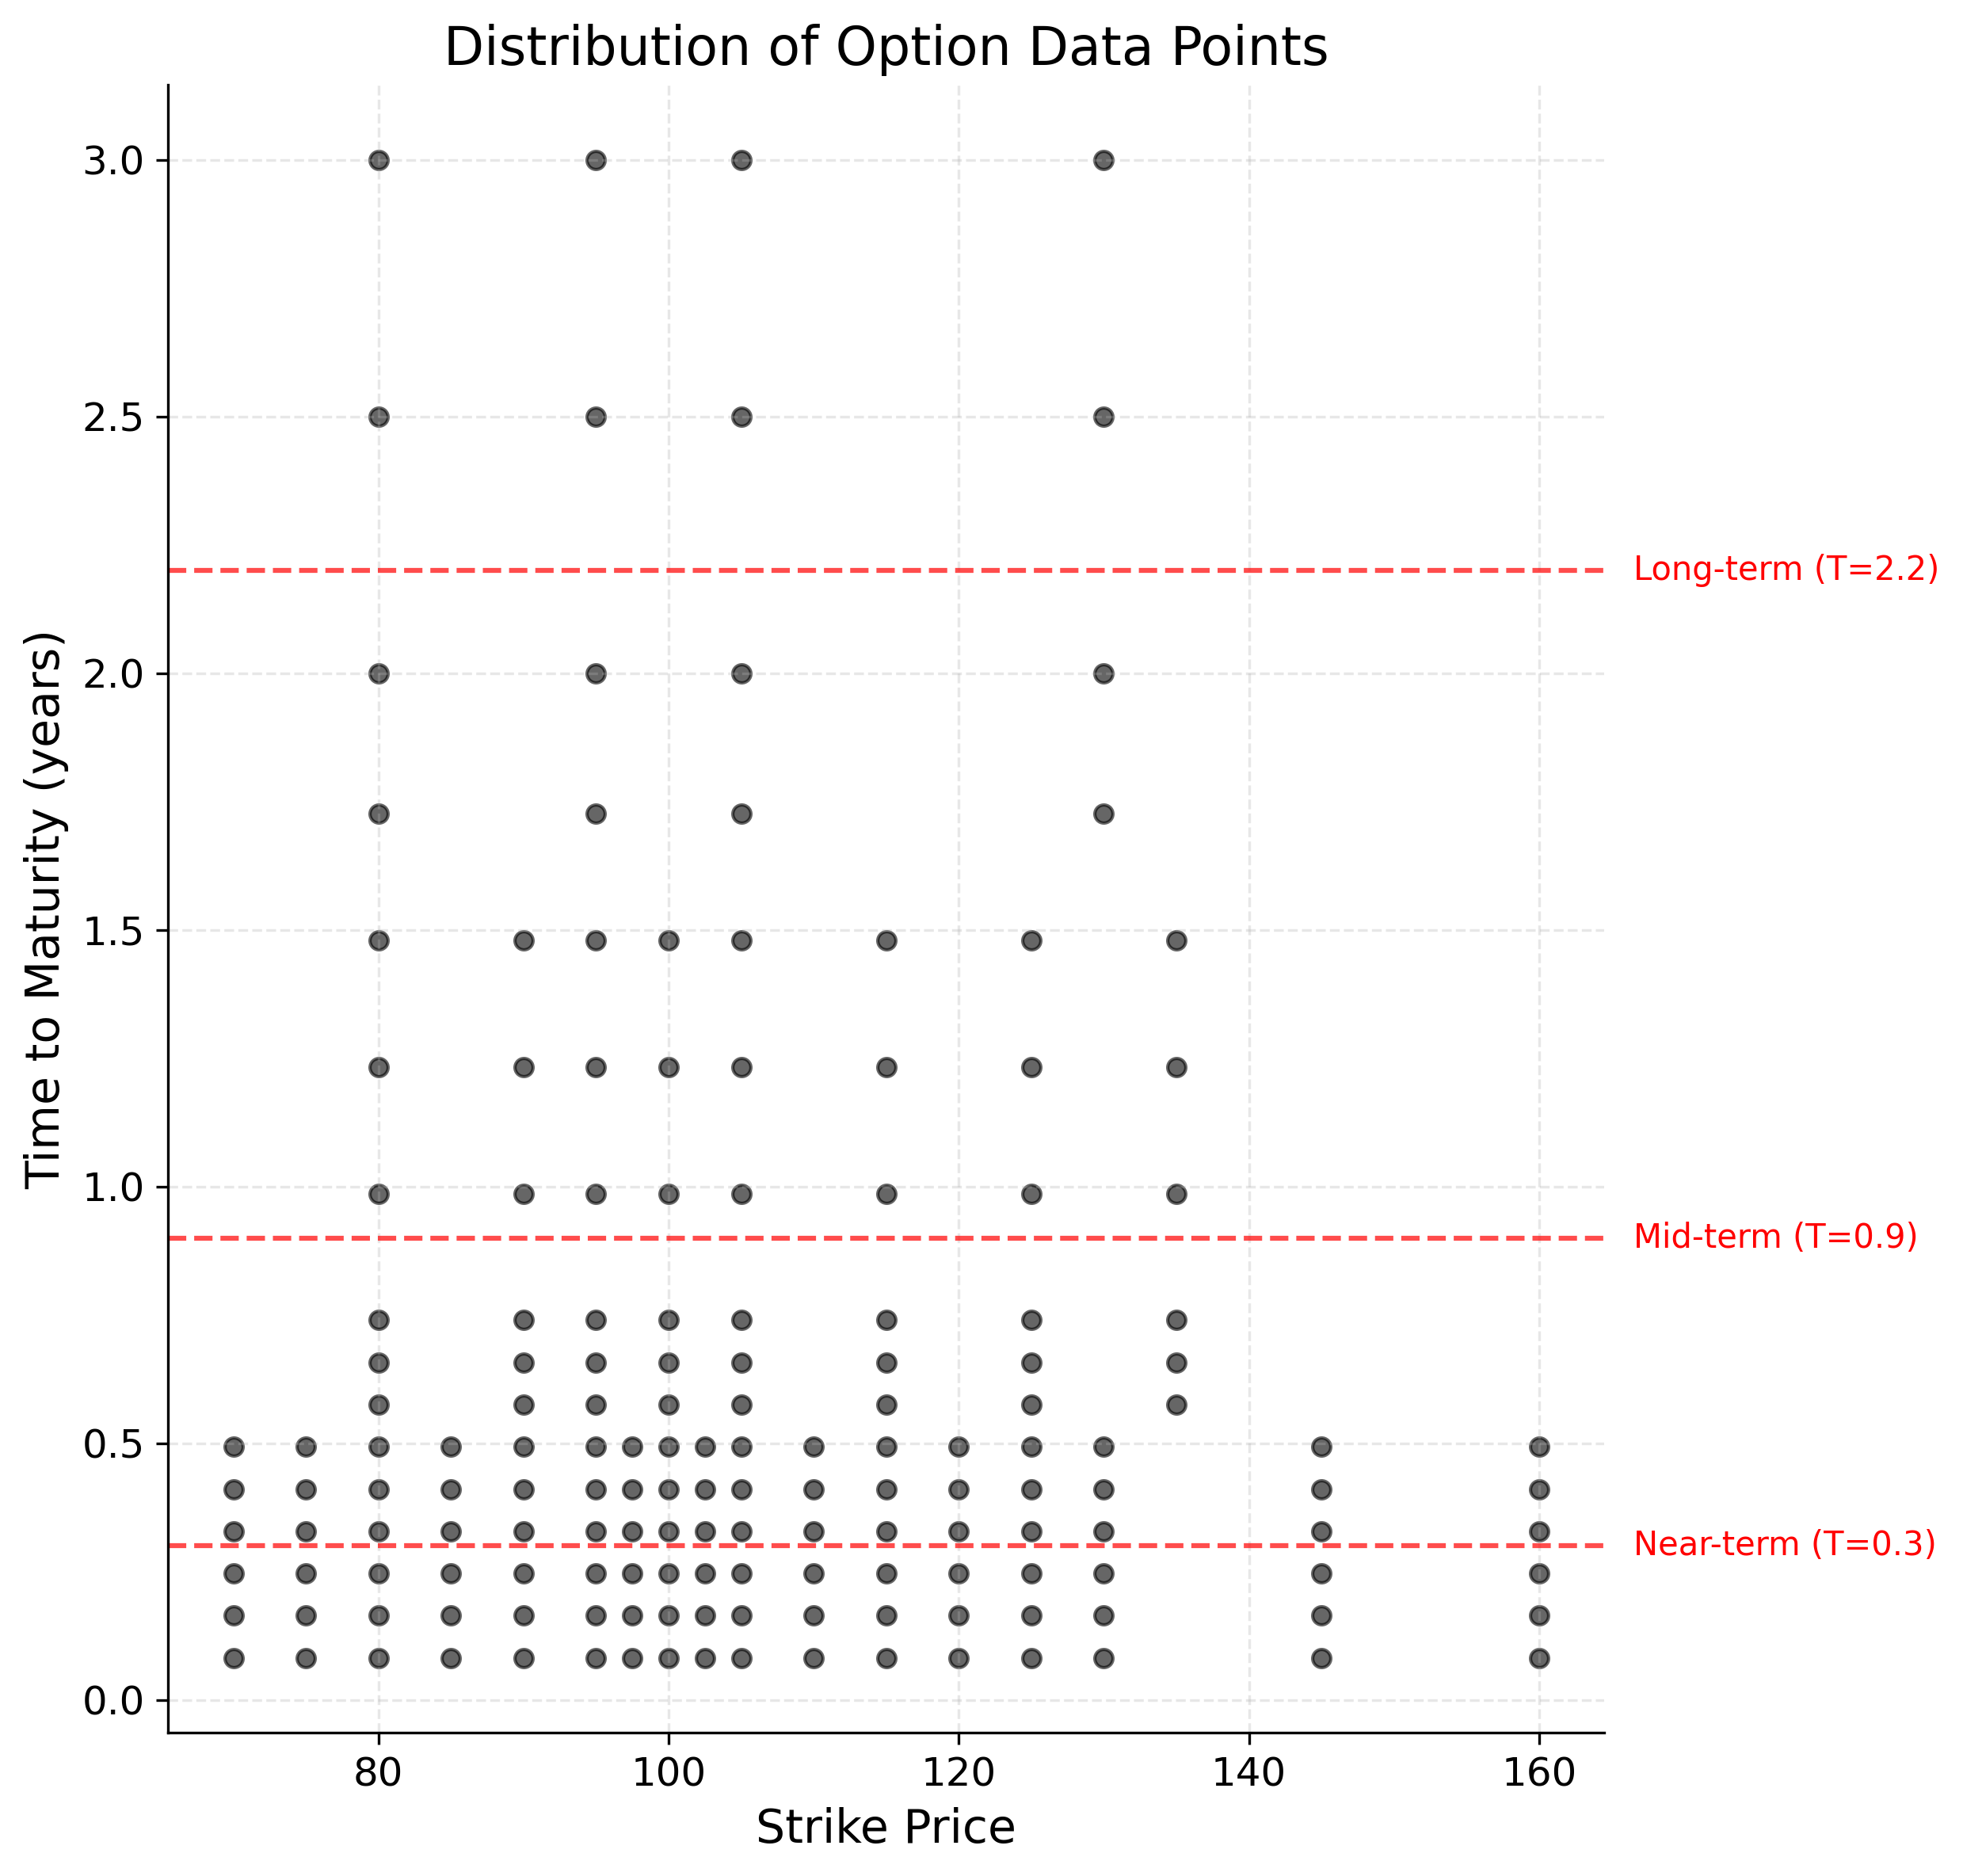
\includegraphics[width=0.5\textwidth]{target_data_distribution.png}
    \caption{Distribution of generated Heston ``market" data points (target task $\mathcal{D}_\mathcal{T}$) in our experiments, by strike price and time to maturity. Dashed red lines indicate evaluation maturities.}
    \label{fig:data_distribution}
\end{figure}

For each contract, we computed the Heston price via Carr-Madan fast Fourier transform method \citep{carr1999option}. Then, we obtained the Black-Scholes implied volatility $\sigma_{\text{mkt}}(K, \tau)$ by inverting the Heston price using a root-finding algorithm. This produced the ``market" dataset $\mathcal{D}_\mathcal{T} = \{(\mathbf{X}_\mathcal{T}, \mathbf{y}_\mathcal{T})\}$, the target task data.

\subsubsection{SABR-Derived Synthetic Data}
The SABR-MTGP used a denser synthetic dataset derived by fitting the SABR model to the Heston data. This involved several steps. First, for each unique maturity $\tau_{(p)} \in \mathbb{T}_{\text{mkt}}$, SABR parameters ($\alpha_{(p)}, \rho_{(p)}, \nu_{(p)}$) were calibrated by minimizing MSE between SABR volatilities $\sigma_{\text{SABR}}$ and market volatilities $\sigma_{\text{mkt}}$ from $\mathcal{D}_{\mathcal{T}}$ ($\beta=0.5$ fixed). We used Nelder-Mead optimization with constraints, yielding calibrated parameters $\{(\alpha_{(p)}, \rho_{(p)}, \nu_{(p)})\}$ for the set $\mathbb{T}_{\text{mkt}}$.

Second, we obtained SABR parameters for any time-to-maturity $\tilde{\tau}$ via piecewise linear interpolation (Equation~\ref{eq:interpolation}) between parameters at the nearest surrounding calibrated maturities in $\mathbb{T}_{\text{mkt}}$. Constant extrapolation was used outside this range. Figure~\ref{fig:sabr_params} shows the calibrated SABR parameters across maturities for the \textit{Base} Heston scenario. The parameters showed term structures consistent with market behavior, supporting the interpolation.
\begin{figure}[htbp]
    \centering
    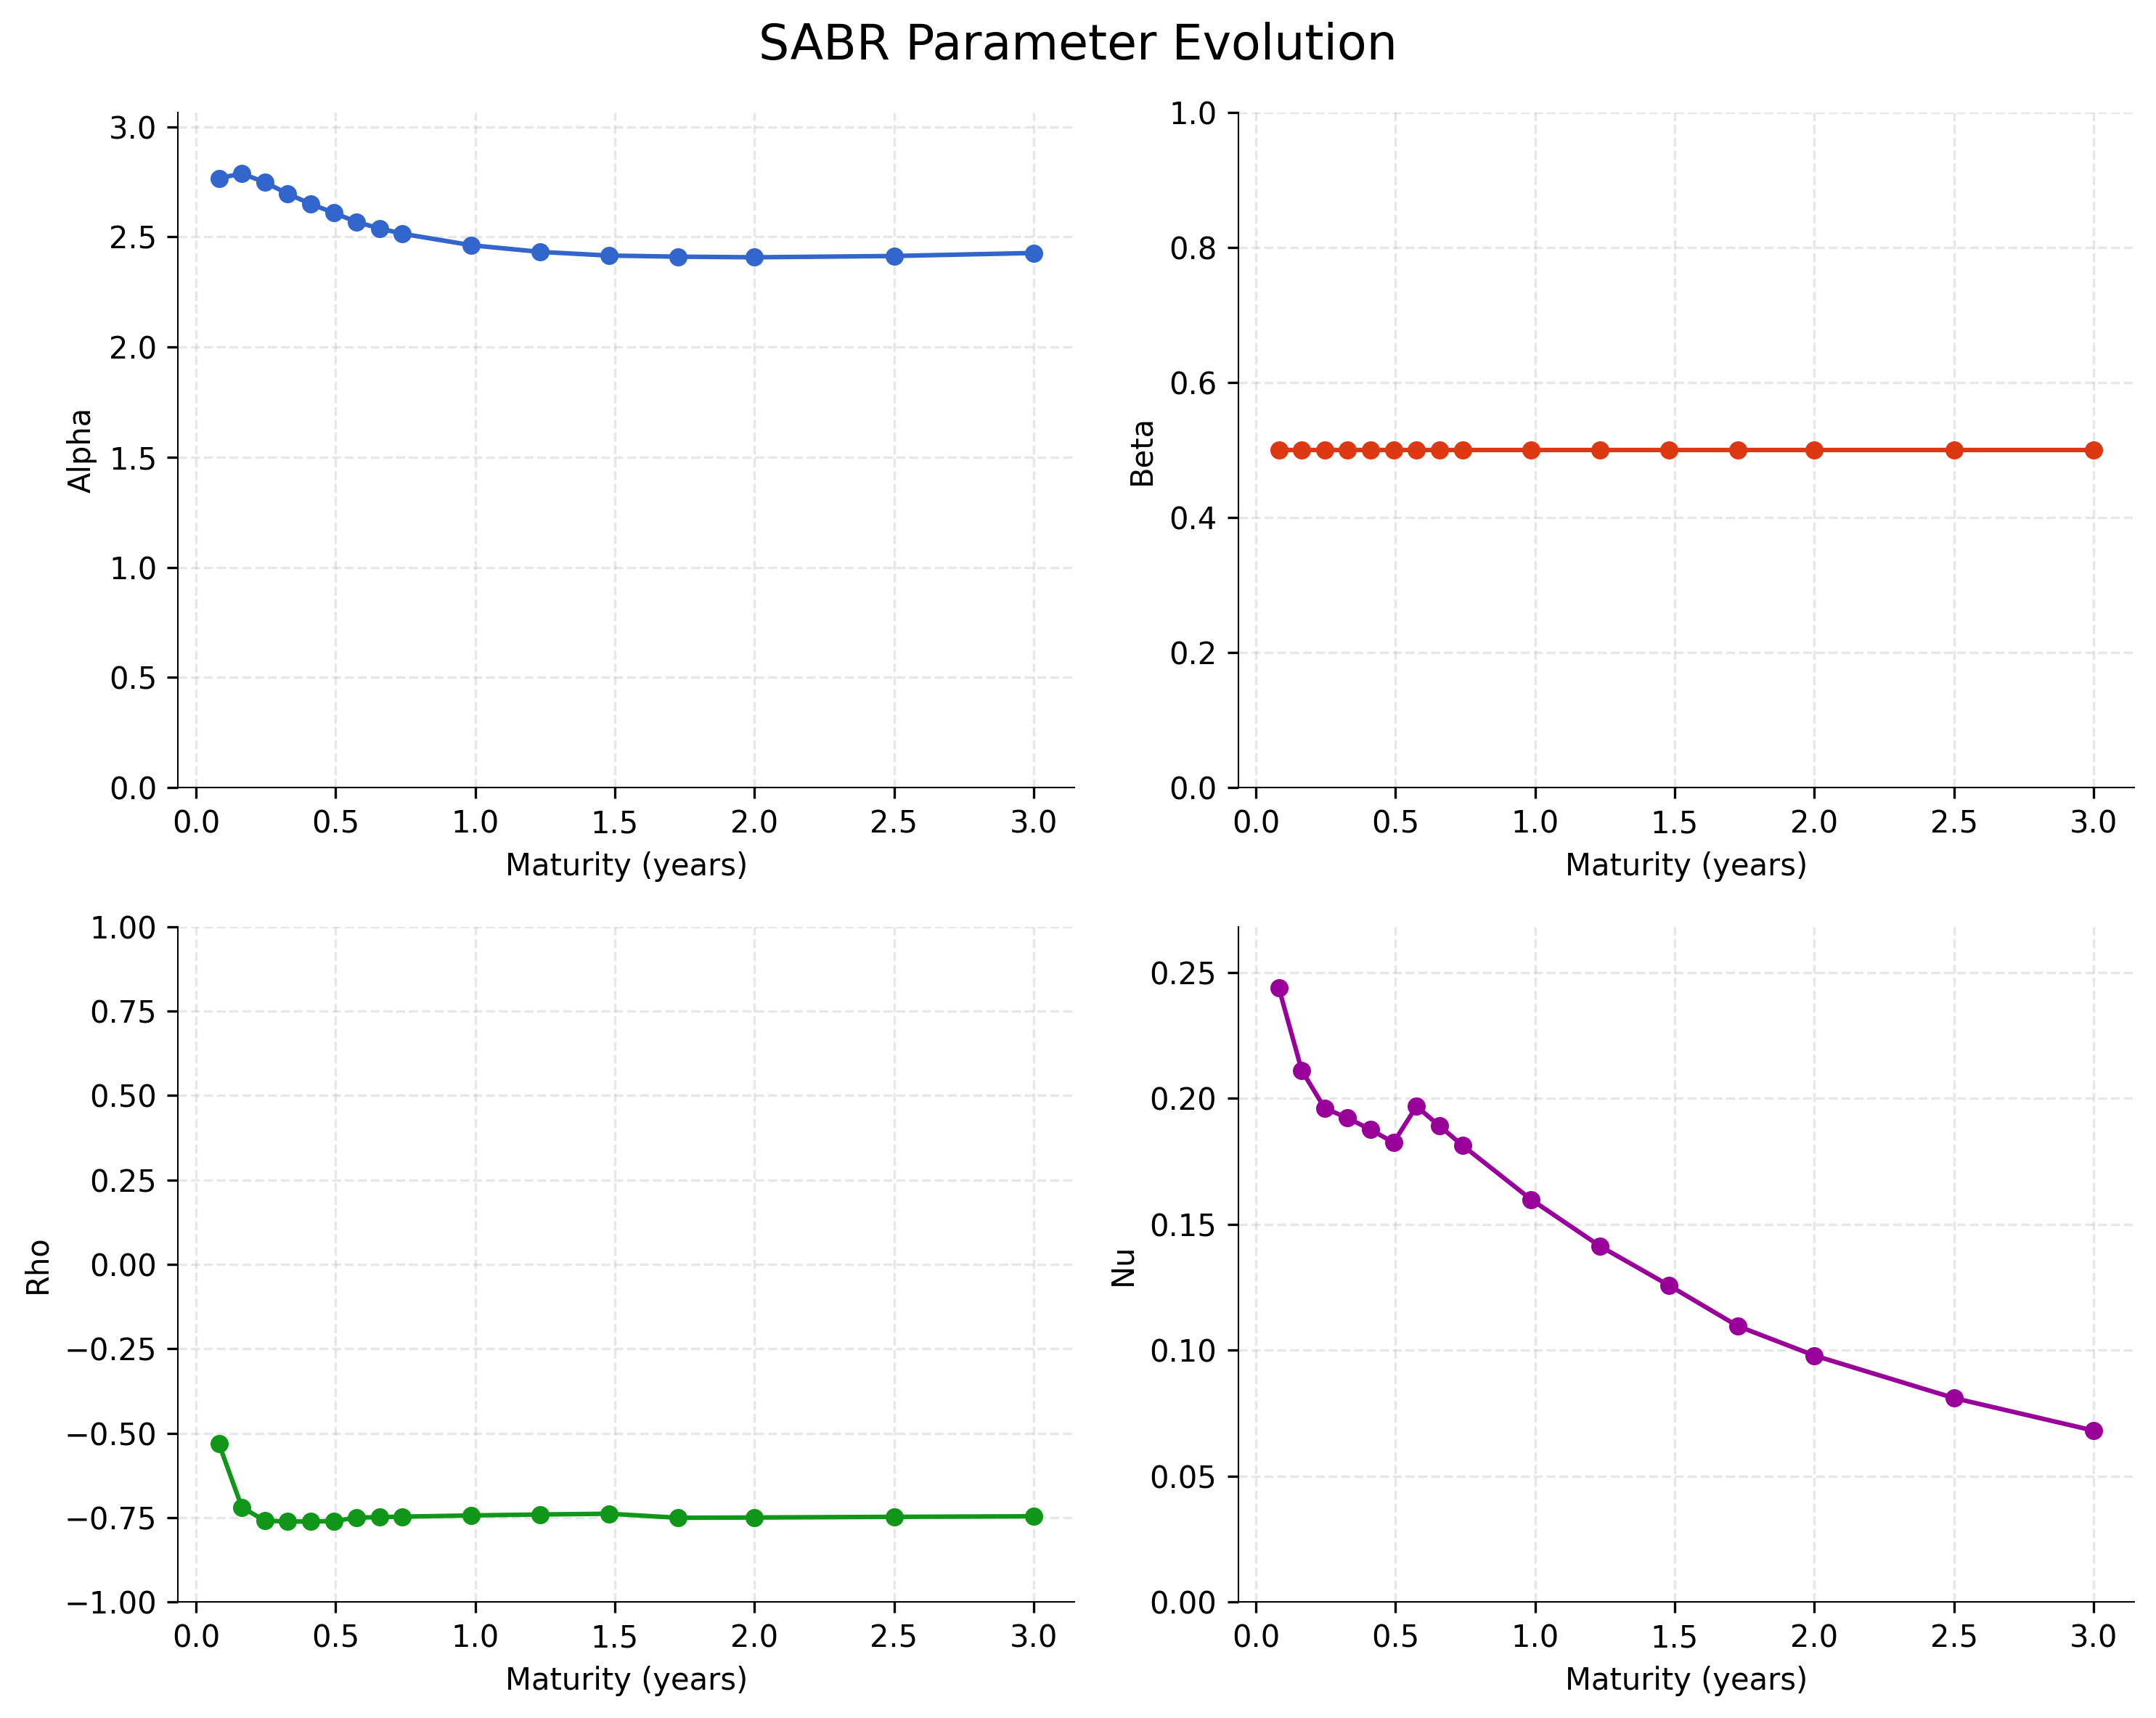
\includegraphics[width=0.5\textwidth]{sabr_parameter_evolution.png}
    \caption{Evolution of calibrated SABR parameters ($\alpha, \beta, \rho, \nu$) across maturity slices for the \textit{Base} Heston scenario. Note $\beta$ was fixed at 0.5 during calibration.}
    \label{fig:sabr_params}
\end{figure}

Third, we defined a dense $35\times35$ grid $(\tilde{K}_j, \tilde{\tau}_j)$, covering strike range ($K \in [70, 160]$) and maturity range ( $\tau \in [0.08, 3.0]$). At each grid point, we used the interpolated/extrapolated SABR parameters with the Hagan formula (Equation~\ref{eq:sabr_detailed}) to compute synthetic implied volatility $y_{\mathcal{S},j} = \sigma_{\text{SABR}}(\tilde{K}_j, F_{\tilde{\tau}_j},\tilde{\tau}_j;\alpha_{\tilde{\tau}_j}, \beta, \rho_{{\tilde\tau}_j}, \nu_{{\tilde\tau}_j}).$

Finally, we added small Gaussian noise $\epsilon_{\mathcal{S}} \sim \mathcal{N}(0, 0.01^2)$ to the synthetic data. This generated the synthetic source dataset $\mathcal{D}_\mathcal{S} = \{(\mathbf{X}_\mathcal{S}, \mathbf{y}_\mathcal{S})\}$.

\subsection{Comparative Models and Training}

We compared three approaches for constructing the IVS. First, \textbf{SABR Interpolation}, a parametric baseline using calibrated and interpolated SABR parameters with the Hagan formula (Equation~\ref{eq:sabr_detailed}). Second, a \textbf{Single-Task Gaussian Process (GP)} trained only on the sparse Heston ``market" data $\mathcal{D}_\mathcal{T}$. This GP used a Matérn 5/2 kernel on $(K, \tau)$ inputs and learned hyperparameters via L-BFGS optimization of marginal likelihood. Third, the proposed \textbf{SABR-Informed Multi-Task GP (SABR-MTGP)}, our transfer learning framework. It was trained jointly on synthetic source data $\mathcal{D}_\mathcal{S}$ and market target data $\mathcal{D}_\mathcal{T}$, using the ICM structure with a shared Matérn 5/2 input kernel and a task kernel based on learned one-dimensional embeddings.

\subsection{Evaluation Framework and Robustness Analysis}

We evaluated model performance against the Heston ground truth on a predefined evaluation grid for fair comparison. This grid, separate from training data, included points $(K_\ast, \tau_\ast)$ spanning a relevant moneyness range (e.g., $K_\ast/S_0 \in [0.8, 1.4]$) at specific test maturities $\tau_\ast$ (e.g., 0.3, 0.9, 2.2 years) representing near-, mid-, and long-term. For each evaluation point, we computed the ground truth Heston IV using a high-precision FFT approach with the Heston characteristic function, followed by numerical inversion to obtain corresponding implied volatility. 

Each model (SABR Interpolation, GP, SABR-MTGP) predicted $\hat{\sigma}(K_\ast, \tau_\ast)$ on this grid. We measured performance using Root Mean Squared Error (RMSE) and Mean Absolute Error (MeanAE) against the ground truth $\sigma_{\text{Heston}}(K_\ast, \tau_\ast)$, calculated over valid predictions.

To assess robustness, we repeated experiments using ten Heston parameter configurations (Table~\ref{tab:heston_params}), including the \textit{Base} scenario. These settings simulated various market dynamics by altering parameters like mean reversion $\kappa$, volatility levels $\theta, \nu_{\text{vol}}$, correlation $\rho$, and initial term structure $v_0$ vs $\theta$. This allowed analysis across different market conditions. Robustness evaluation focused on metrics at distinct test maturities. We also analyzed the MTGP's learned task correlation and variance decomposition for each scenario to understand its adaptive information-sharing.

\begin{table}[htbp]
    \centering
    \caption{Heston Parameter Configurations for Robustness Analysis. Common parameters are $S_0=100, r=0.03, q=0.01$.}
    \label{tab:heston_params}
    \begin{tabular}{@{}lccccc@{}}
        \toprule
        Setting Name & $\kappa$ & $\theta$ & $\nu_{\text{vol}}$ & $\rho$ & $v_0$ \\
        \midrule
        Base                 & 1.0 & 0.09 & 0.8 & -0.8 & 0.09 \\
        Moderate Mean-Rev    & 2.0 & 0.09 & 0.8 & -0.8 & 0.09 \\
        Low Mean-Rev         & 0.5 & 0.09 & 0.8 & -0.8 & 0.09 \\
        High Vol-Regime      & 1.0 & 0.16 & 0.9 & -0.8 & 0.16 \\
        Low Vol-Regime       & 1.0 & 0.04 & 0.4 & -0.8 & 0.04 \\
        Moderate Correlation & 1.0 & 0.09 & 0.8 & -0.5 & 0.09 \\
        Strong Correlation   & 1.0 & 0.09 & 0.8 & -0.9 & 0.09 \\
        Term Structure Up    & 1.0 & 0.16 & 0.8 & -0.8 & 0.09 \\
        Term Structure Down  & 1.0 & 0.04 & 0.8 & -0.8 & 0.16 \\
        Mixed Regime         & 1.5 & 0.12 & 0.6 & -0.6 & 0.12 \\
        \bottomrule
    \end{tabular}
\end{table}

\section{Results and Discussion} \label{sec:results}

This section presents our findings on SABR-MTGP performance compared with SABR interpolation and the standard GP. We first analyze performance under the \textit{Base} Heston scenario, then examine robustness across various market conditions.

\subsection{Performance in the Base Scenario}

Figures~\ref{fig:iv_near}, \ref{fig:iv_mid}, and \ref{fig:iv_long} show fitted implied volatility curves from the three models compared against Heston ground truth, for near-term ($\tau=0.30$), mid-term ($\tau=0.90$), and long-term ($\tau=2.20$) maturities in the \textit{Base} scenario. Each figure includes fitted curves and residuals.

\begin{figure}[htbp]
    \centering
    \begin{subfigure}[b]{0.48\textwidth}
        \centering
        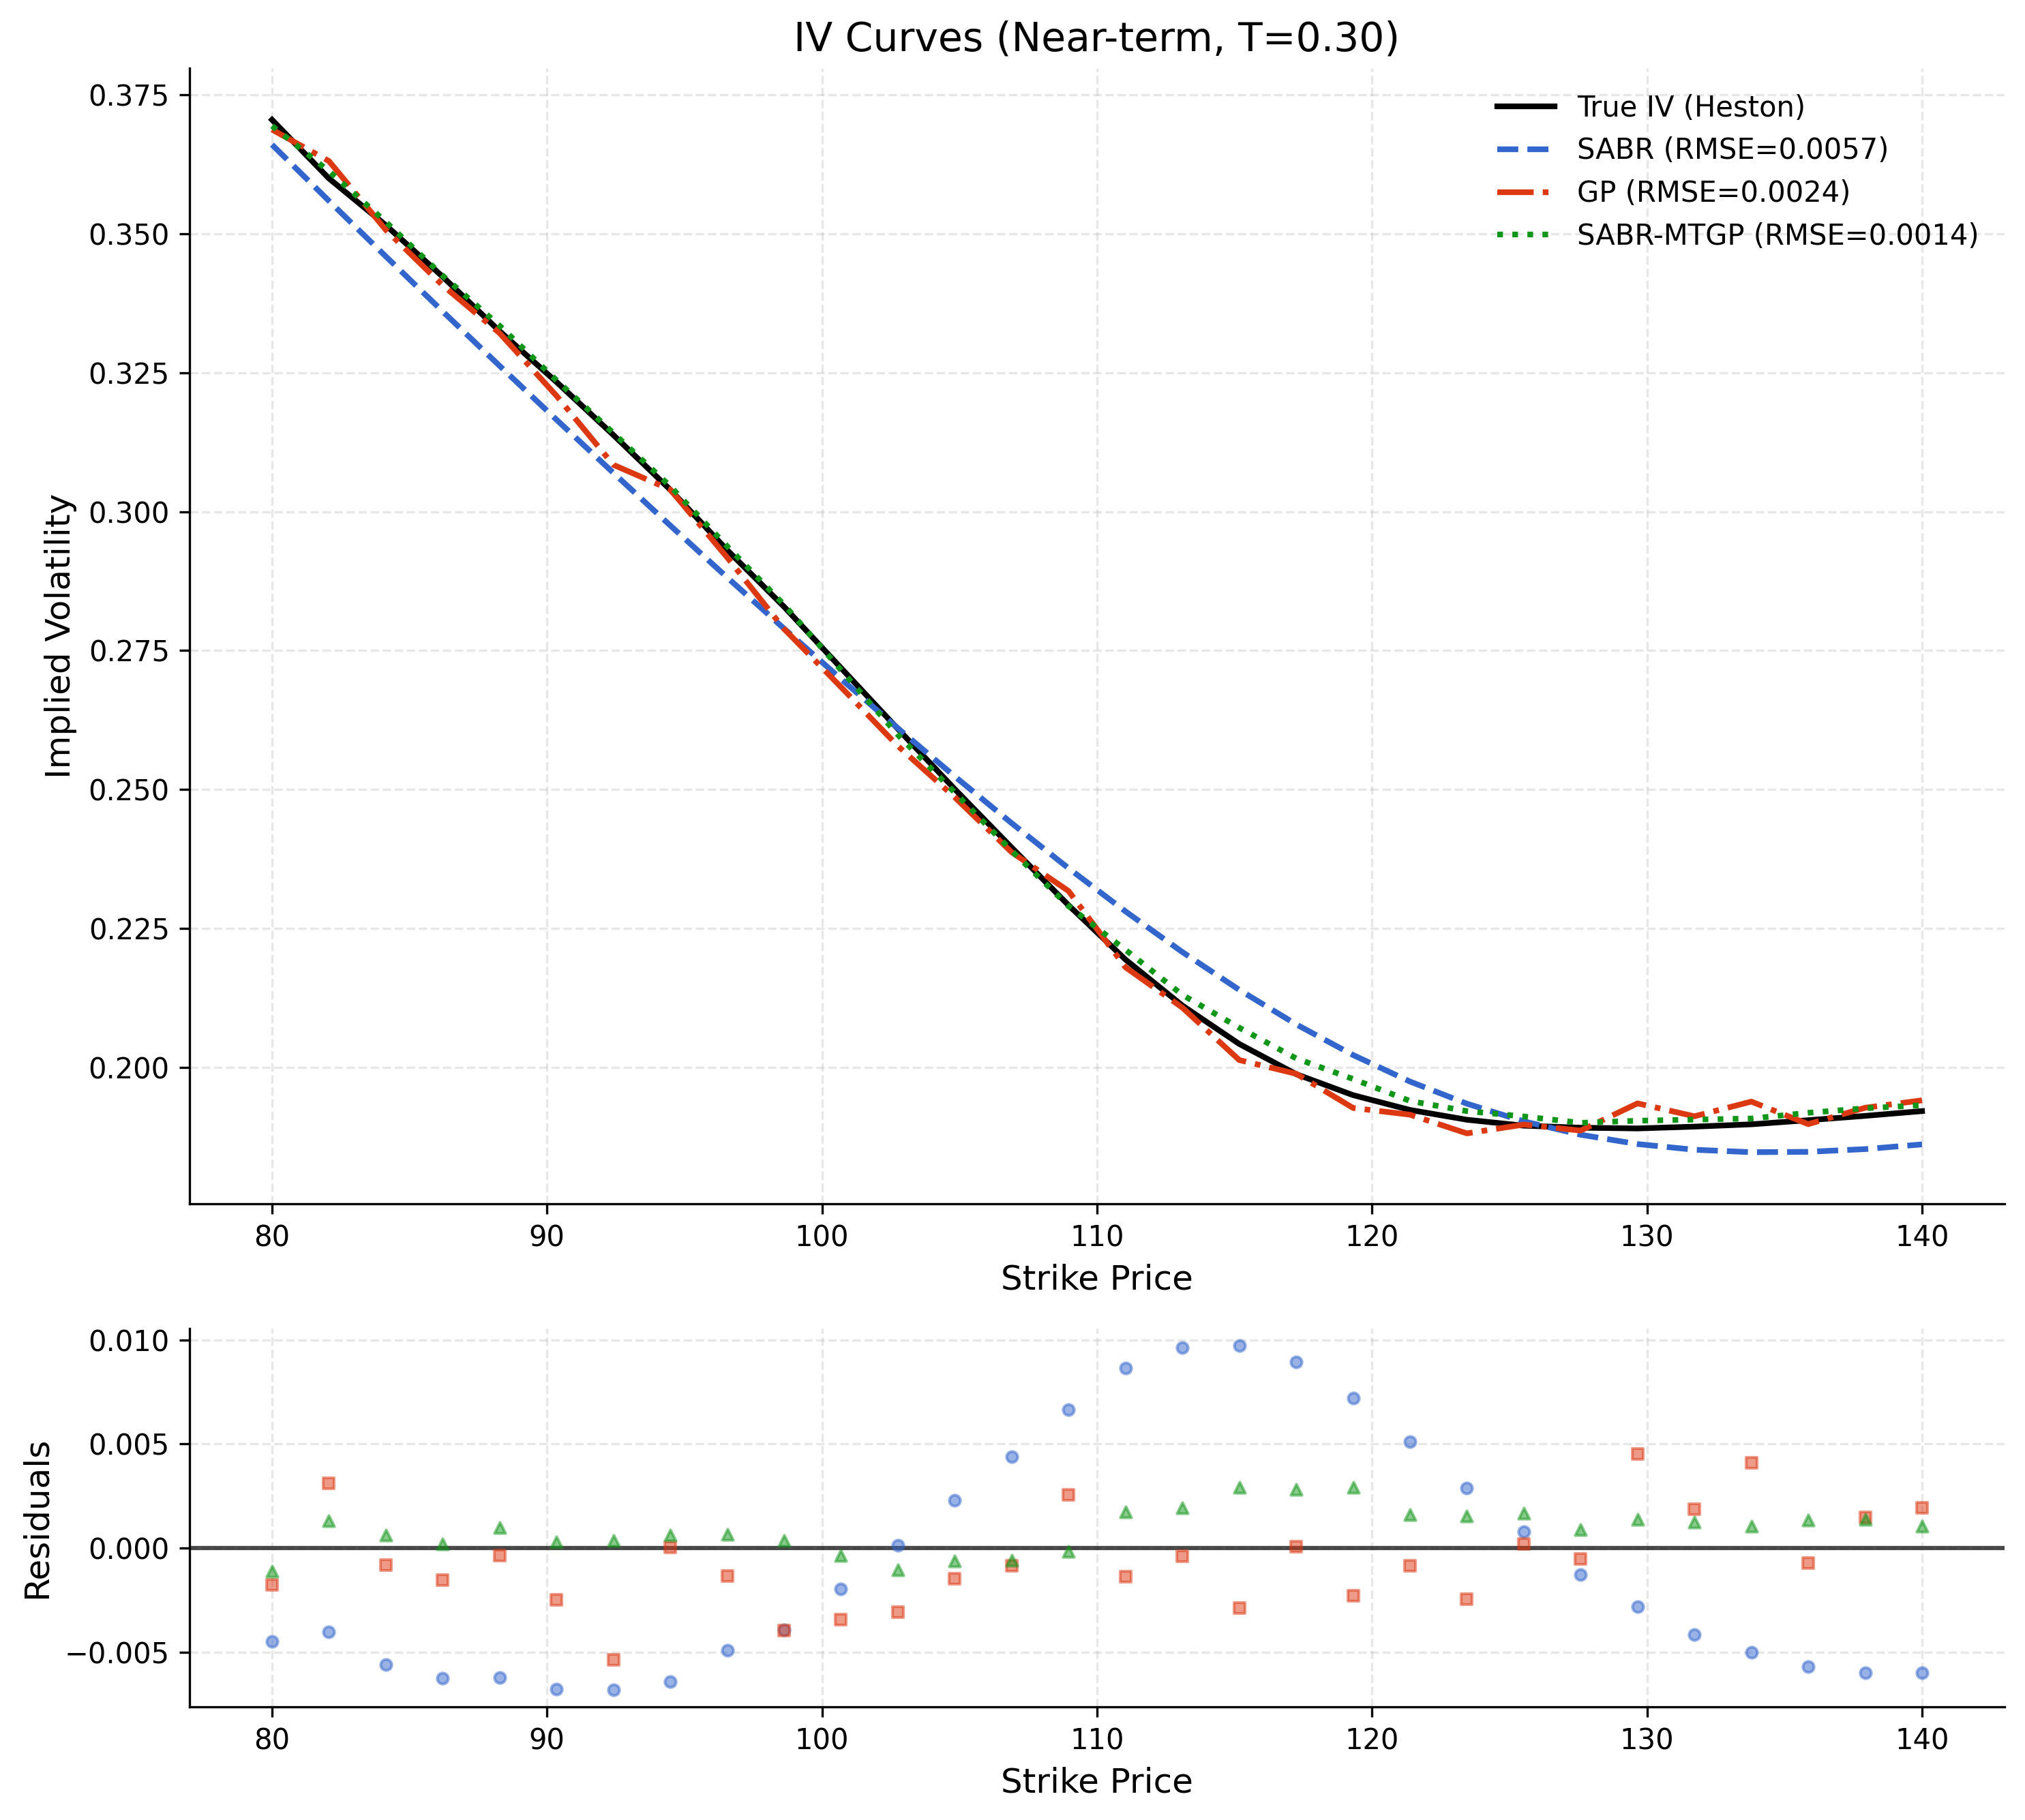
\includegraphics[width=\textwidth]{iv_curves_Base_Near-term.png}
        \caption{Near-term ($\tau=0.30$).}
        \label{fig:iv_near}
    \end{subfigure}
    \hfill % Optional: adds space between subfigures
    \begin{subfigure}[b]{0.48\textwidth}
        \centering
        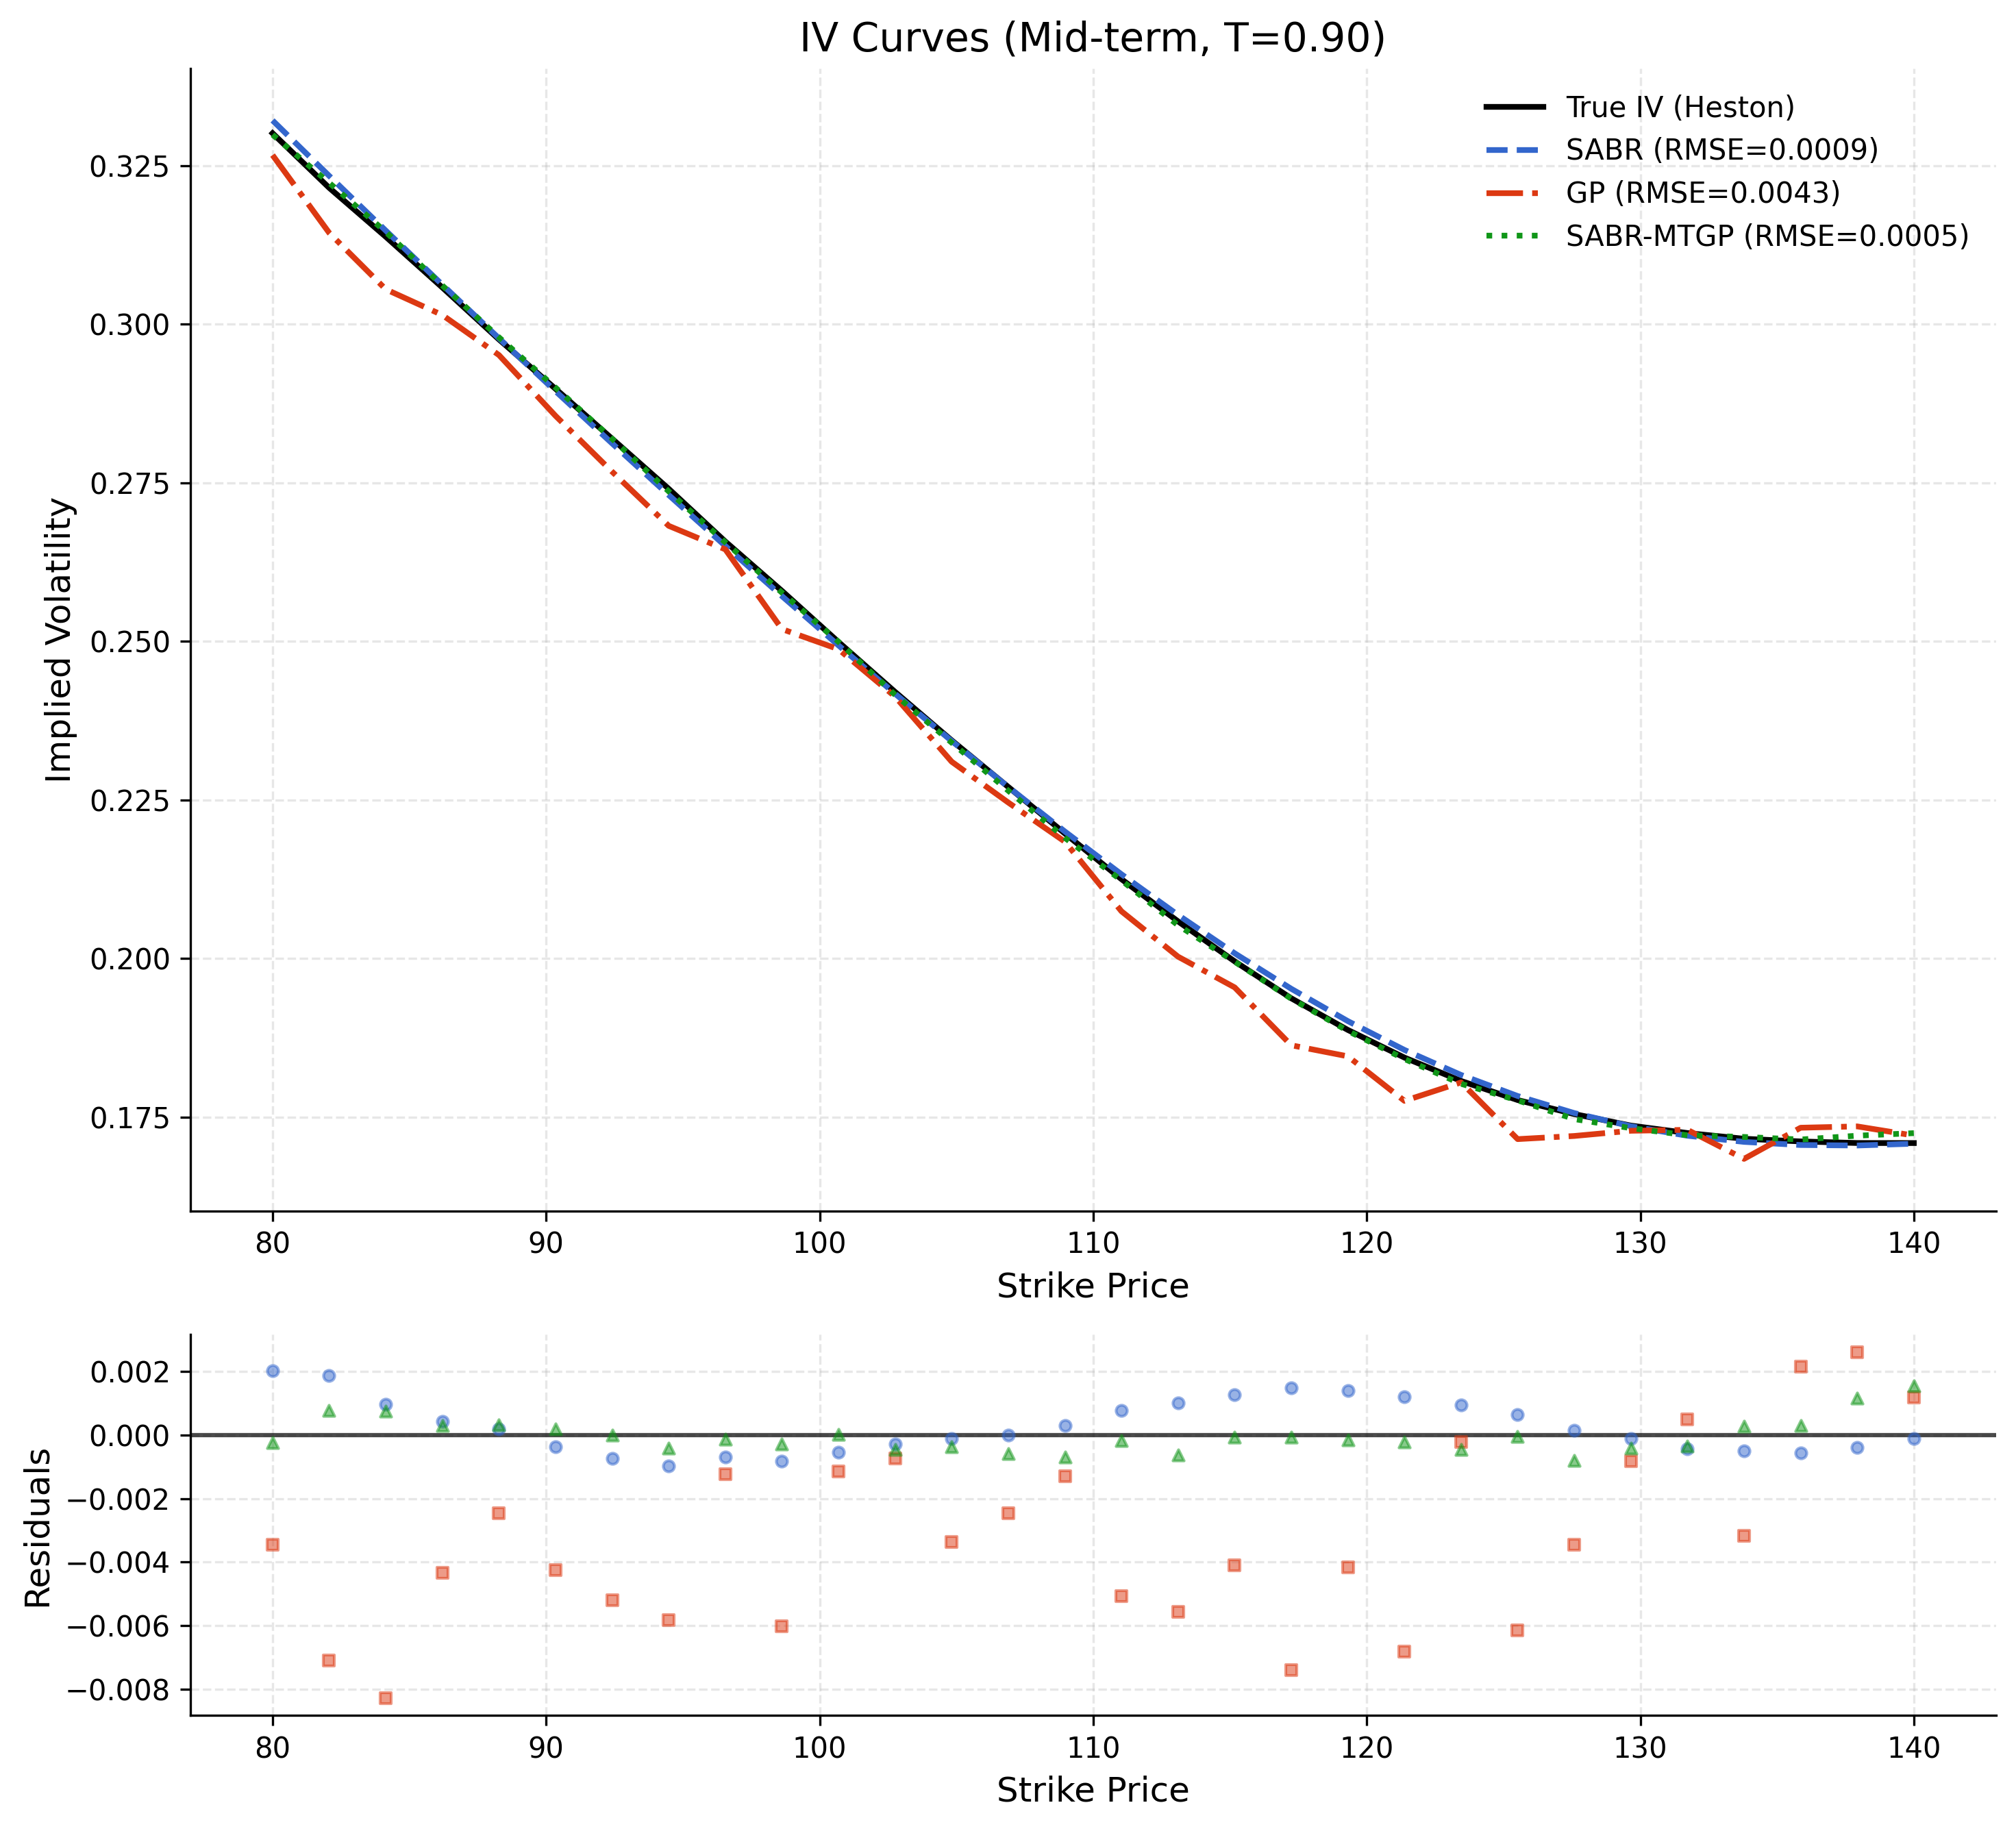
\includegraphics[width=\textwidth]{iv_curves_Base_Mid-term.png}
        \caption{Mid-term ($\tau=0.90$).}
        \label{fig:iv_mid}
    \end{subfigure}

    \vspace{1em} % Add some vertical space before the next row

    \begin{subfigure}[b]{0.48\textwidth} % Adjust width as needed, centering handled by figure environment
        \centering
        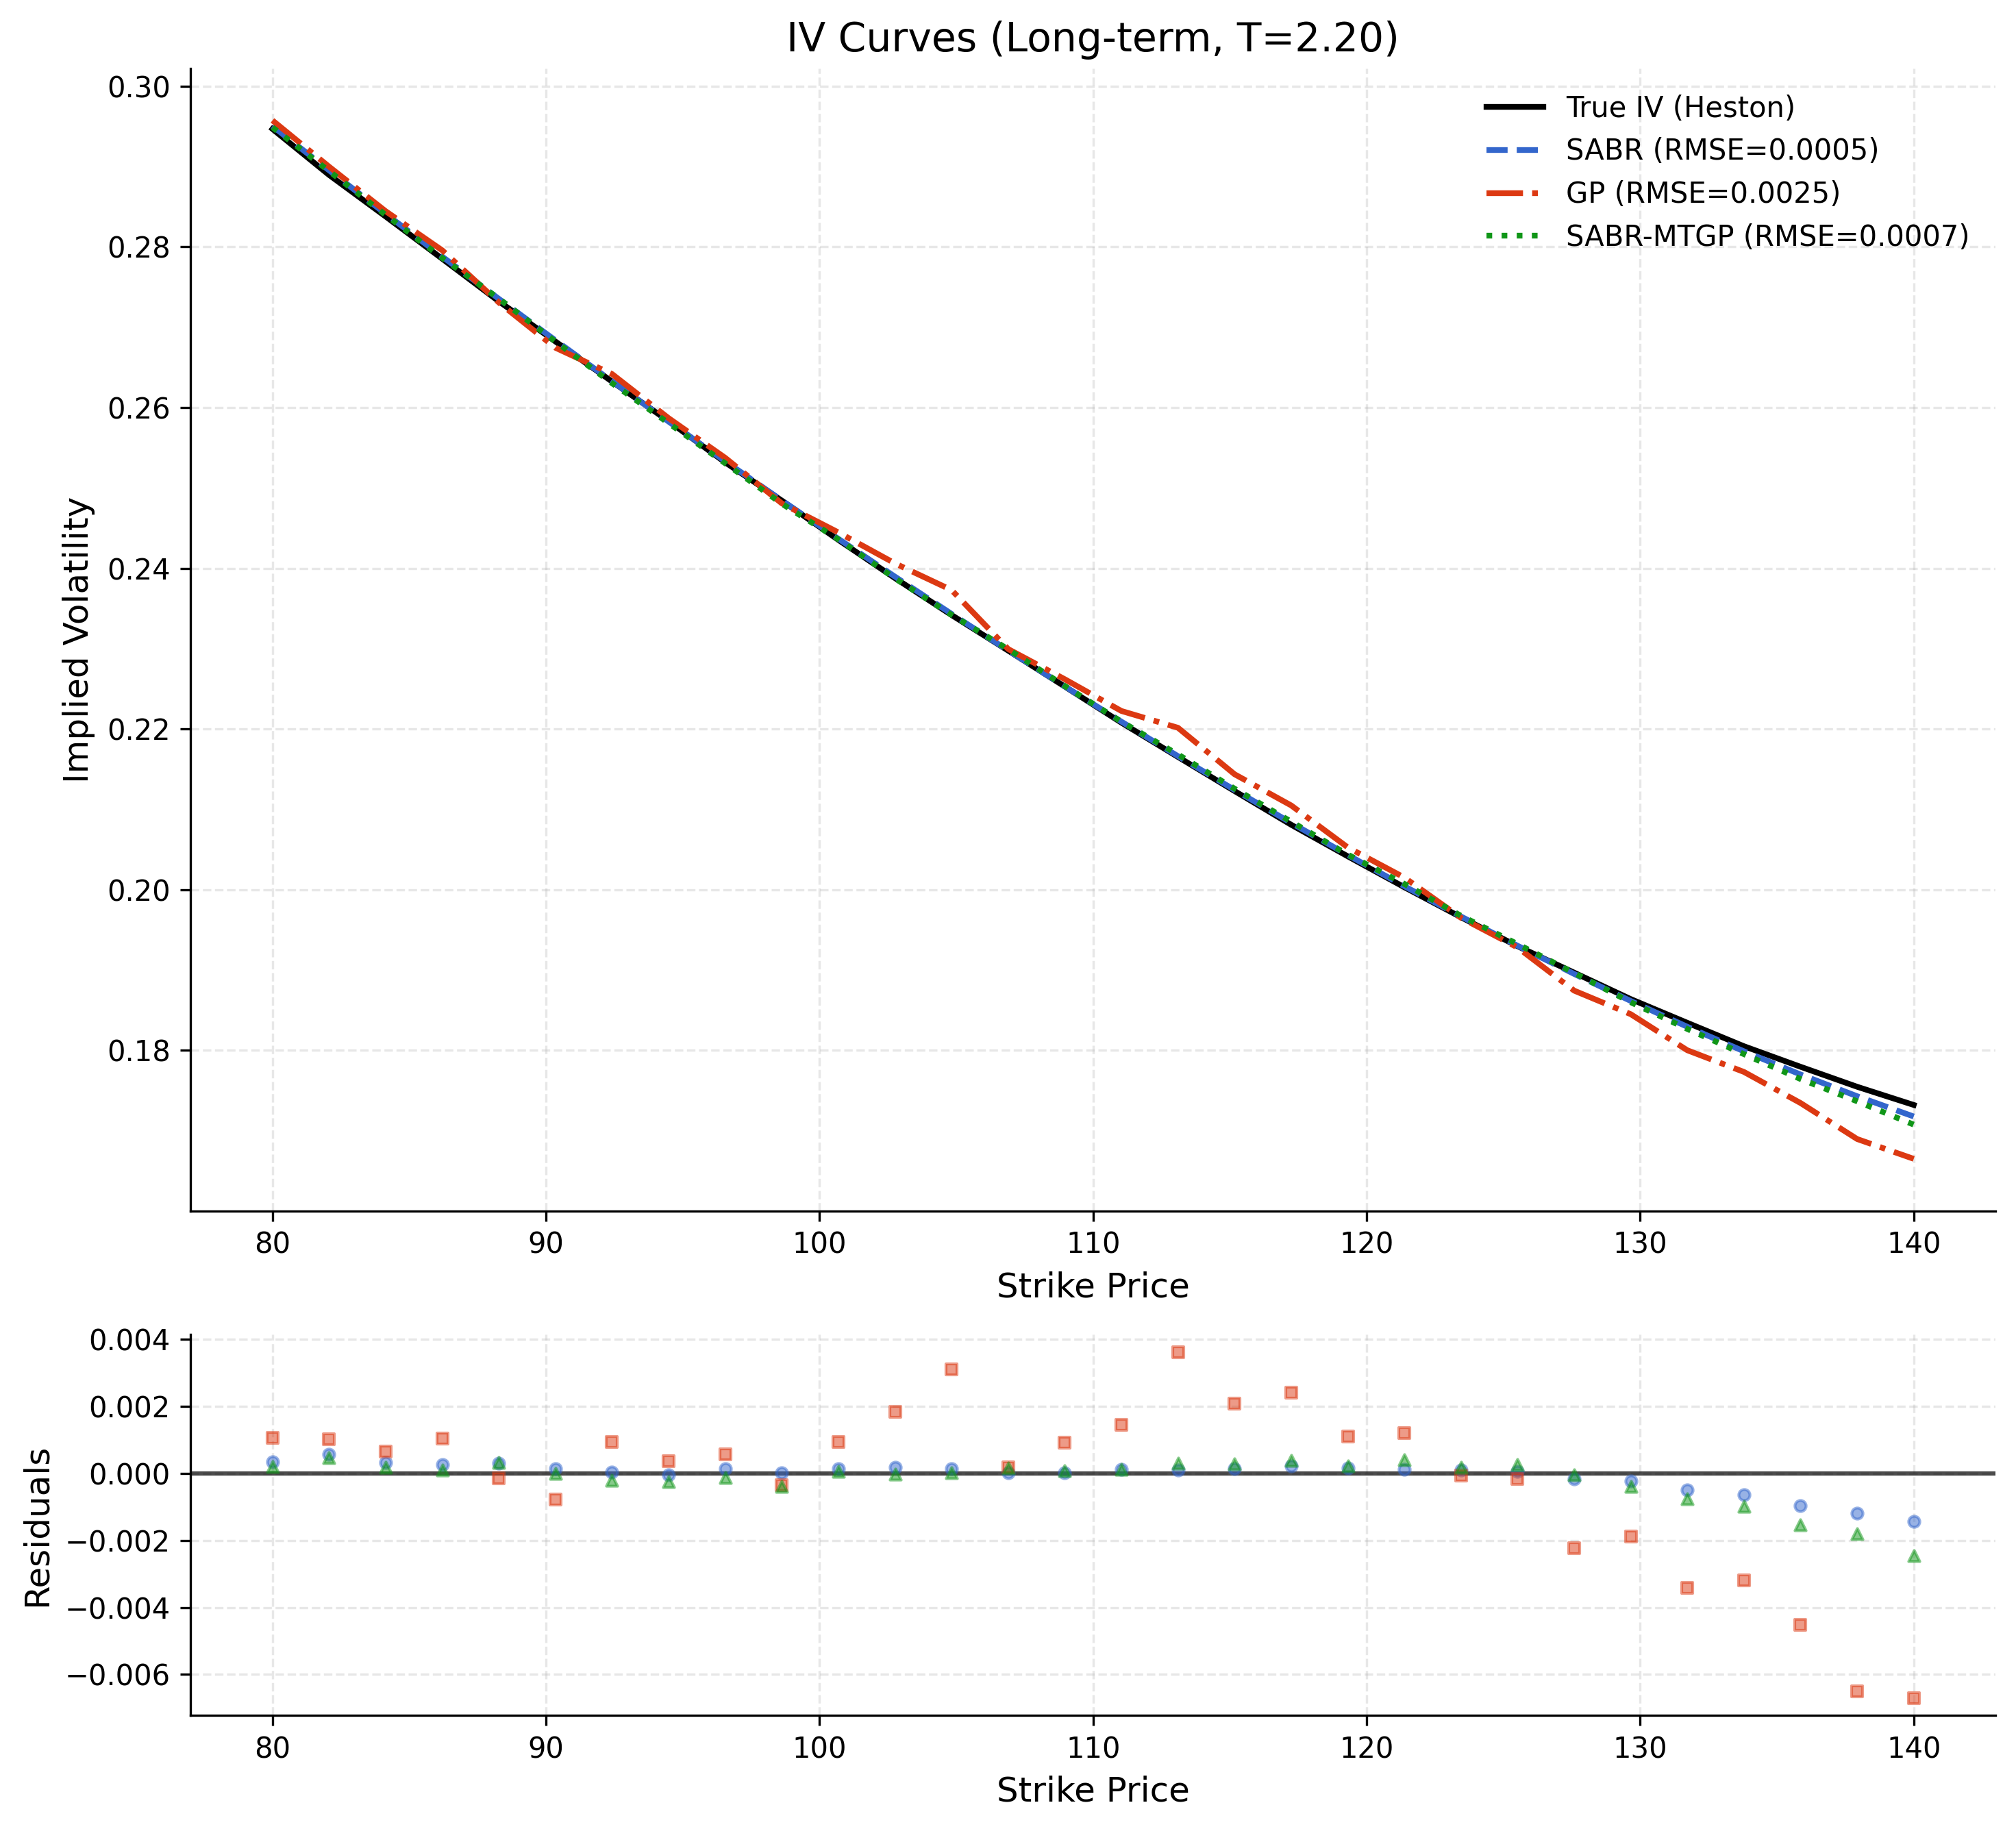
\includegraphics[width=\textwidth]{iv_curves_Base_Long-term.png}
        \caption{Long-term ($\tau=2.20$).}
        \label{fig:iv_long}
    \end{subfigure}
    \caption{Implied volatility curve comparison and residuals under the \textit{Base} Heston scenario for (a) Near-term, (b) Mid-term, and (c) Long-term maturities.}
    \label{fig:base_scenario_curves}
\end{figure}

The results showed different performance patterns across the term structure. For near-term maturity (Figure~\ref{fig:iv_near}), where market data is relatively dense, SABR-MTGP achieved the most accurate fit across strikes (RMSE=0.0014). The standard GP (RMSE=0.0024) showed systematic deviations, suggesting difficulty capturing the precise smile pattern. Direct SABR interpolation (RMSE=0.0057) struggled with curvature, showing systematic errors consistent with limitations of its parametric form in matching these Heston dynamics.

Moving to mid-term maturity (Figure~\ref{fig:iv_mid}), data sparsity increased. SABR-MTGP continued to provide the closest fit (RMSE=0.0005). SABR interpolation also performed very well (RMSE=0.0009), capturing the overall shape effectively. However, the standard GP (RMSE=0.0043) showed larger and more scattered errors, particularly for strikes away from the money. 

For long-term maturity (Figure~\ref{fig:iv_long}), SABR interpolation performed best according to RMSE (0.0005), benefiting from its structure to provide a reasonable approximation. SABR-MTGP also achieved very good accuracy (RMSE=0.0007). The standard GP (RMSE=0.0025) exhibited notably higher errors compared to the other two methods, with residuals spanning approximately from $-0.006$ to $+0.002$ volatility points, indicating difficulties in generalizing from the sparse long-term data.

These findings highlight the advantages of our hybrid approach. In data-rich regions (near-term), SABR-MTGP combined market data with structural guidance to outperform alternatives. As data gets sparser (mid- to long-term), it used SABR structure effectively while retaining flexibility to adapt to Heston dynamics, balancing SABR's rigidity and standard GP's data dependence.

\subsection{Robustness Across Market Conditions}

The performance heatmaps in Figures~\ref{fig:heatmap_near}, \ref{fig:heatmap_mid}, and \ref{fig:heatmap_long} summarized model accuracy (RMSE and MeanAE) across the ten Heston parameter settings, evaluated at near-, mid-, and long-term horizons. Lighter shades indicated lower errors.

\begin{figure}[htbp]
    \centering
    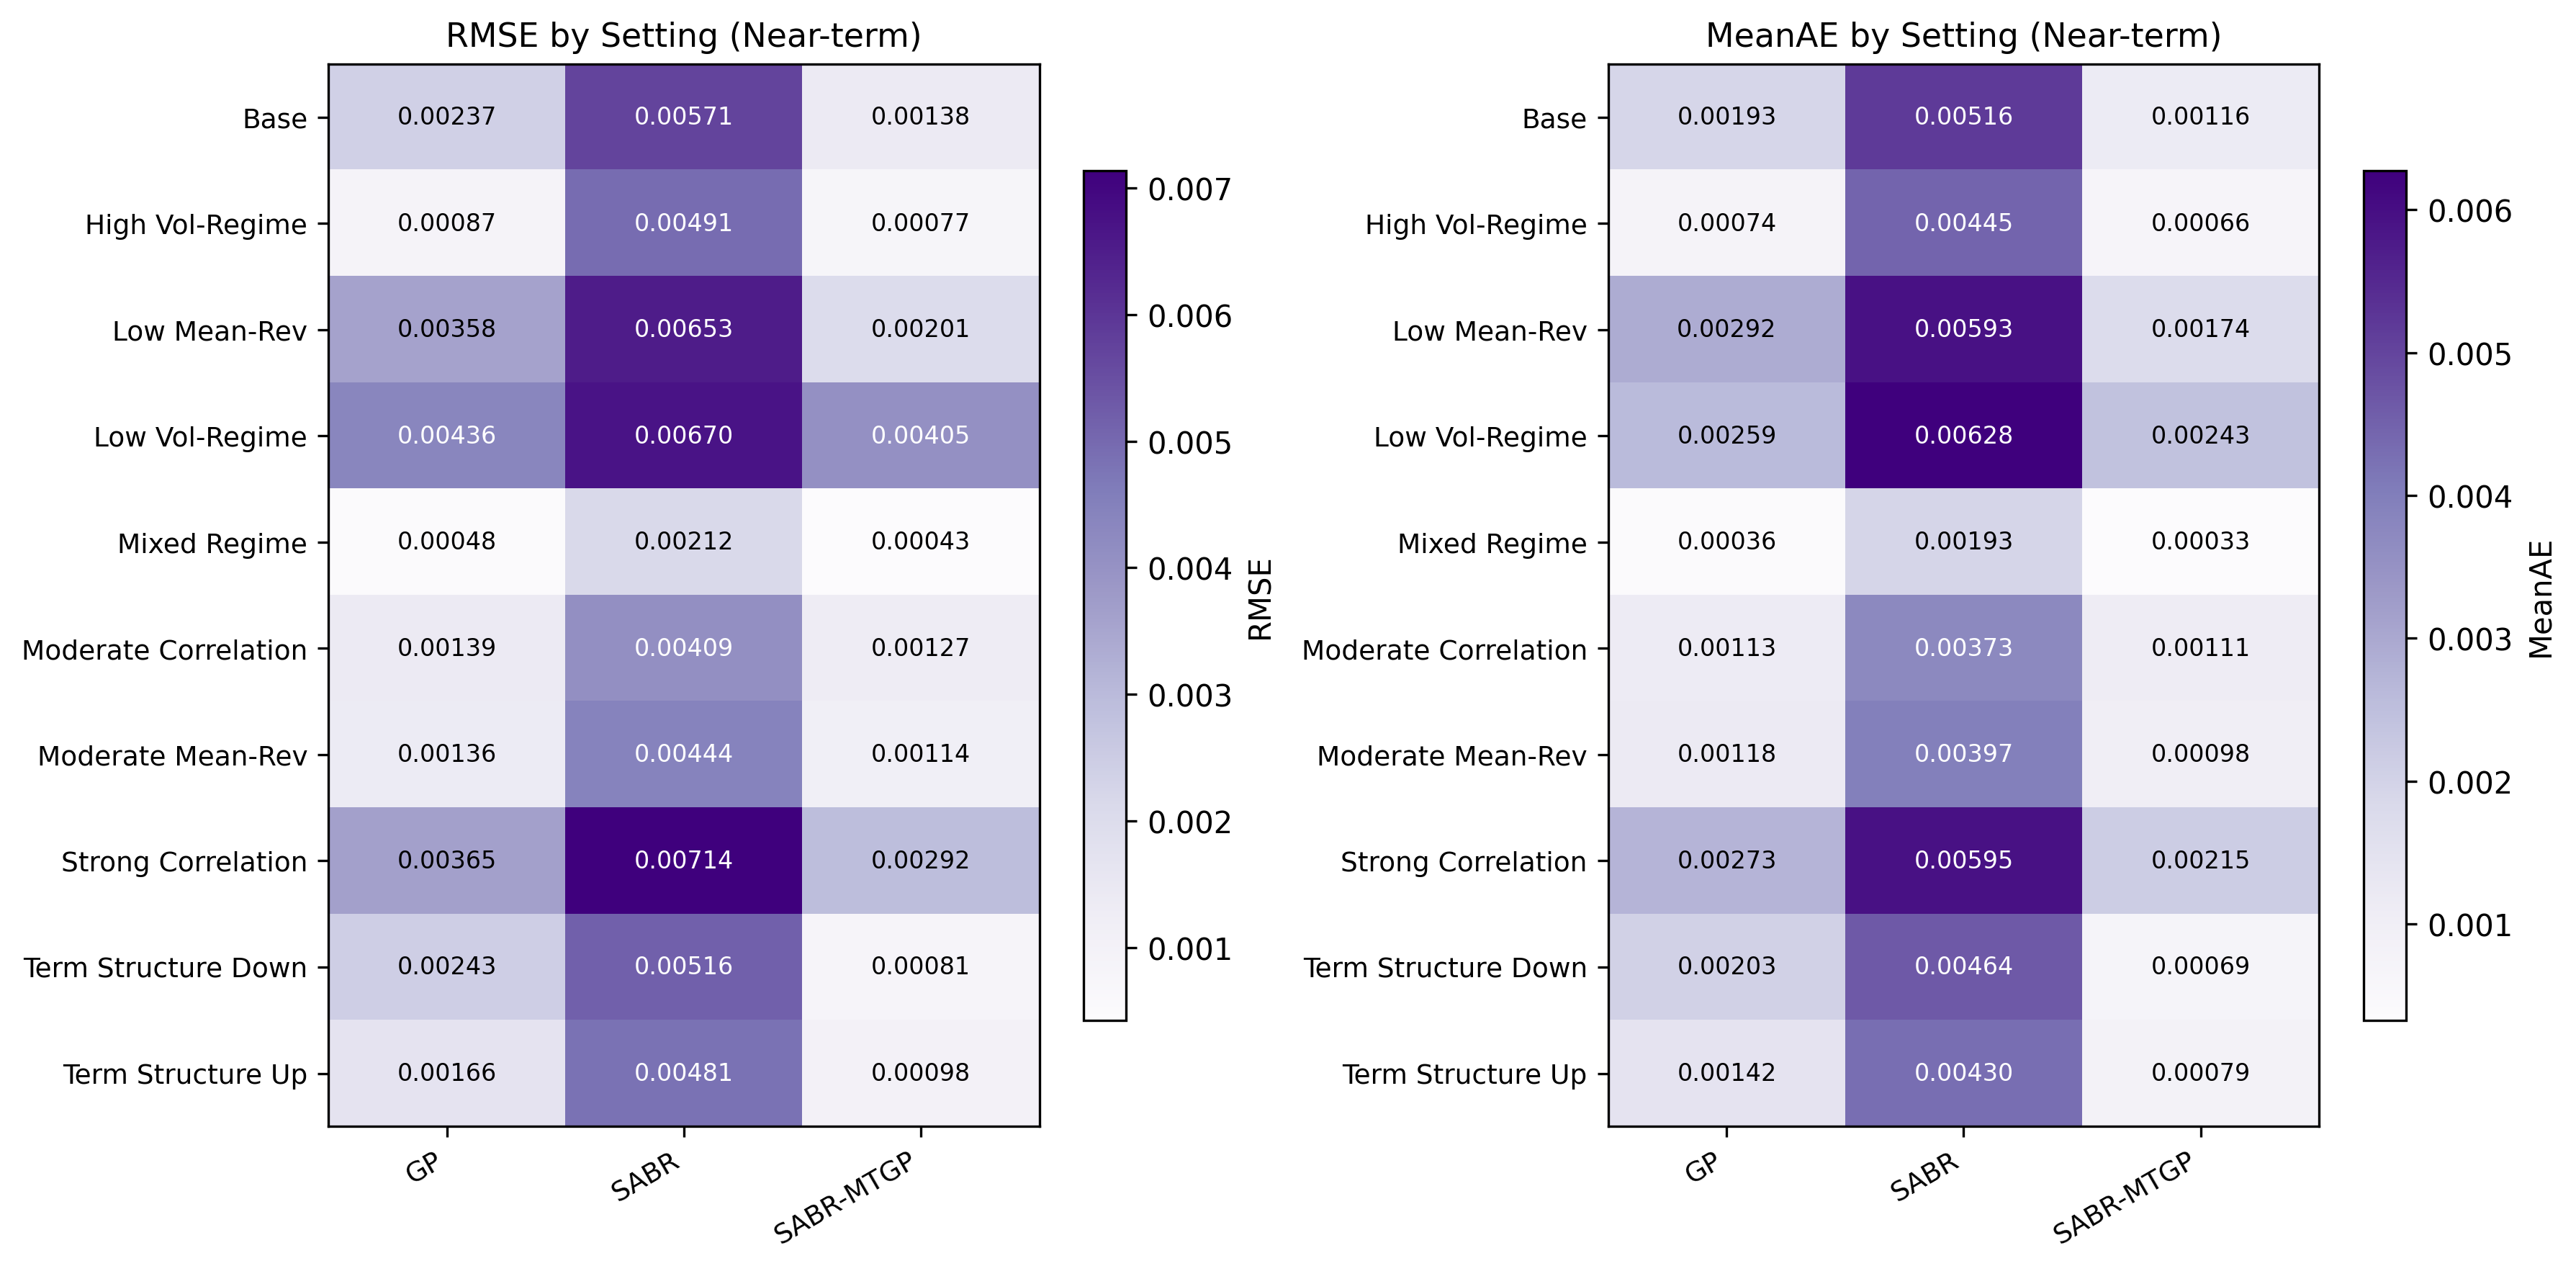
\includegraphics[width=\textwidth]{performance_heatmap_Near-term.png}
    \caption{Performance heatmap (RMSE and MeanAE) across different Heston parameter settings for the Near-term maturity ($\tau=0.3$).}
    \label{fig:heatmap_near}
\end{figure}

\begin{figure}[htbp]
    \centering
    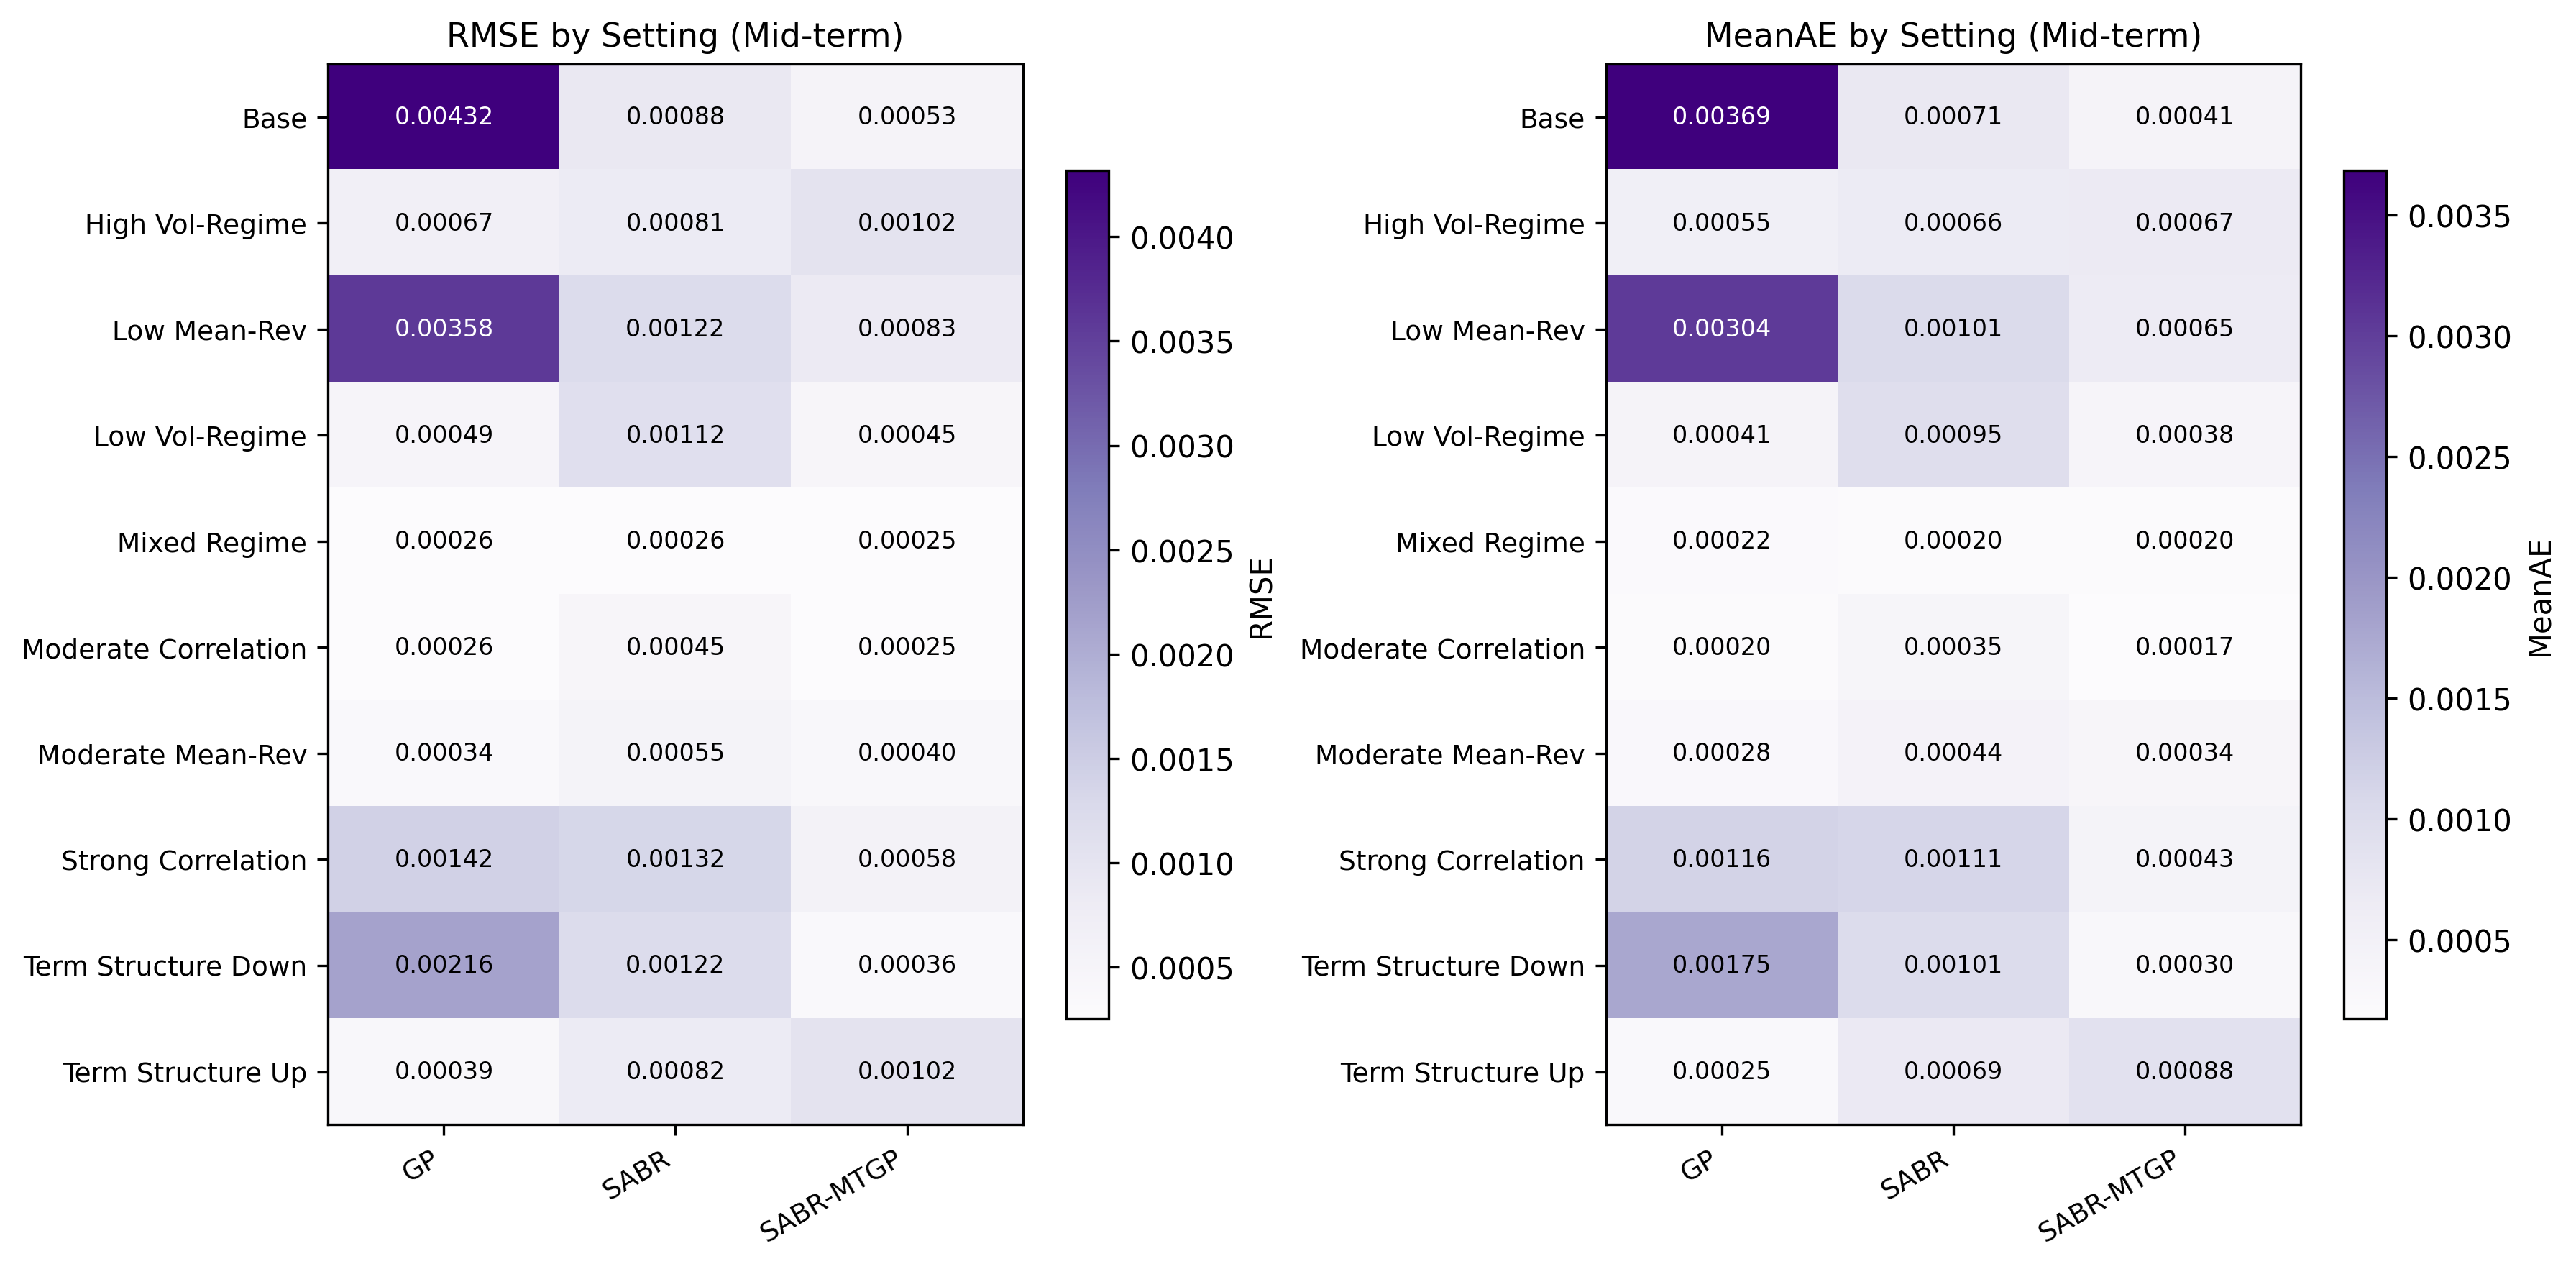
\includegraphics[width=\textwidth]{performance_heatmap_Mid-term.png}
    \caption{Performance heatmap (RMSE and MeanAE) across different Heston parameter settings for the Mid-term maturity ($\tau=0.9$).}
    \label{fig:heatmap_mid}
\end{figure}

\begin{figure}[htbp]
    \centering
    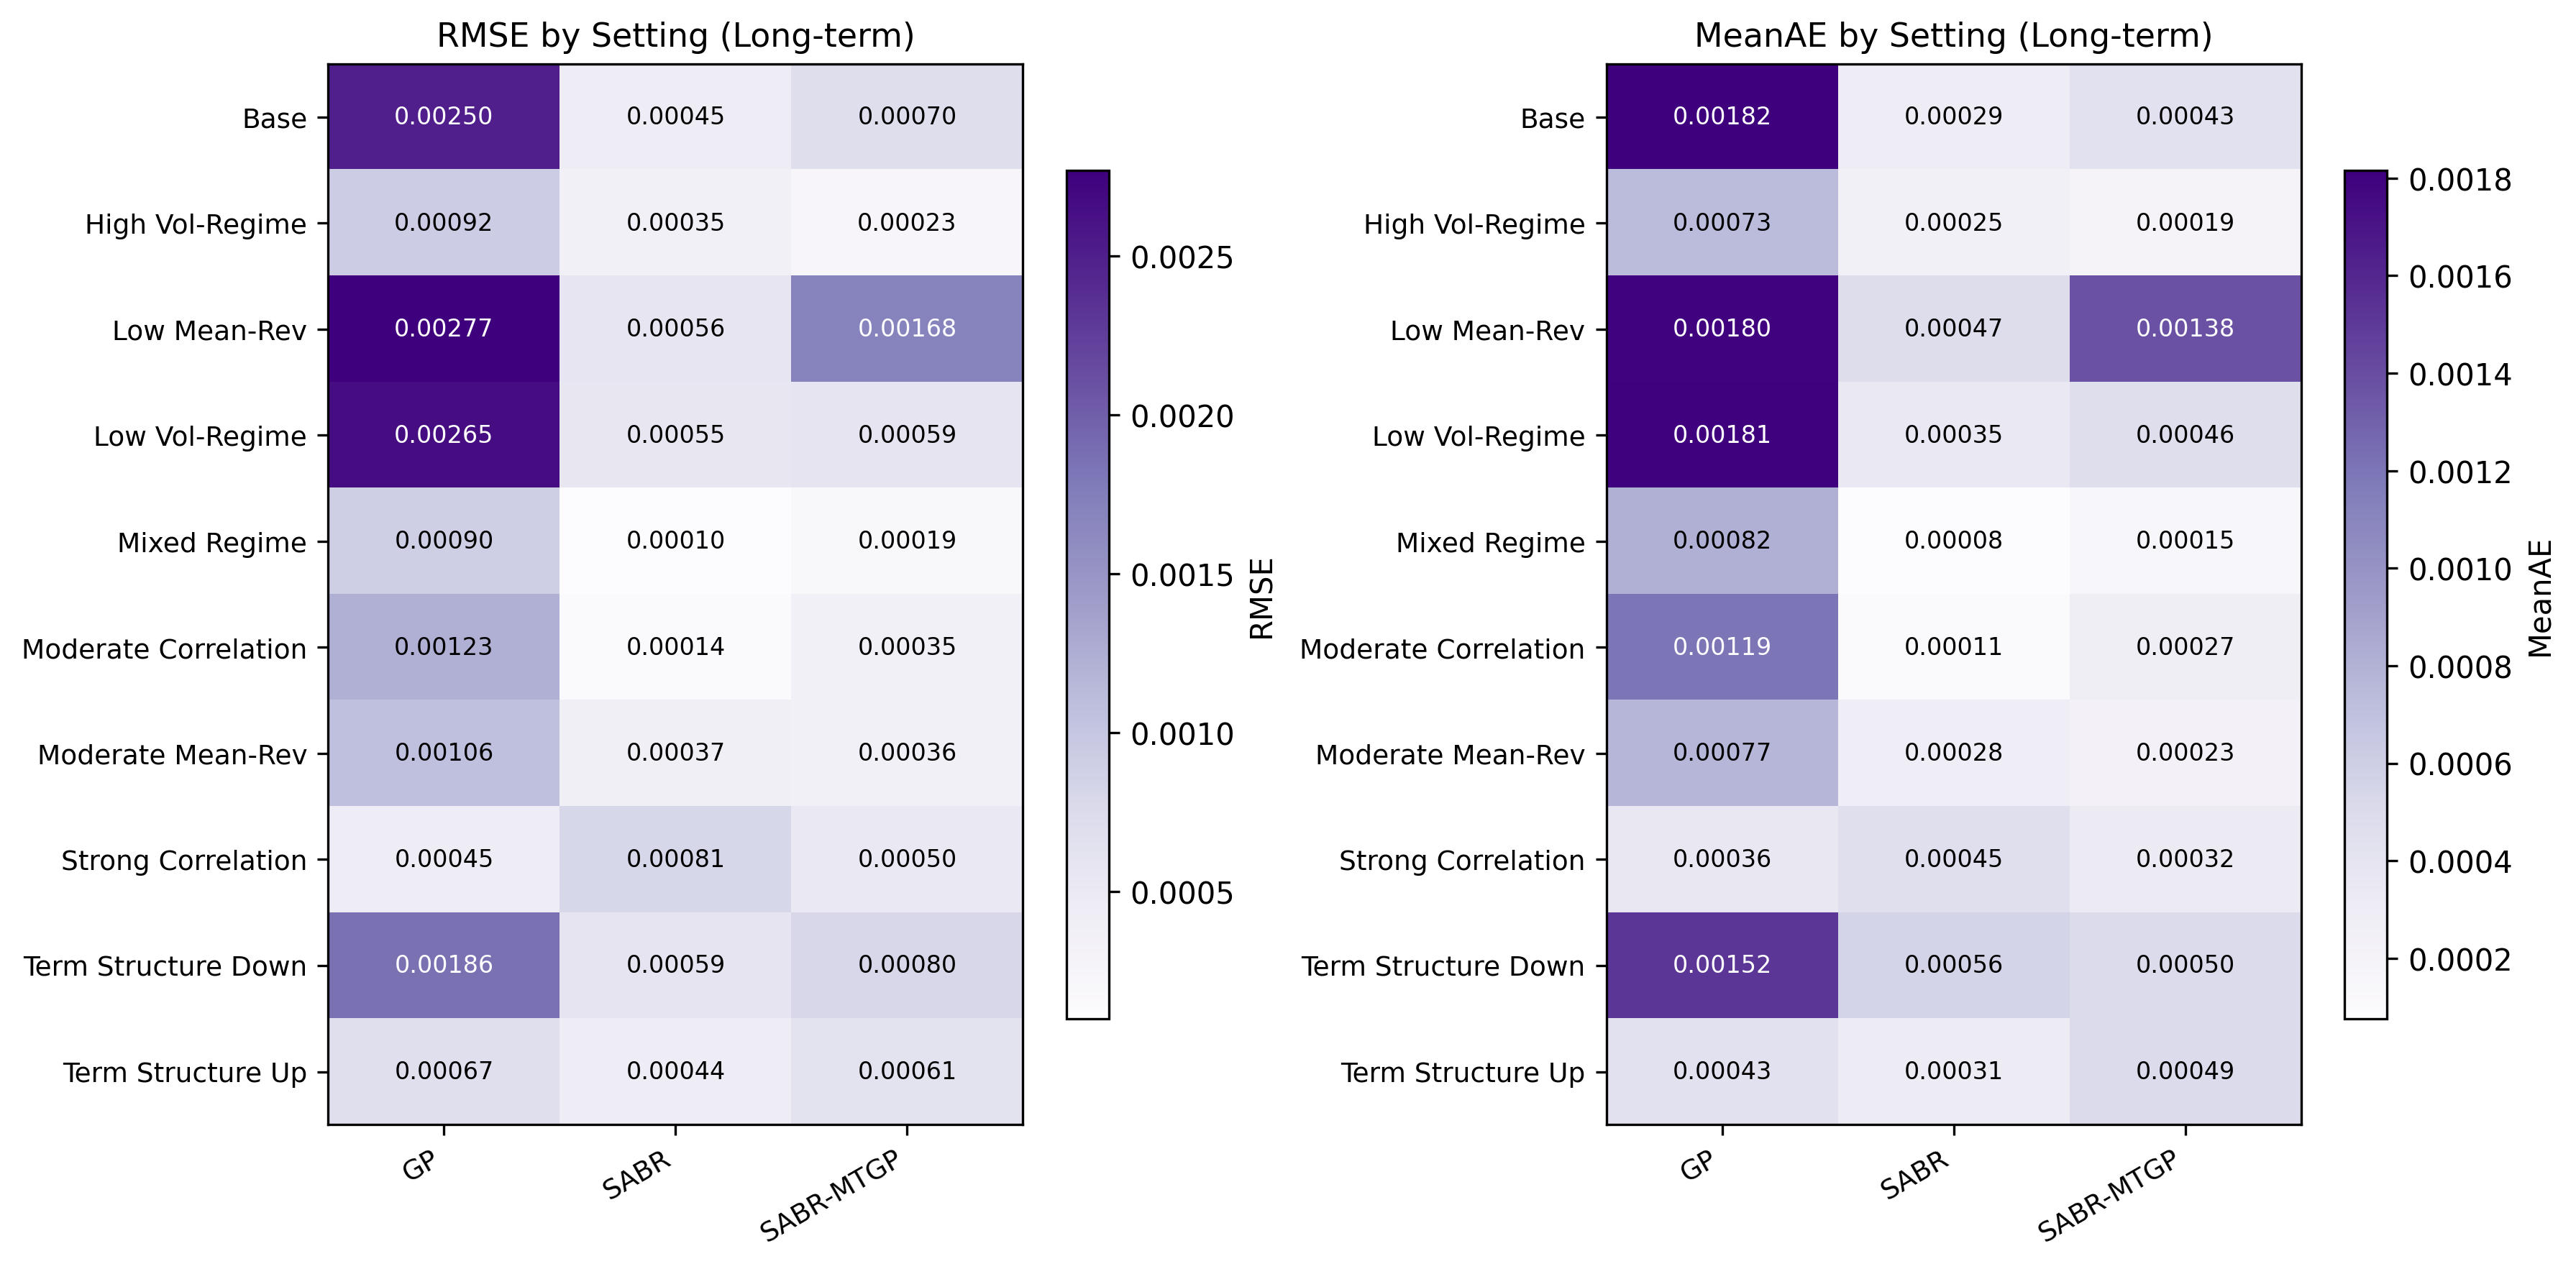
\includegraphics[width=\textwidth]{performance_heatmap_Long-term.png}
    \caption{Performance heatmap (RMSE and MeanAE) across different Heston parameter settings for the Long-term maturity ($\tau=2.2$).}
    \label{fig:heatmap_long}
\end{figure}

These heatmaps show consistent performance patterns. SABR-MTGP consistently demonstrated strong performance, frequently ranking as the best or a very close second-best method. The standard GP showed reasonable performance in the near-term, but its accuracy dropped significantly at long-term maturities, where it yielded the highest errors. Conversely, SABR interpolation struggled in the near-term, often producing the highest errors, but benefited from its fixed structure in long-term cases. It frequently achieved the lowest errors, especially with very sparse data. SABR-MTGP's ability to adaptively blend structural guidance with data-driven flexibility allowed it to maintain high accuracy overall, overcoming SABR's near-term issues and the GP's long-term instability.
\subsection{Learned Task Relationship}

The MTGP framework learned the relationship between the SABR source task and the Heston market target task. Figure~\ref{fig:task_analysis_examples} shows this adaptive relationship for three Heston settings, illustrating variations in learned correlation, covariance structure, and variance decomposition (task-specific proportion $\kappa^2_\mathcal{Z}/(\sigma^2_h+\kappa^2_\mathcal{Z})$ vs. shared variance proportion $\sigma^2_h/(\sigma^2_h+\kappa^2_\mathcal{Z})$).

\begin{figure}[htbp]
    \centering
    % Requires the subcaption package
    \begin{subfigure}[b]{\textwidth}
        \centering
        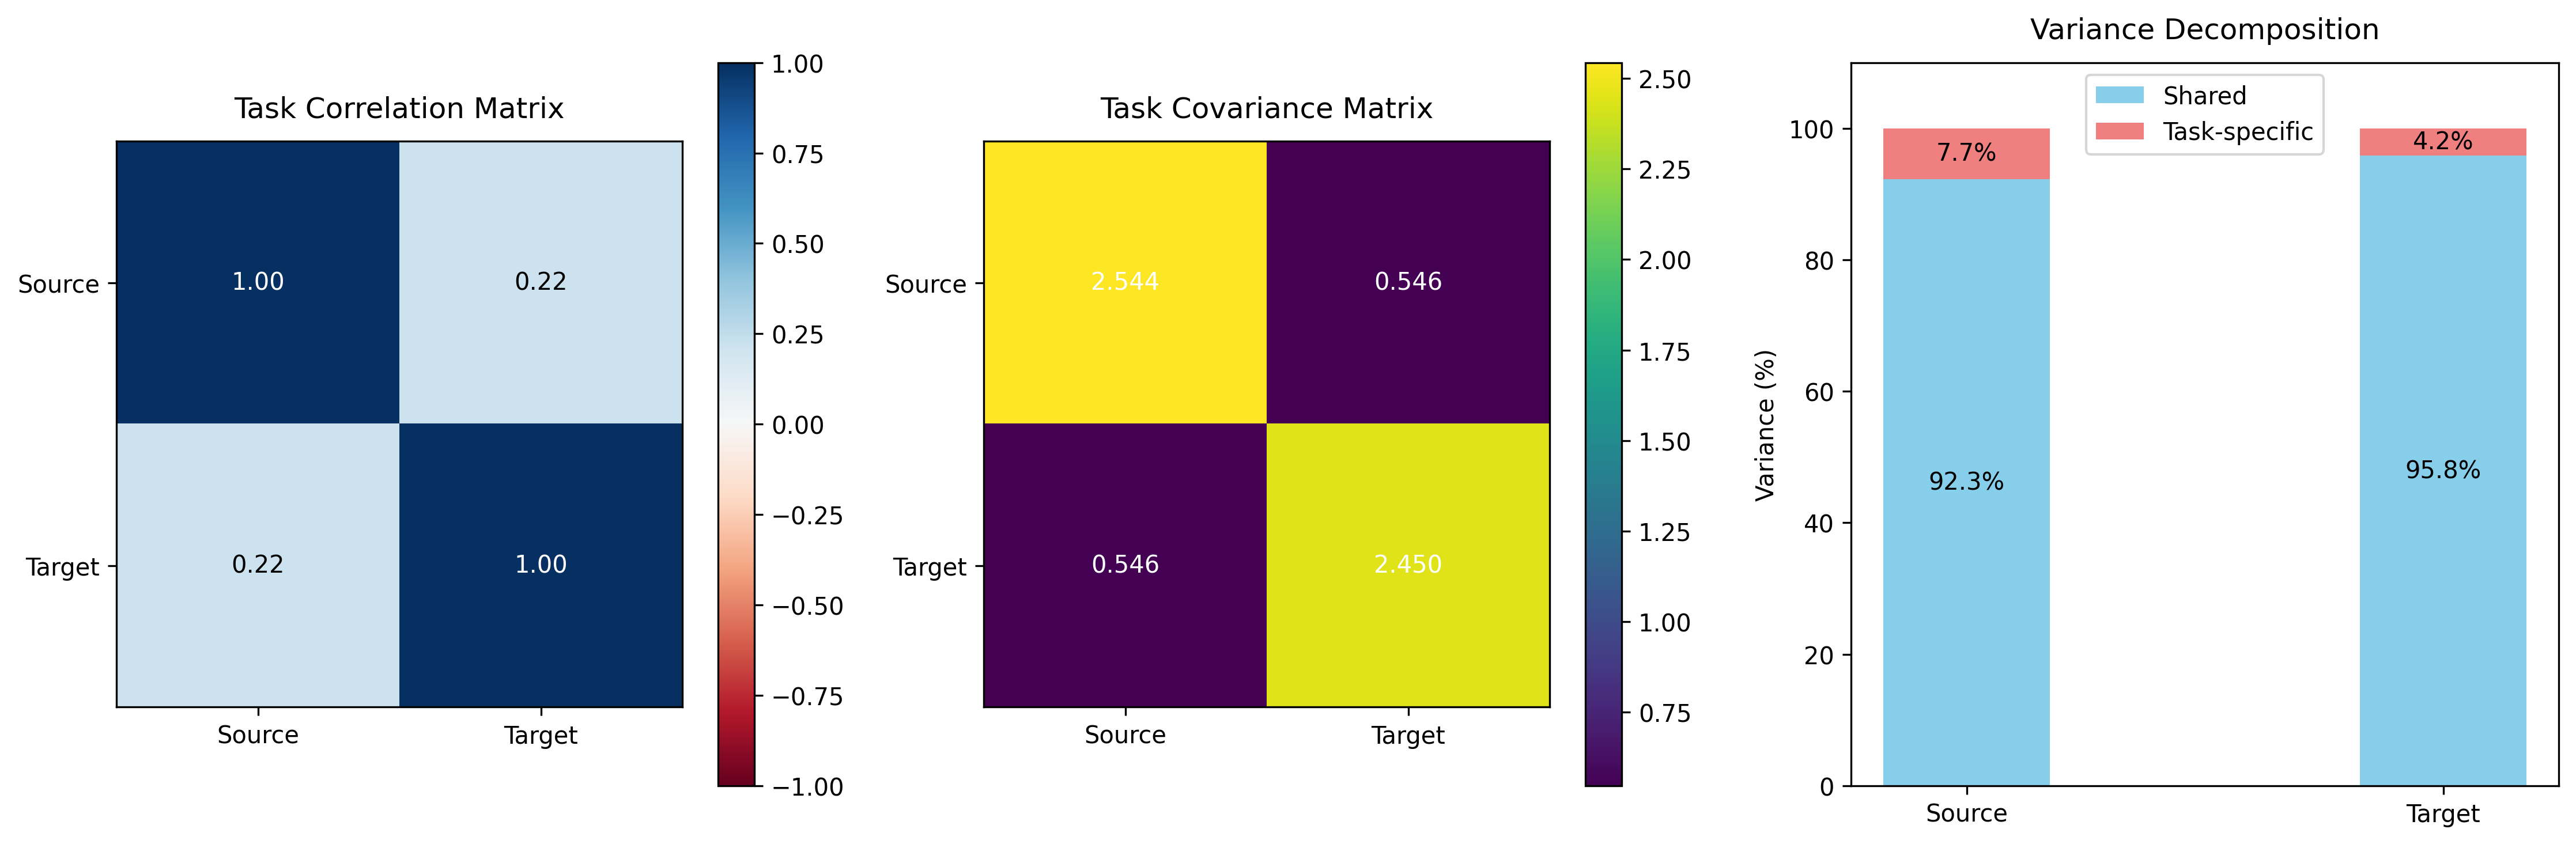
\includegraphics[width=0.9\textwidth]{task_analysis_Moderate_Mean_Rev.png} % Renamed based on mapping
        \caption{Low Correlation Example: \textit{Moderate Mean-Rev} Setting (Learned Correlation = 0.22).}
        \label{fig:task_analysis_low} % Kept label for consistency
    \end{subfigure}
    \vfill % Add vertical space between subfigures
    \begin{subfigure}[b]{\textwidth}
        \centering
        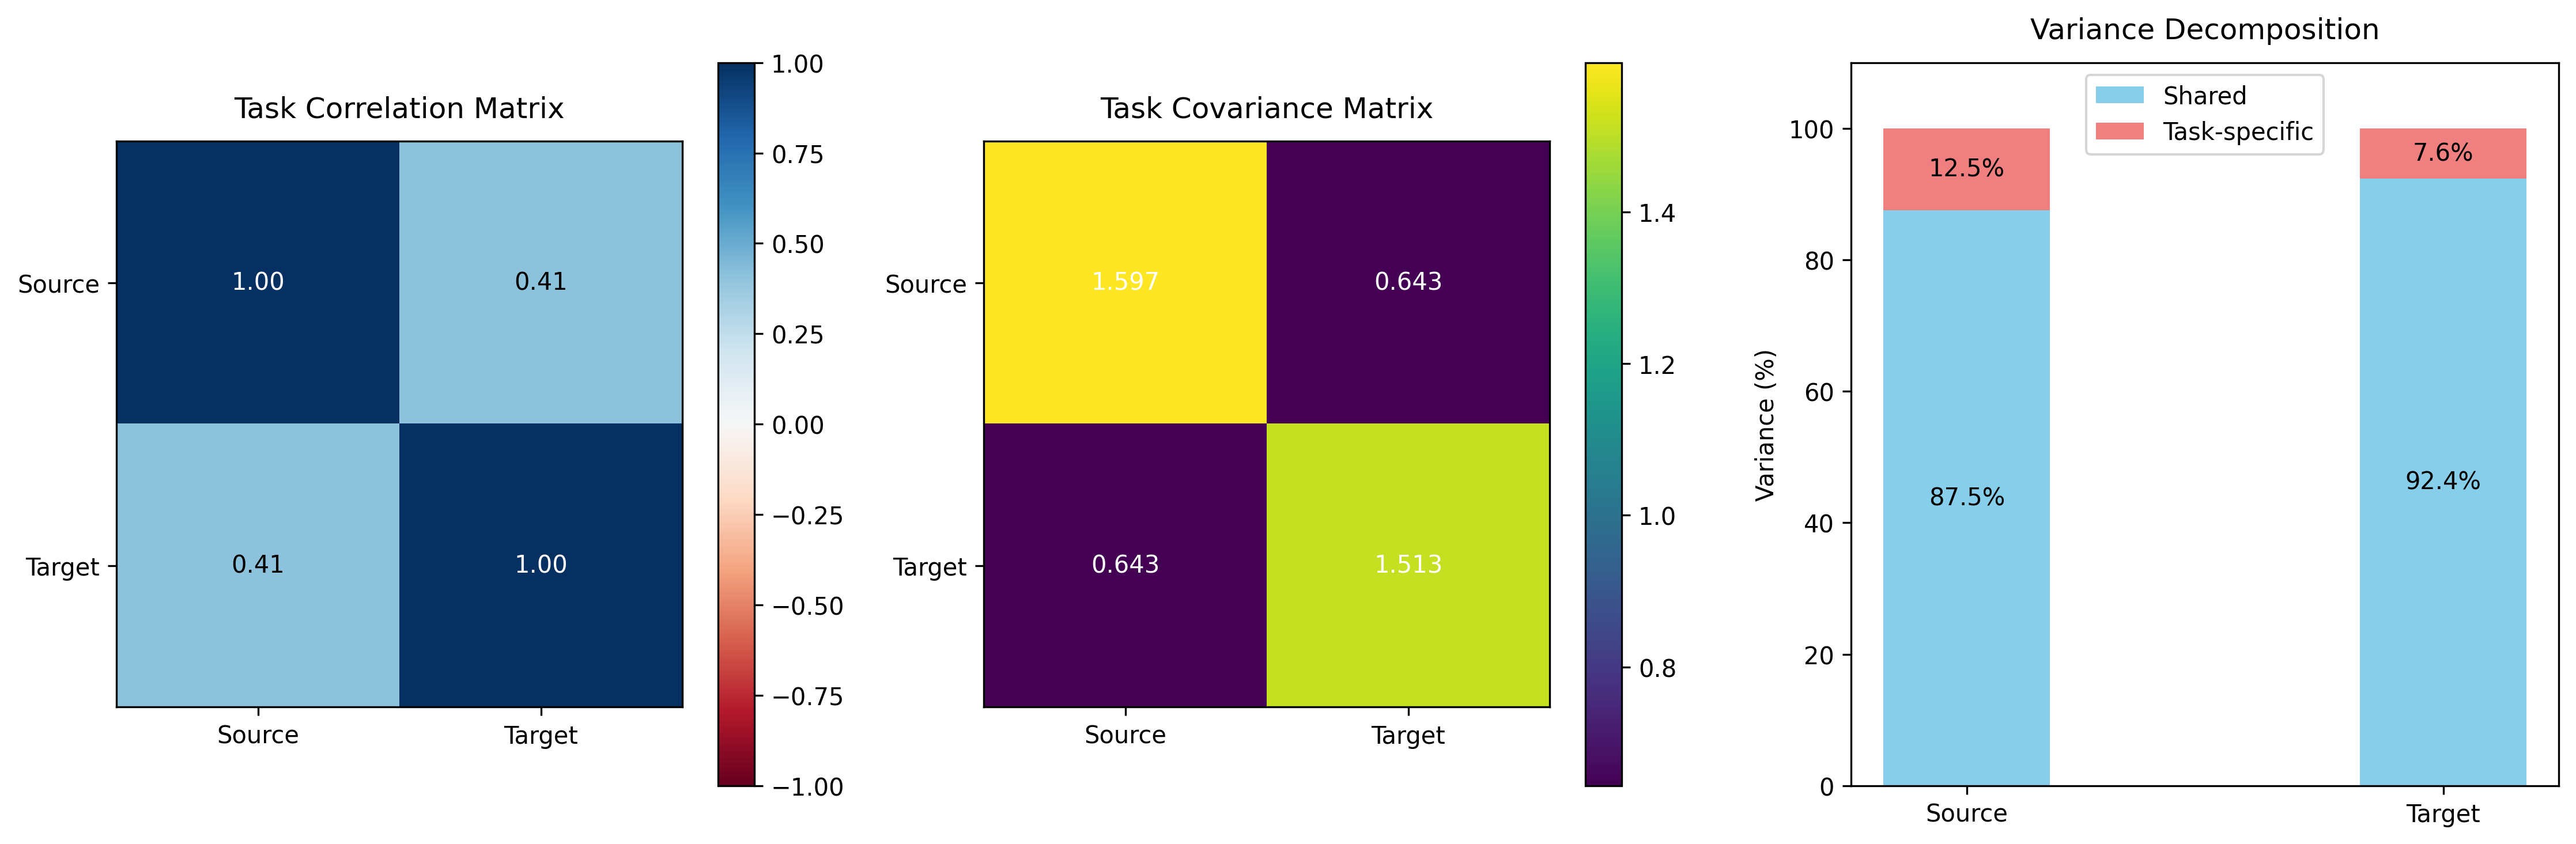
\includegraphics[width=0.9\textwidth]{task_analysis_Base.png} % Renamed based on mapping
        \caption{Moderate Correlation Example: \textit{Base} Setting (Learned Correlation = 0.41).}
        \label{fig:task_analysis_mod} % Kept label for consistency
    \end{subfigure}
    \vfill % Add vertical space between subfigures
    \begin{subfigure}[b]{\textwidth}
        \centering
        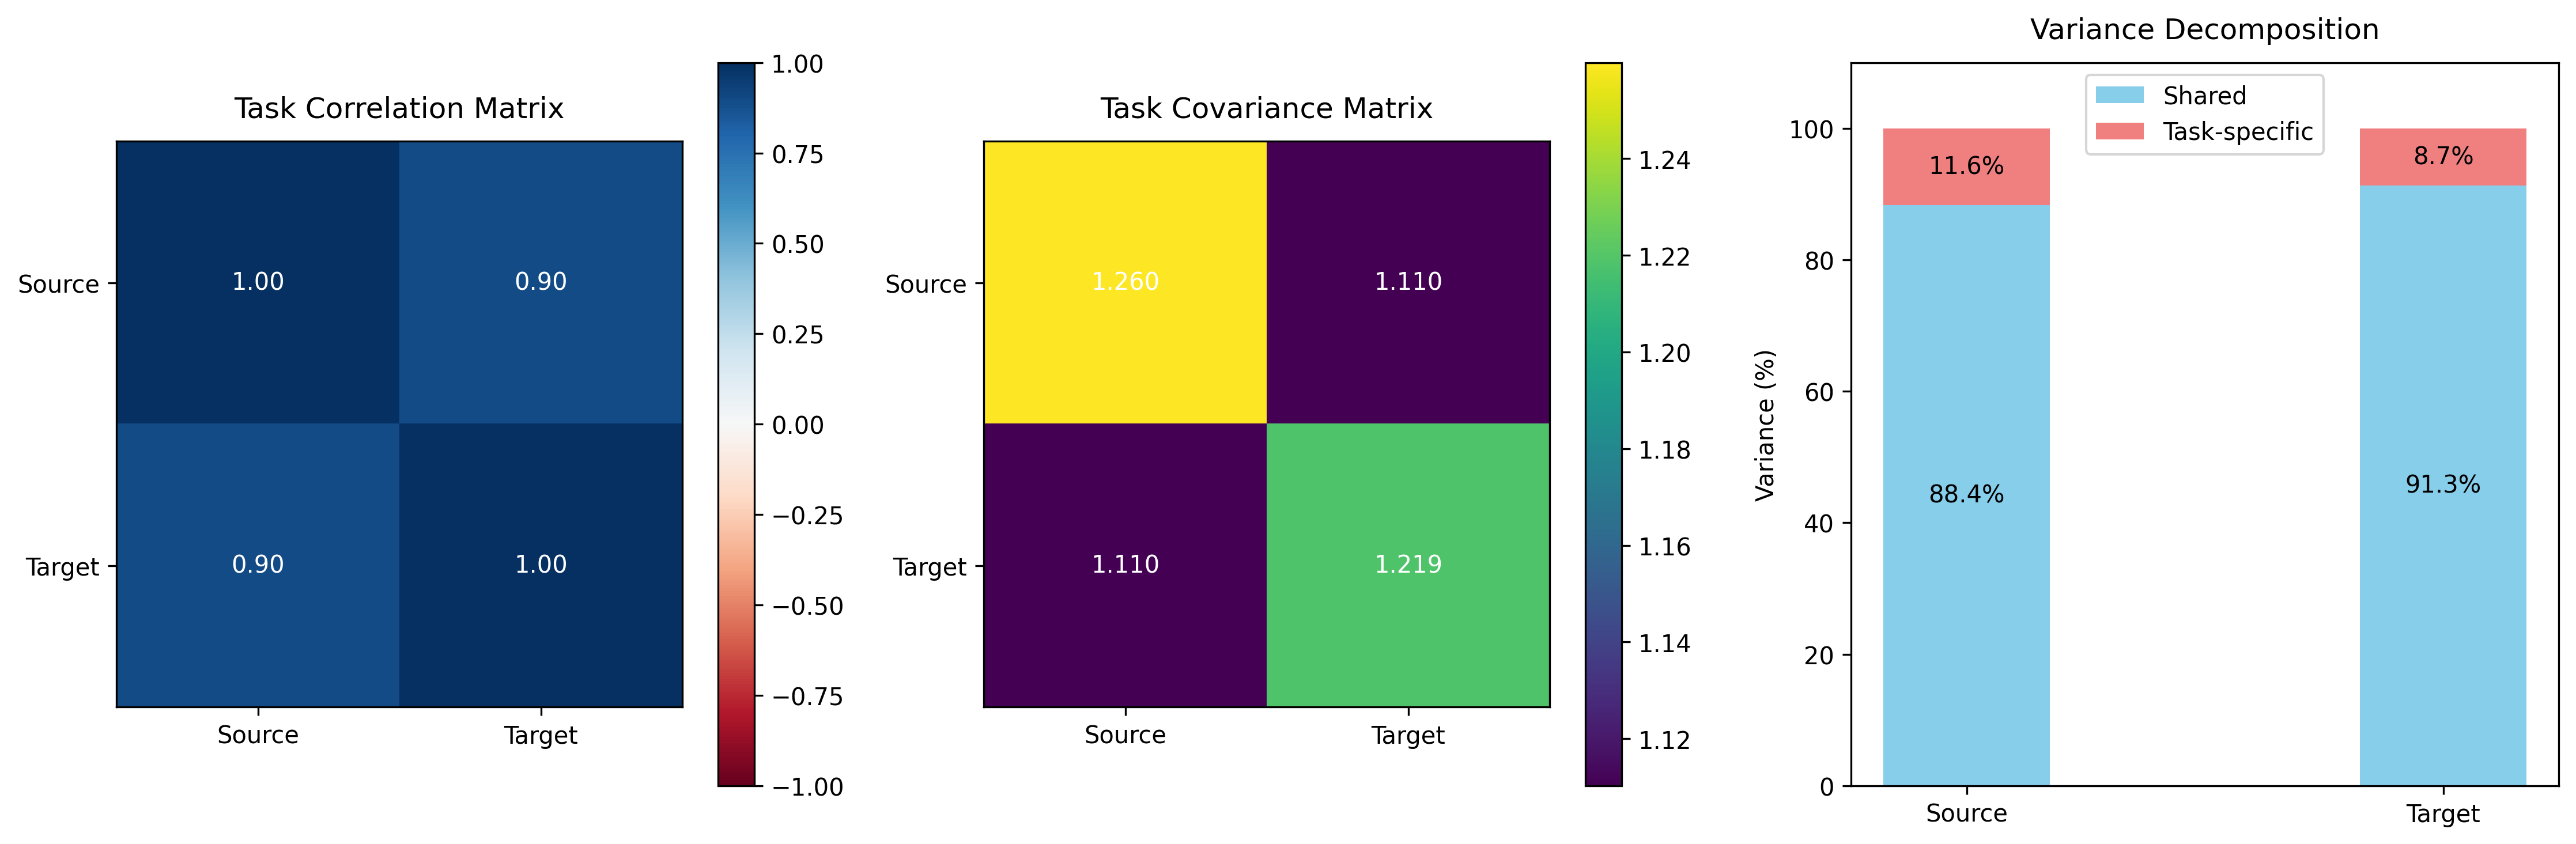
\includegraphics[width=0.9\textwidth]{task_analysis_Term_Structure_Up.png} % Renamed based on mapping
        \caption{High Correlation Example: \textit{Term Structure Up} Setting (Learned Correlation = 0.90).}
        \label{fig:task_analysis_high} % Kept label for consistency
    \end{subfigure}
    \caption{Examples of learned task relationship analysis for the SABR-MTGP model under different Heston parameter settings: (a) \textit{Moderate Mean-Rev}, (b) \textit{Base}, and (c) \textit{Term Structure Up}. Panels show variations in learned correlation (left), covariance structure (center), and variance decomposition (right).}
    \label{fig:task_analysis_examples}
\end{figure}

The learned correlation varied with Heston parameters. Faster mean reversion (\textit{Moderate Mean-Rev}) yielded low correlation (0.22), perhaps because SABR captured these dynamics less well. An upward term structure (\textit{Term Structure Up}) resulted in high correlation (0.90), suggesting SABR provided a better structural approximation in this case. The \textit{Base} setting showed moderate correlation (0.41). This showed the model's ability to assess similarity between SABR information and target data based on market conditions. The task covariance matrices reflected these correlations.

A key pattern was that the shared covariance component consistently accounted for most variance in both tasks across scenarios. Even if SABR is not a perfect match (low correlation), the MTGP leveraged shared properties like smoothness, preventing overfitting to sparse target data and performing better than the standard GP at longer maturities. When SABR aligns well (high correlation), the model strongly used this information, achieving accuracy competitive with or better than SABR interpolation, while maintaining flexibility.

\subsection{Parameter Sensitivity Analysis}

We further examined robustness by analyzing performance sensitivity to Heston parameter changes. Using the coefficient of variation (CV) of RMSE, Figure~\ref{fig:sensitivity_heatmaps} showed how much the precision of each model fluctuated within the parameter categories relative to its average performance. Lower CV (lighter colors) indicated more stable performance.

\begin{figure}[htbp]
    \centering
    % Requires subcaption package
    \begin{subfigure}[b]{\textwidth}
        \centering
        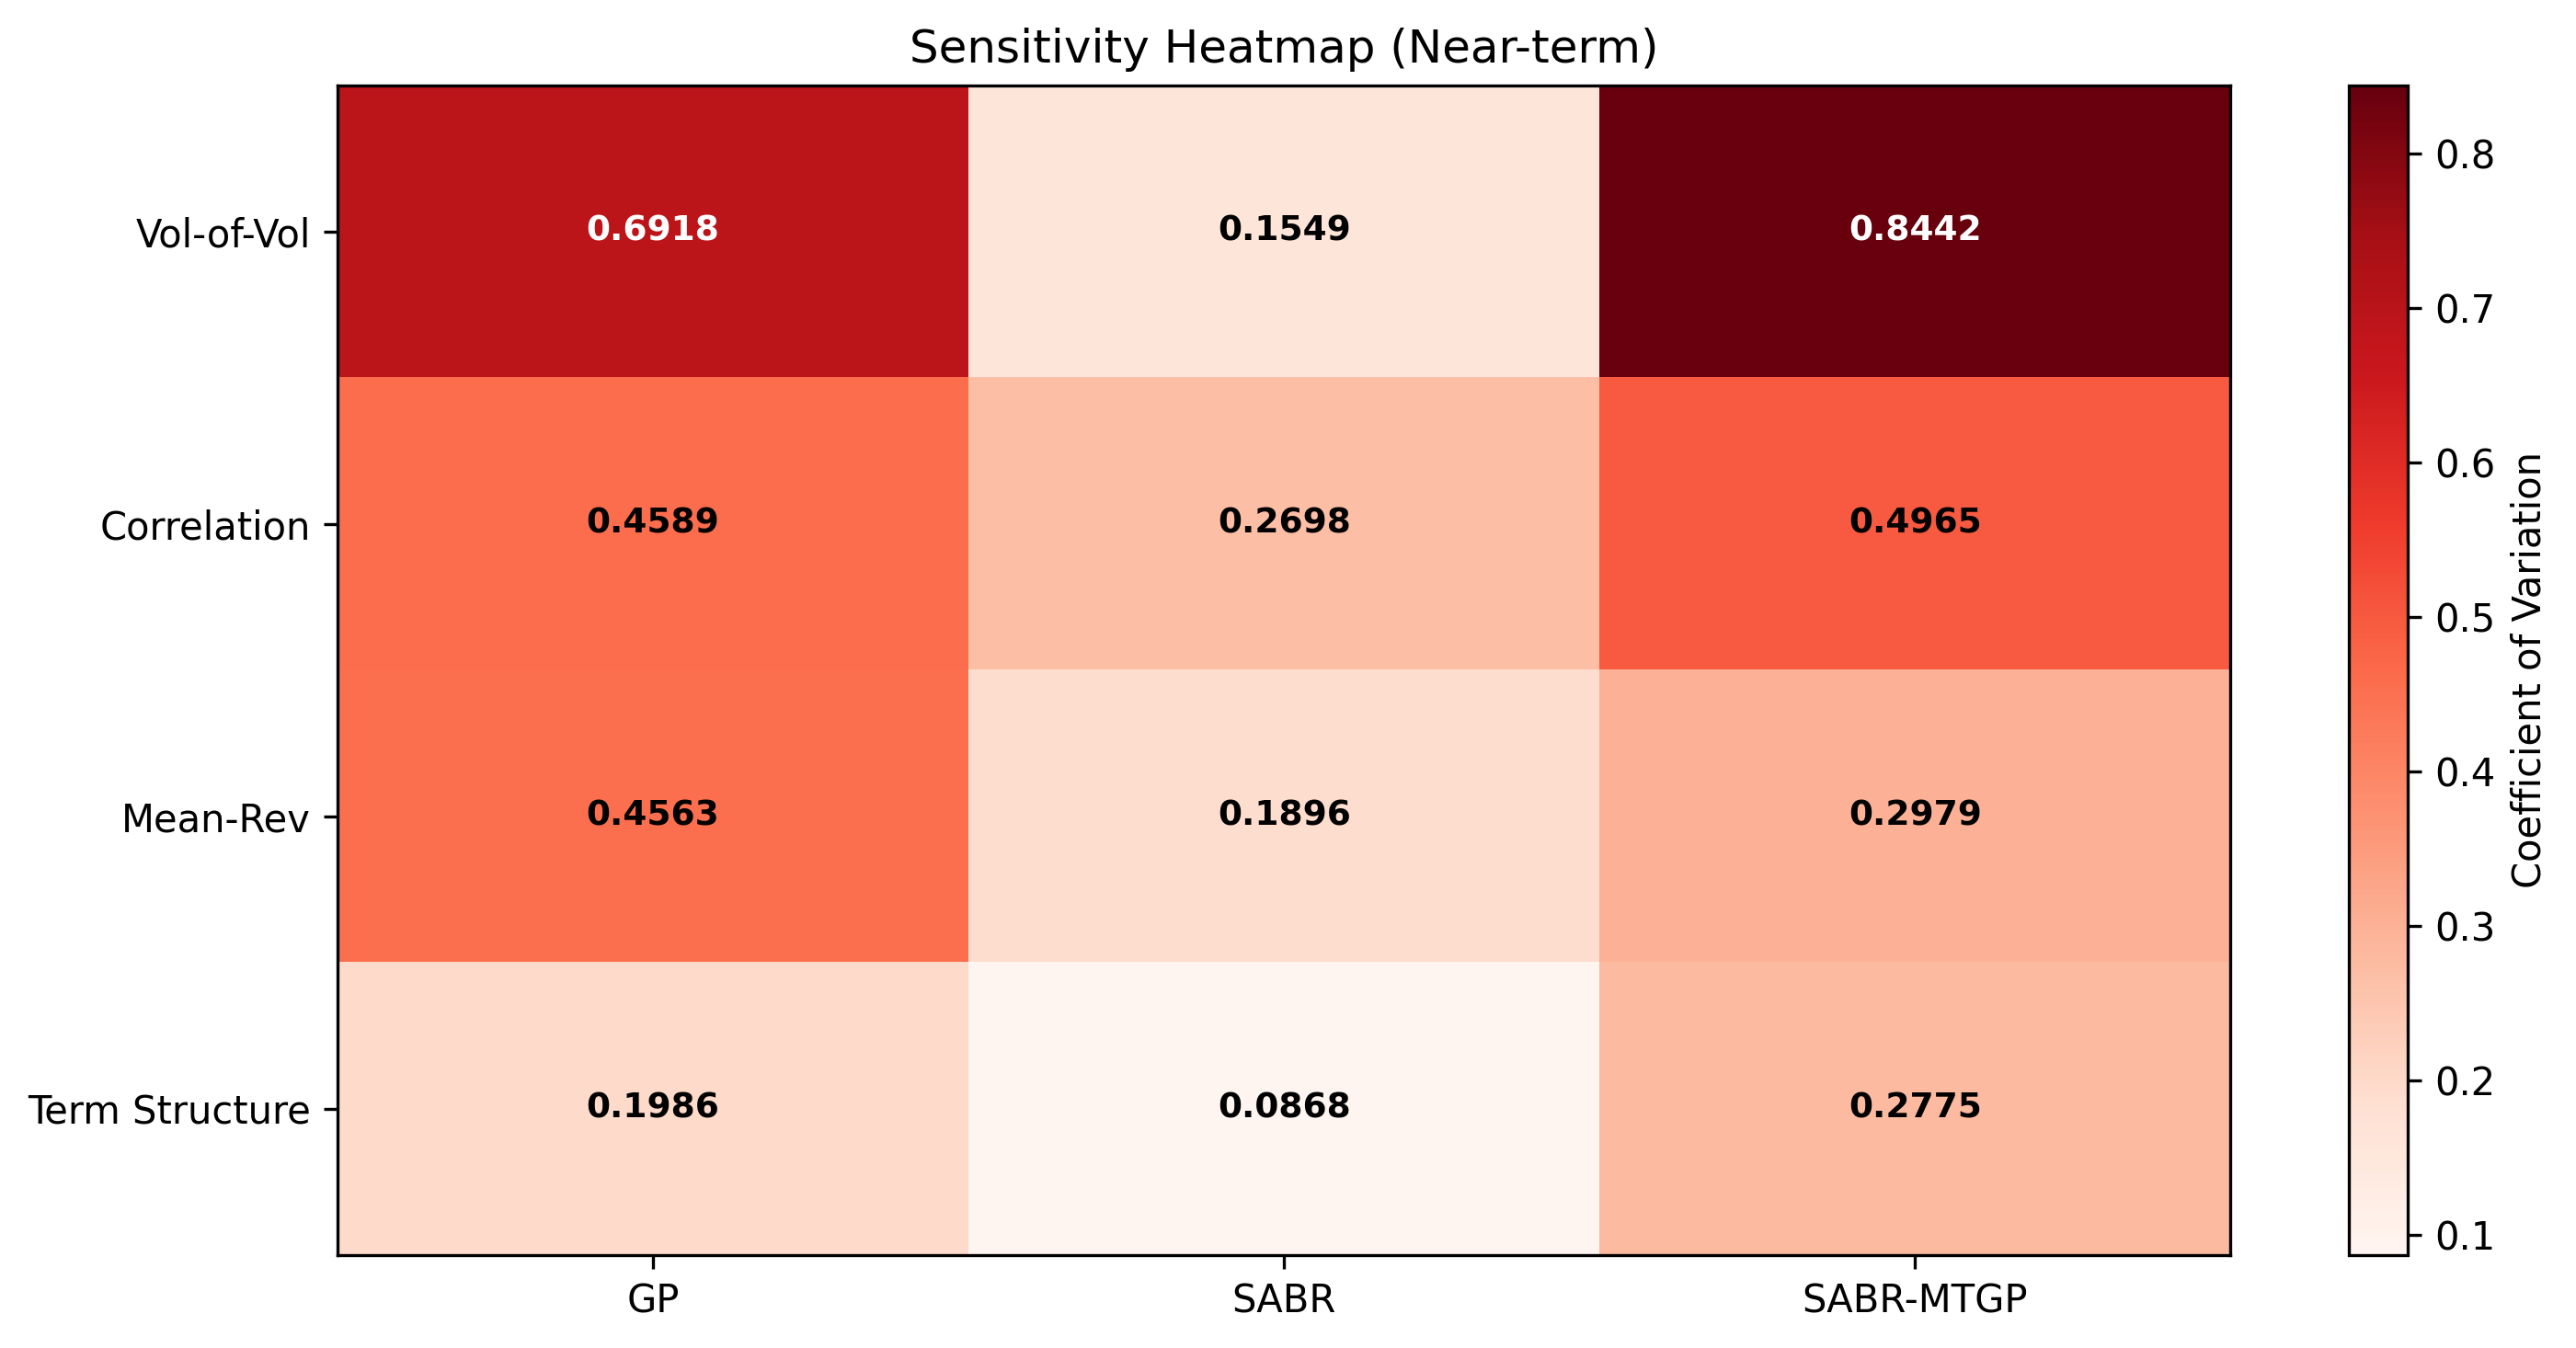
\includegraphics[width=0.75\textwidth]{sensitivity_heatmap_Near-term.png}
        \caption{Near-term ($\tau=0.3$).}
        \label{fig:sensitivity_near}
    \end{subfigure}
    \vfill % Add vertical space
    \begin{subfigure}[b]{\textwidth}
        \centering
        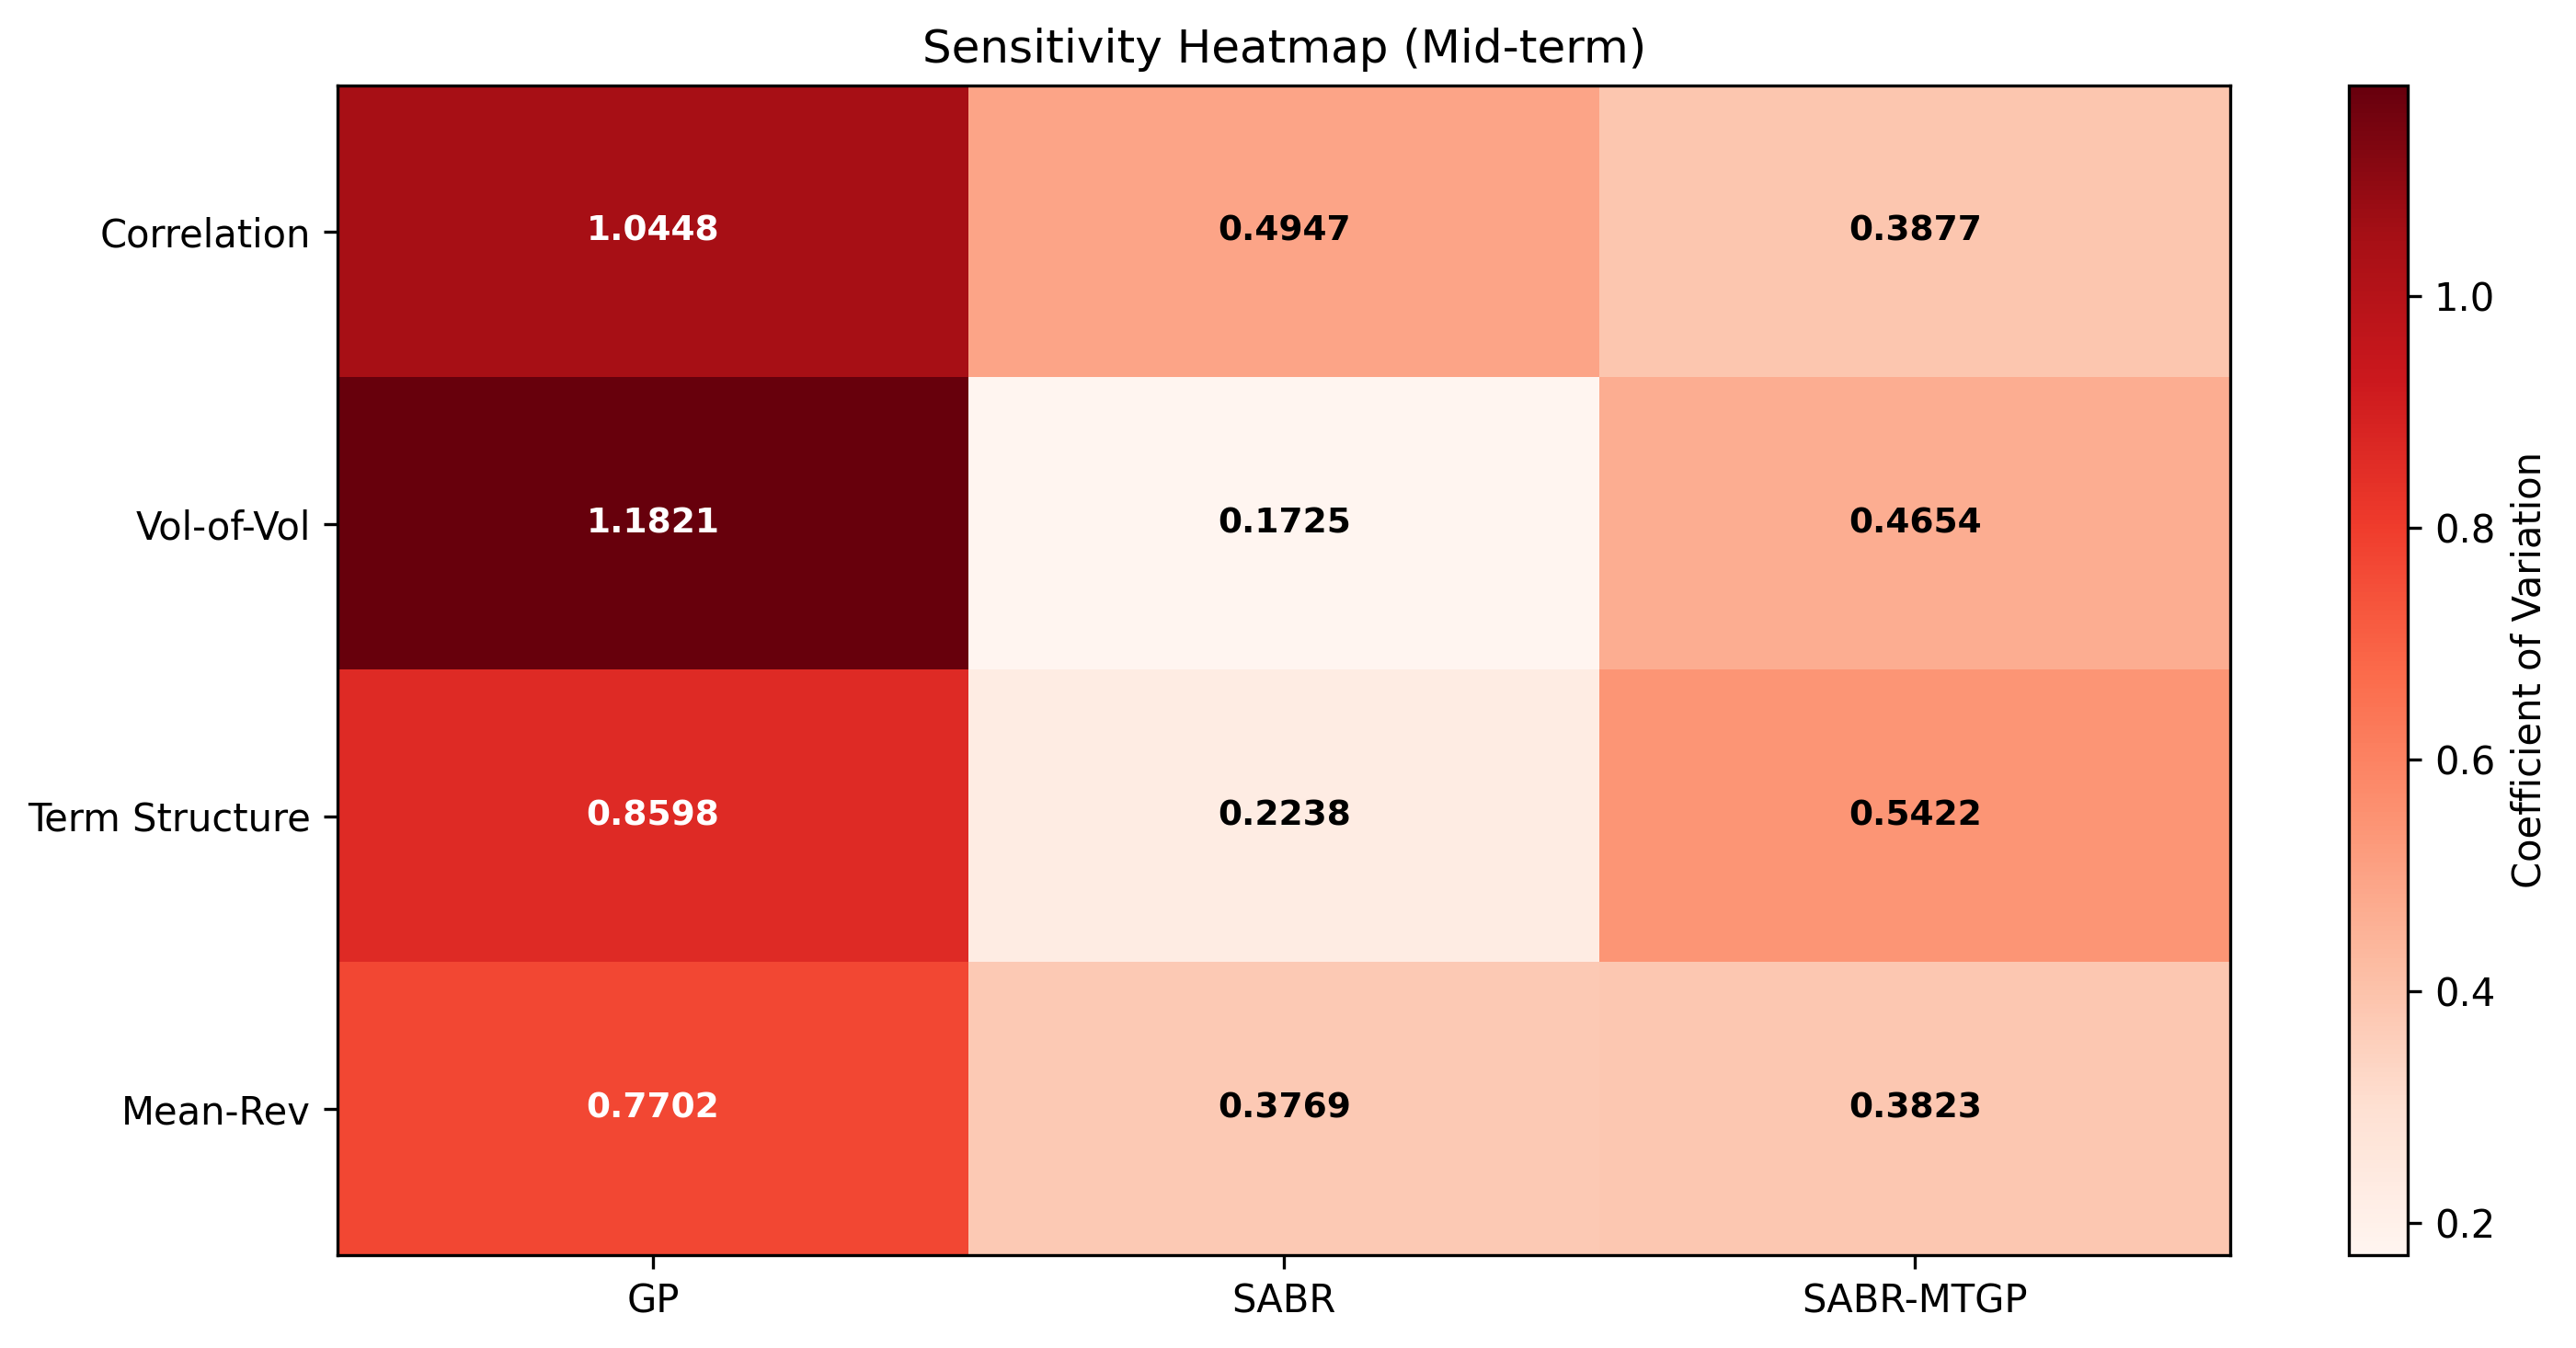
\includegraphics[width=0.75\textwidth]{sensitivity_heatmap_Mid-term.png}
        \caption{Mid-term ($\tau=0.9$).}
        \label{fig:sensitivity_mid}
    \end{subfigure}
    \vfill % Add vertical space
    \begin{subfigure}[b]{\textwidth}
        \centering
        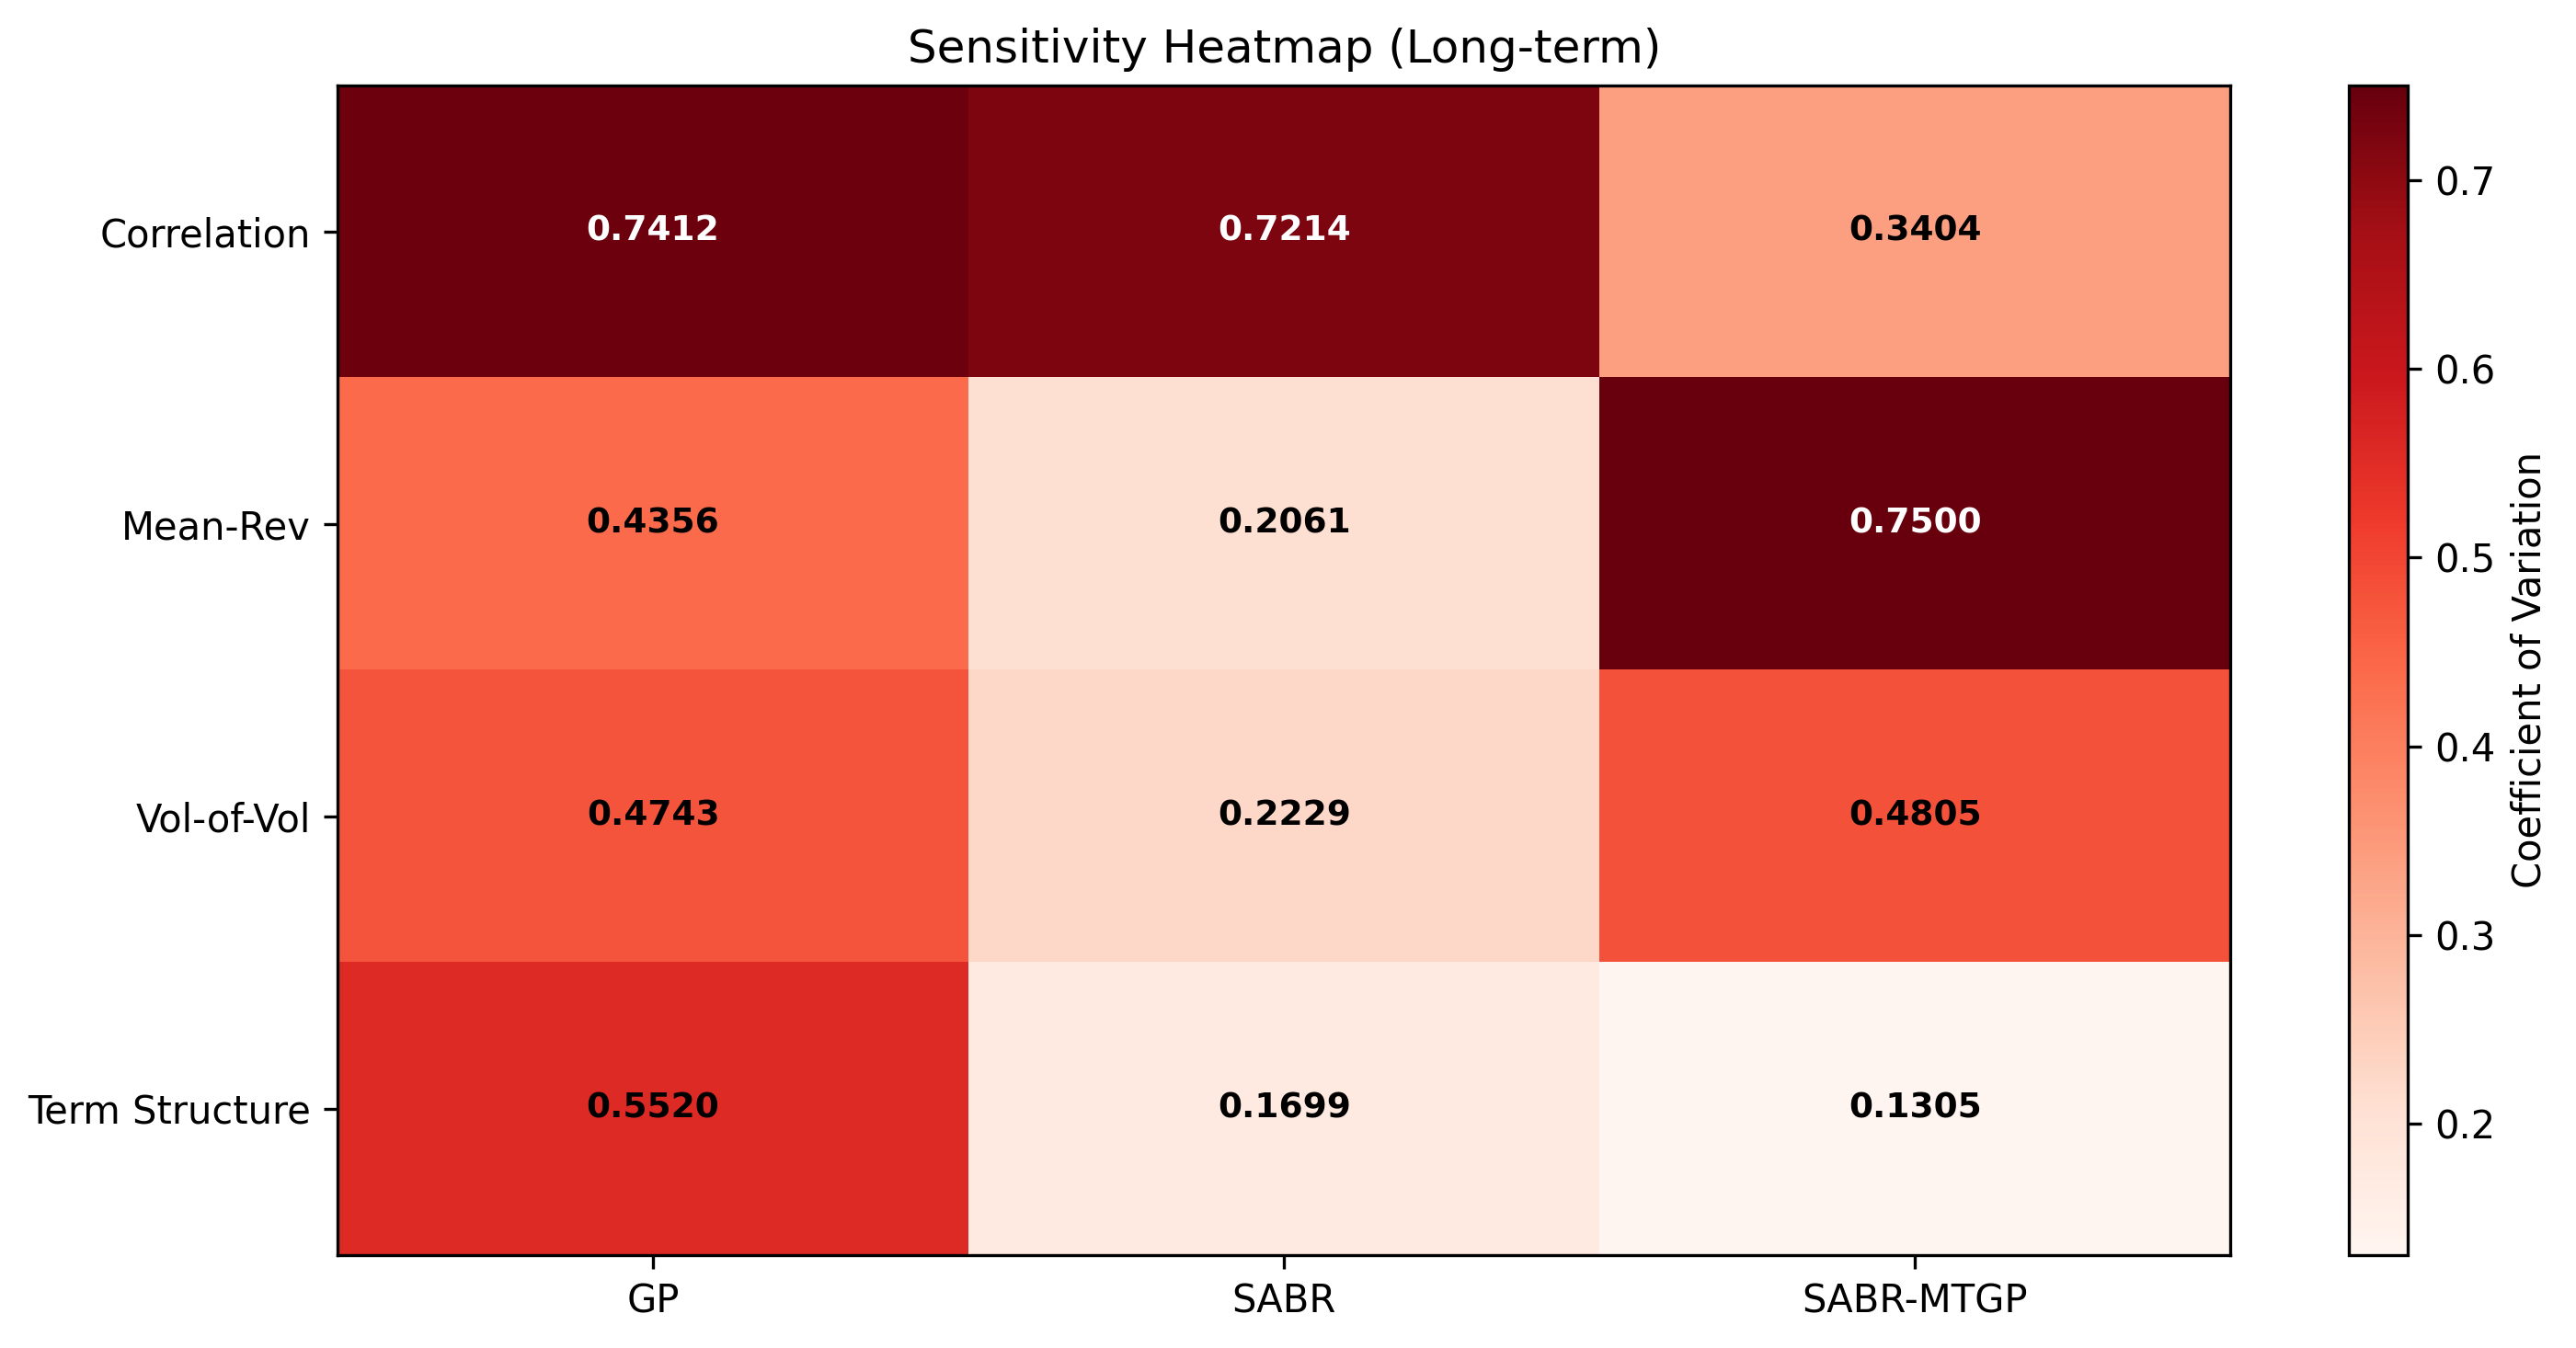
\includegraphics[width=0.75\textwidth]{sensitivity_heatmap_Long-term.png}
        \caption{Long-term ($\tau=2.2$).}
        \label{fig:sensitivity_long}
    \end{subfigure}
    \caption{Parameter sensitivity heatmaps showing the Coefficient of Variation (CV) of RMSE for GP, SABR, and SABR-MTGP across different Heston parameter categories (y-axis) for near-, mid-, and long-term evaluation maturities. Lower CV (lighter color) indicated greater performance stability within that parameter category.}
    \label{fig:sensitivity_heatmaps}
\end{figure}

The sensitivity heatmaps highlighted model stability differences. The standard GP often showed high CV, indicating its performance was sensitive to underlying volatility dynamics, especially concerning `Correlation' and `Vol-of-Vol' changes at longer maturities. SABR interpolation typically had the lowest CV due to its fixed parametric form, but this stability could come at the cost of lower accuracy, particularly near-term. SABR-MTGP generally displayed intermediate stability. It demonstrated improved stability over the standard GP in the mid- and long-term. Although it was less stable than SABR interpolation. The sensitivity results thus complemented accuracy findings: SABR-MTGP found a middle ground, using the prior for improved stability over GP, while retaining adaptive flexibility unlike SABR interpolation.

\subsection{Summary}

The experiments using Heston data suggested SABR-MTGP effectively constructed the IVS. By combining SABR's structural information with market observations in a multi-task framework, it achieved better accuracy and stability than using either a standard GP or SABR. It effectively integrated structural information with observed data, adaptively leveraging SABR insights by assessing their relevance to the target dataset.

\section{Application to SPX Market Data} \label{sec:spx_application}

To further evaluate the practical applicability of SABR-MTGP, we tested its performance on real-world market data for SPX options (provided by the \textit{OptionMetrics} database), observed on August 1, 2023. This case study complements the controlled experiments using the Heston model by assessing the method's behavior under actual market conditions.

\subsection{Data}

The dataset included European call options on the SPX index. We preprocessed the data by filtering for valid quotes, calculating time-to-maturity, and finding implied volatilities from mid-prices. We used the Zero Coupon Bond yield curve as the interest rate curve, and estimated the dividend yield using put-call parity. This gave us several hundred valid market implied volatility observations across different strikes and maturities up to about one year. Key statistics summarizing this dataset are in Table~\ref{tab:spx_data_summary}. This processed market data was the target task ($\mathcal{D}_\mathcal{T}$) for both the SABR-MTGP model.

\begin{table}[htbp]\small % 'h' means here if possible, 't' top, 'b' bottom, 'p' page of floats
    \centering
    \caption{Descriptive Statistics for the Preprocessed SPX Call Option Dataset (August 1, 2023)}
    \label{tab:spx_data_summary}
    \begin{threeparttable}
    {\small % Make table font smaller
        \begin{tabular}{@{}lc@{}}
            \toprule
            Statistic                 & Value \\
            \midrule
            Total Options             & 524 \\
            Unique Maturities         & 12 \\
            Maturity Range (Years)    & [0.0465, 0.9665] \\
            Strike Price Range        & [3300.00, 6600.00] \\
            Implied Volatility Range  & [0.0986, 0.3322] \\
            \midrule
            \multicolumn{2}{c}{Moneyness Distribution (Based on $K/S_0$, $S_0 = 4576.73$)} \\ % Using actual S0 from script
            \midrule
            In-the-Money ($K/S_0 < 0.95$)   & 68 (13.0\%) \\
            At-the-Money ($0.95 \le K/S_0 \le 1.05$) & 289 (55.2\%) \\
            Out-of-the-Money ($K/S_0 > 1.05$)  & 167 (31.9\%) \\
            \bottomrule
        \end{tabular}
    } % End small
        \begin{tablenotes}
            \item Note: Statistics derived from the preprocessed SPX dataset used in this study. The moneyness definition uses $S_0 = 4576.73$.
        \end{tablenotes}
    \end{threeparttable}
\end{table}


\subsection{Results}

We do not have a ground truth IVS for real market data. So, the evaluation used a qualitative assessment of the model fits and the resulting surfaces. Figure~\ref{fig:spx_slices} shows typical implied volatility slices for near-term ($\tau=0.2190$ years) and mid-term ($\tau=0.8898$ years) maturities.

% --- Combined 2D Slice Figure ---
\begin{figure}[htbp]
    \centering
    \begin{subfigure}[b]{\textwidth}
        \centering
        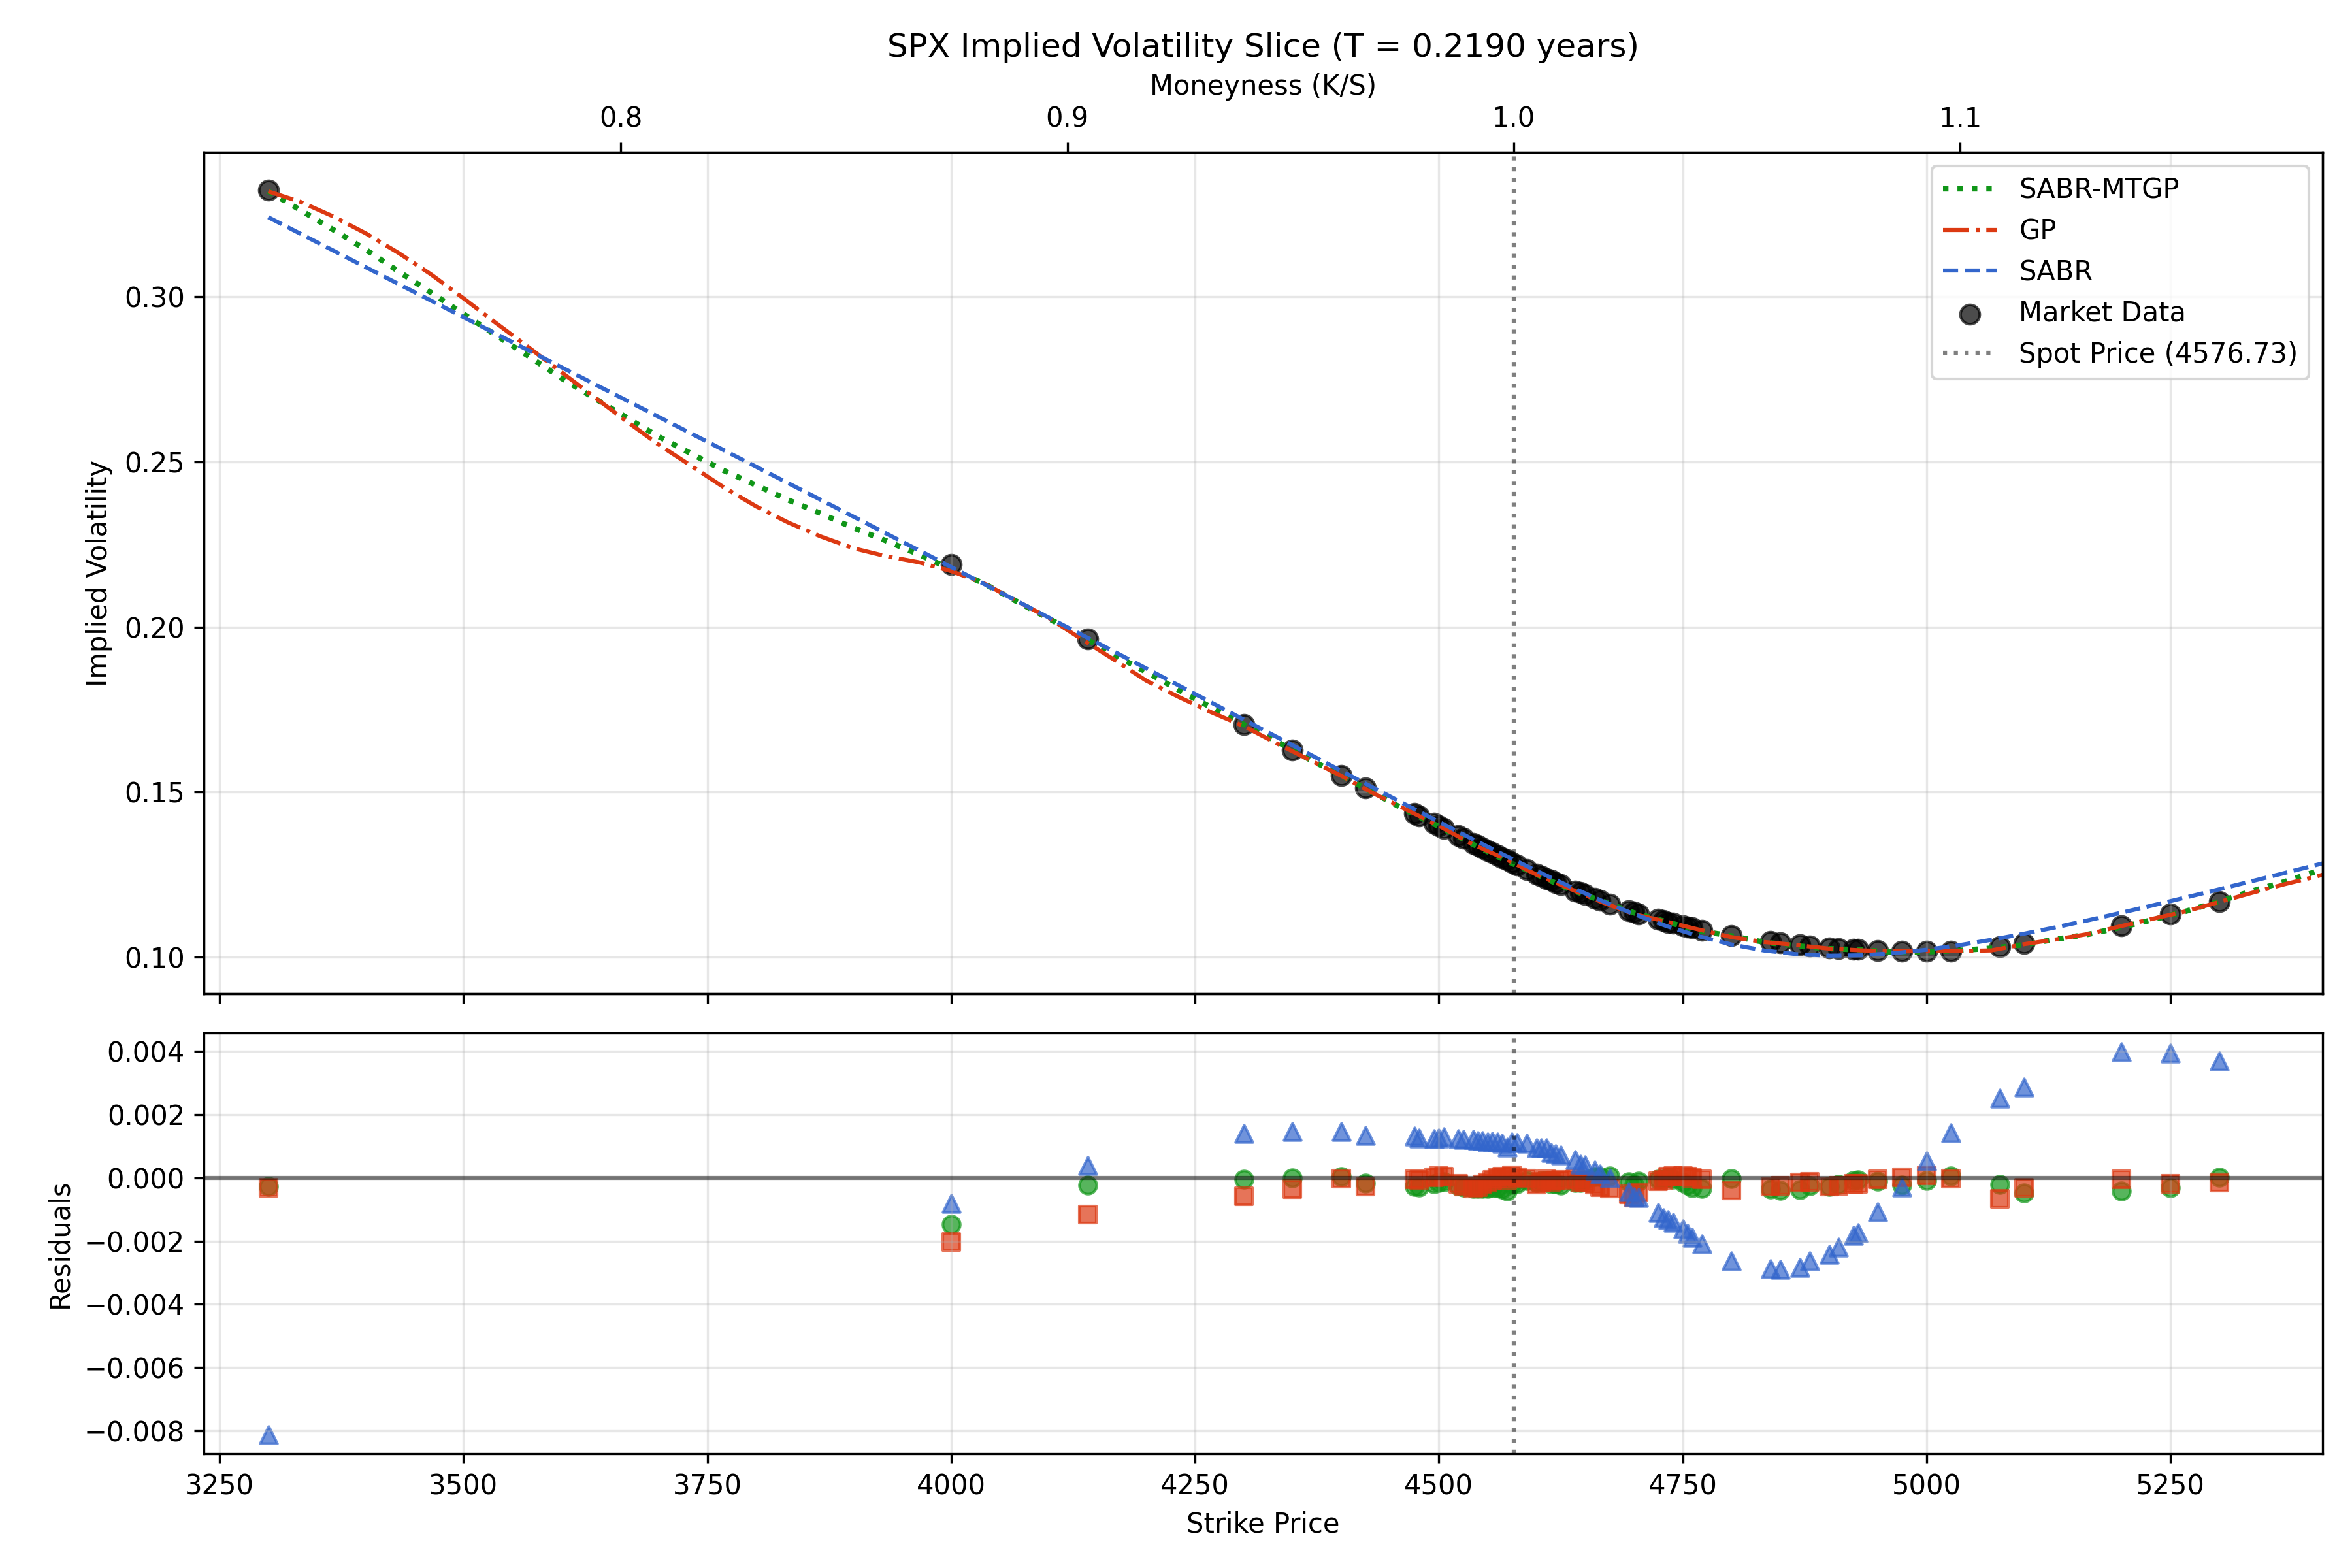
\includegraphics[width=0.9\textwidth]{spx_iv_slice_T0.22.png} % Ensure this file exists
        \caption{Near-term maturity ($\tau = 0.2190$ years).}
        \label{fig:spx_slice_short_sub}
    \end{subfigure}
    \vfill % Add vertical space
    \begin{subfigure}[b]{\textwidth}
        \centering
        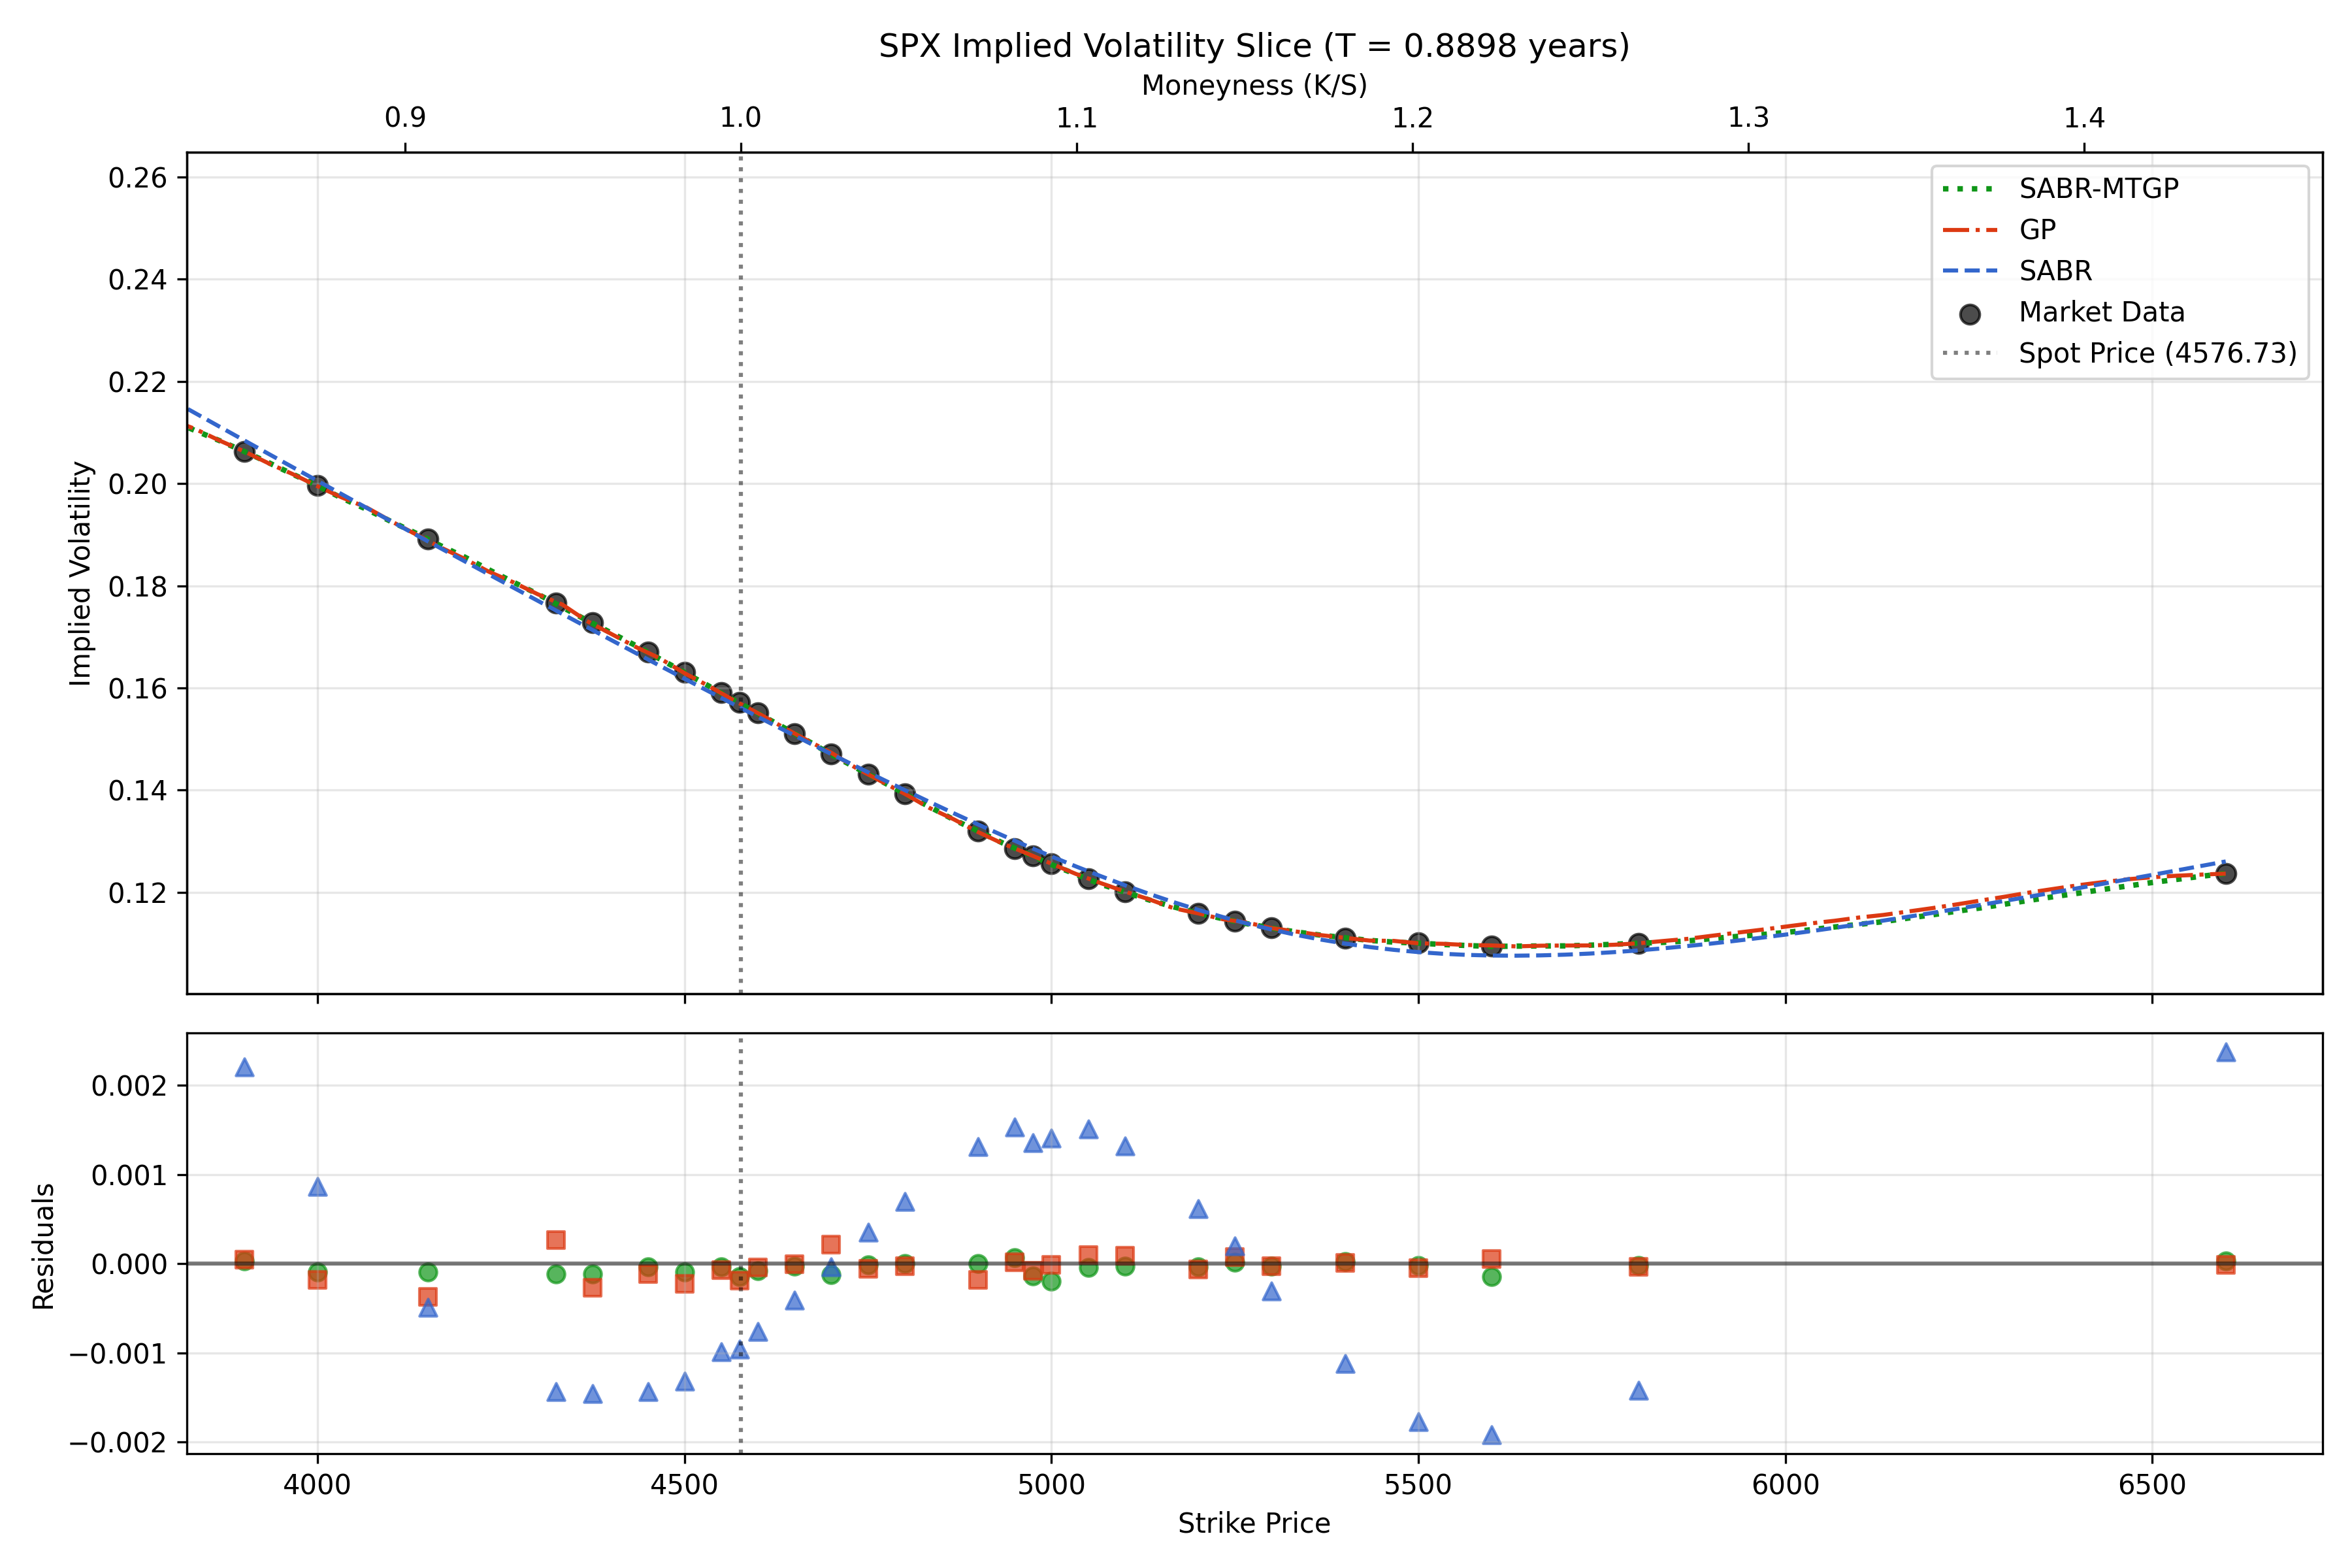
\includegraphics[width=0.9\textwidth]{spx_iv_slice_T0.89.png} % Ensure this file exists
        \caption{Mid-term maturity ($\tau = 0.8898$ years).}
        \label{fig:spx_slice_mid_sub}
    \end{subfigure}
    \caption{Implied volatility slices for SPX options on August 1, 2023. Comparison of SABR-MTGP, GP, and SABR interpolation against market data points. Residuals (Model - Market) are shown below each slice.}
    \label{fig:spx_slices}
\end{figure}


In both slices (Figure~\ref{fig:spx_slices}), all three methods generally captured the observed smile/skew pattern of the market. But the residual plots showed important differences in fit quality. For the near-term slice (Figure~\ref{fig:spx_slice_short_sub}), SABR interpolation had systematic errors. It underestimated volatility for low strikes (ITM) and overestimated near the money. This was shown by the consistent pattern in its residuals. Both the standard GP and SABR-MTGP fitted the observed market points better, especially around the at-the-money region. But there was a notable difference in the deep in-the-money region (strikes 3250-4000). The standard GP curve, although sloping downward, showed a shape considered less regular and potentially less financially realistic compared to volatility curve given by the SABR. The SABR-MTGP curve maintained a smoother, decreasing volatility in this data-sparse region. This produced a more financially realistic interpolation, likely because of the structural guidance from the SABR source task. For the mid-term slice (Figure~\ref{fig:spx_slice_mid_sub}), where the smile was flatter and the market data was denser, all models achieved a very good fit. Notably, the SABR model fit improved significantly compared to the near-term slice. The residuals for both GP and SABR-MTGP were particularly small (generally within +/- 0.001), demonstrating excellent agreement with market observations.


% --- Combined 3D Surface Figures ---
\begin{figure}[htbp]
    \centering
    \begin{subfigure}[b]{0.32\textwidth}
        \centering
        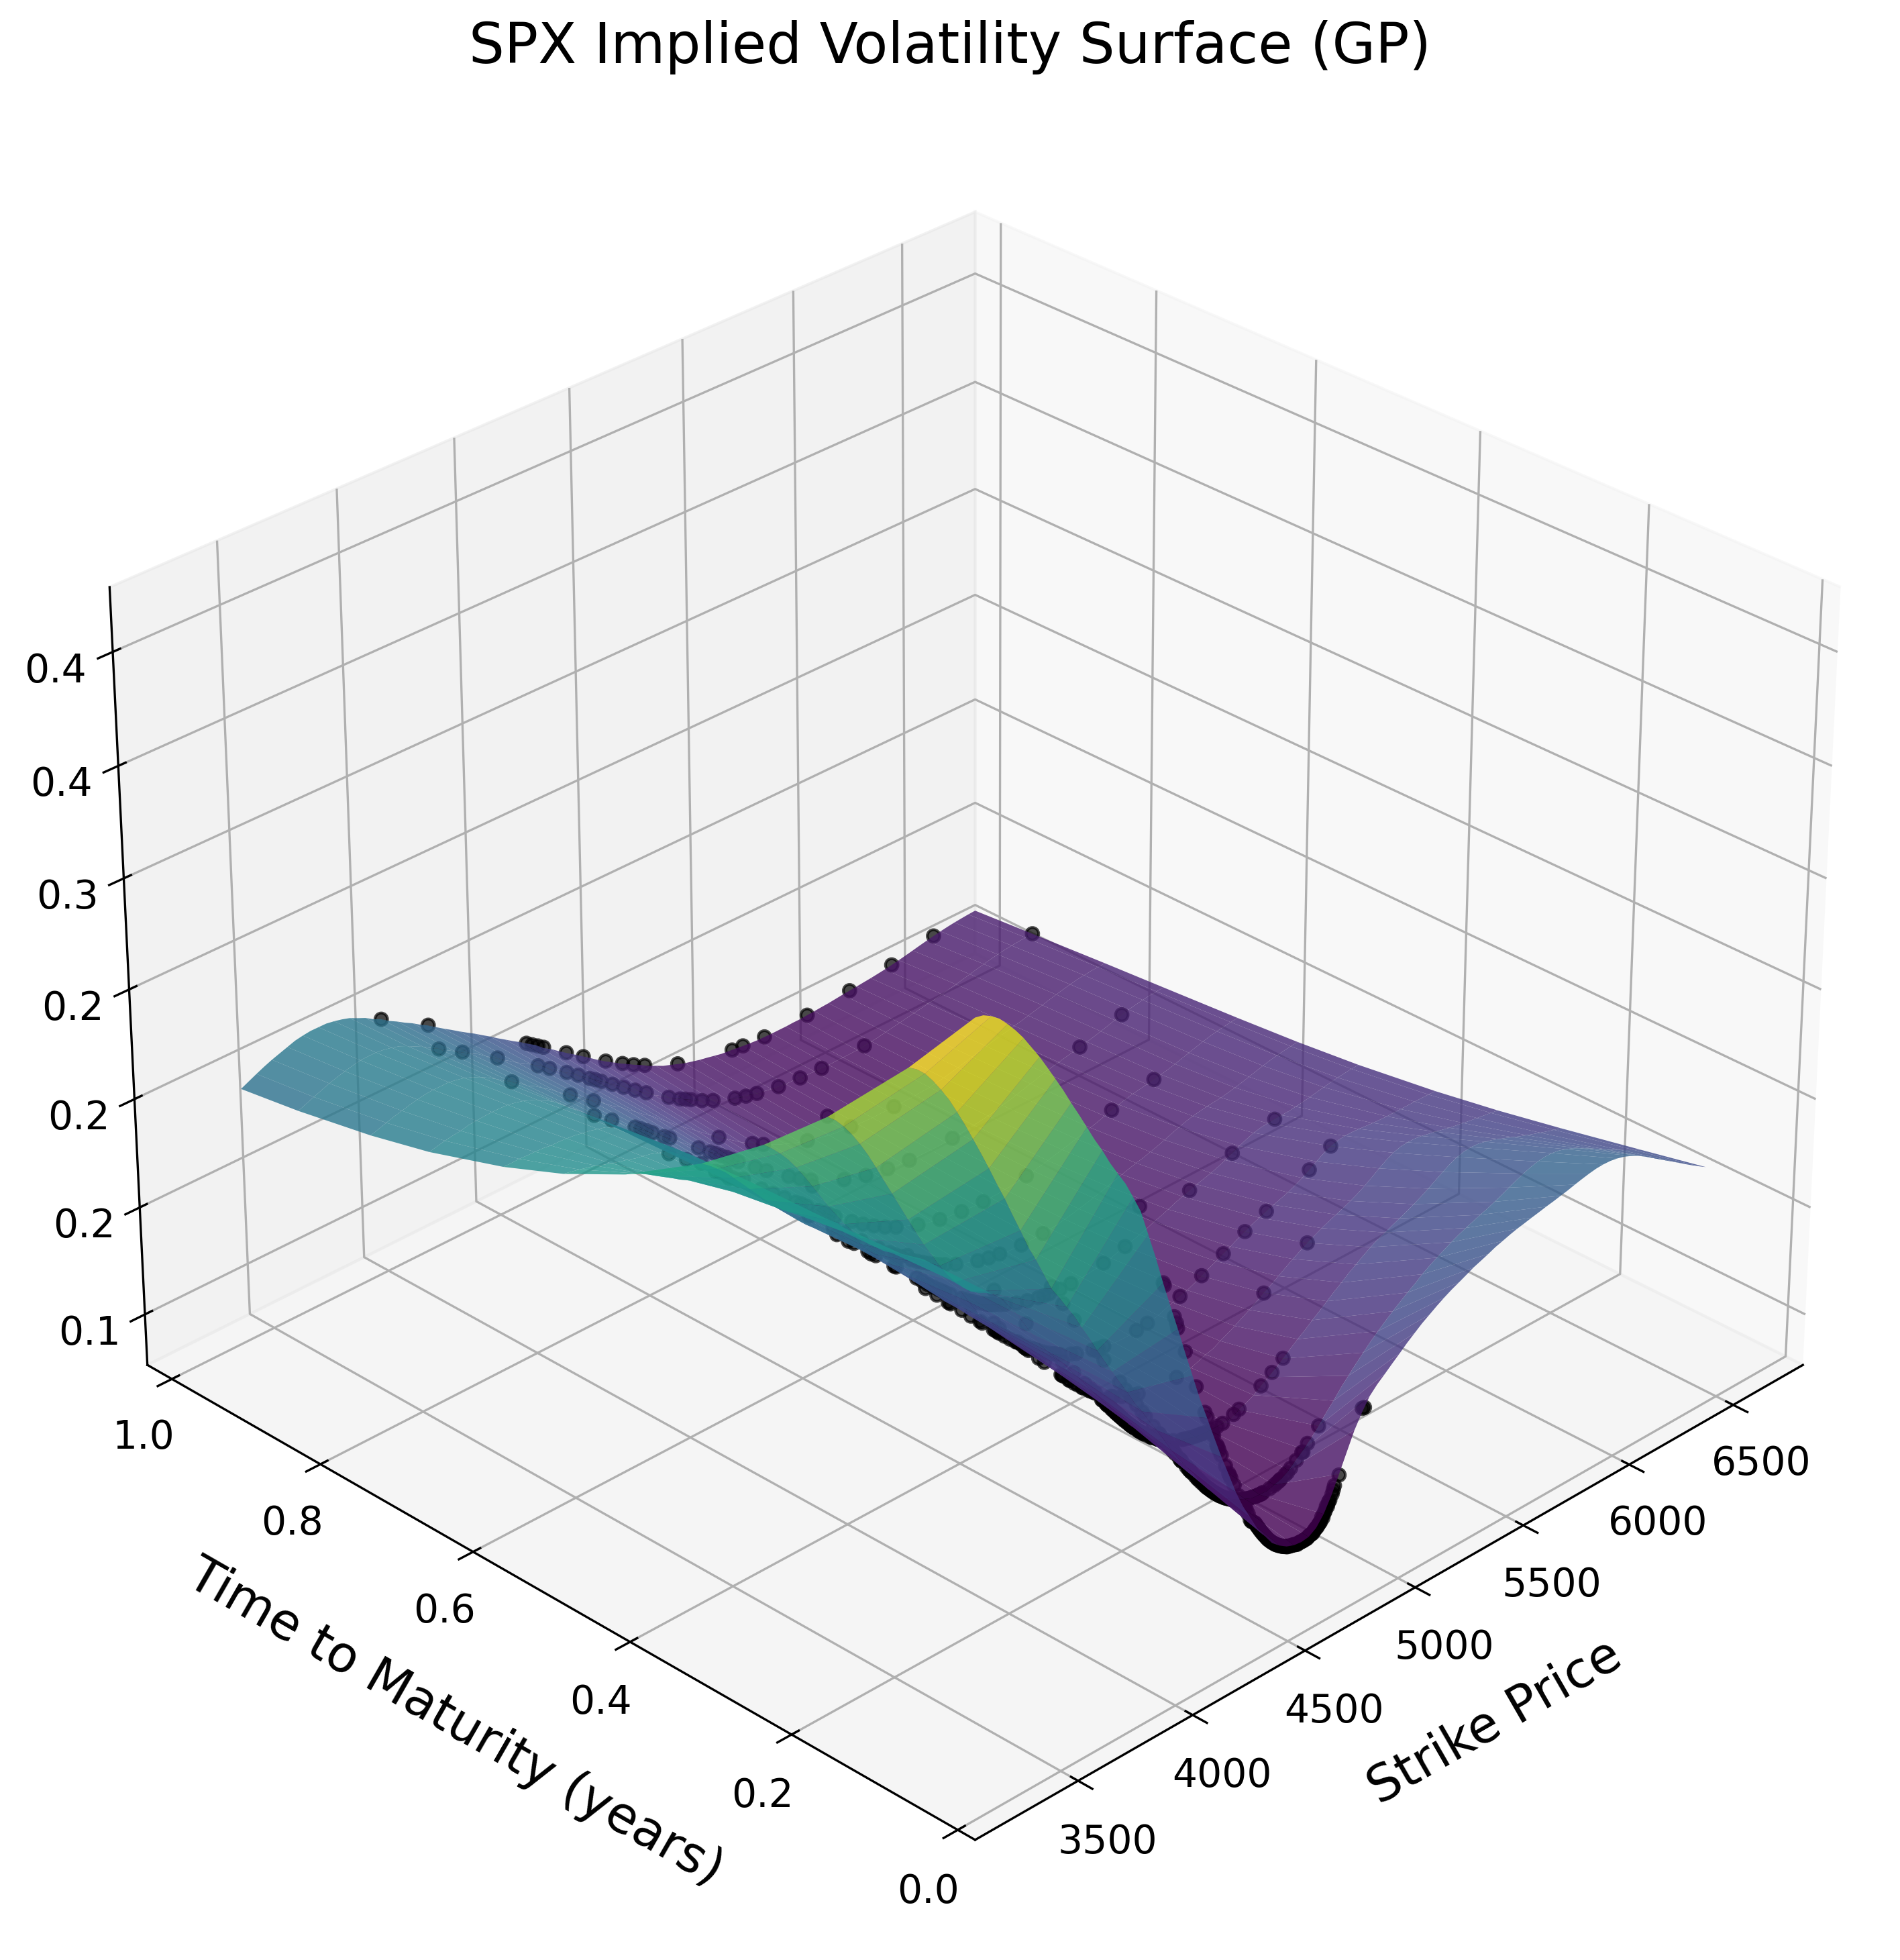
\includegraphics[width=\textwidth]{spx_iv_surface_3d_gp.png} % Ensure this file exists
        \caption{GP}
        \label{fig:spx_surface_gp_sub}
    \end{subfigure}
    \hfill % Add horizontal space
    \begin{subfigure}[b]{0.32\textwidth}
        \centering
        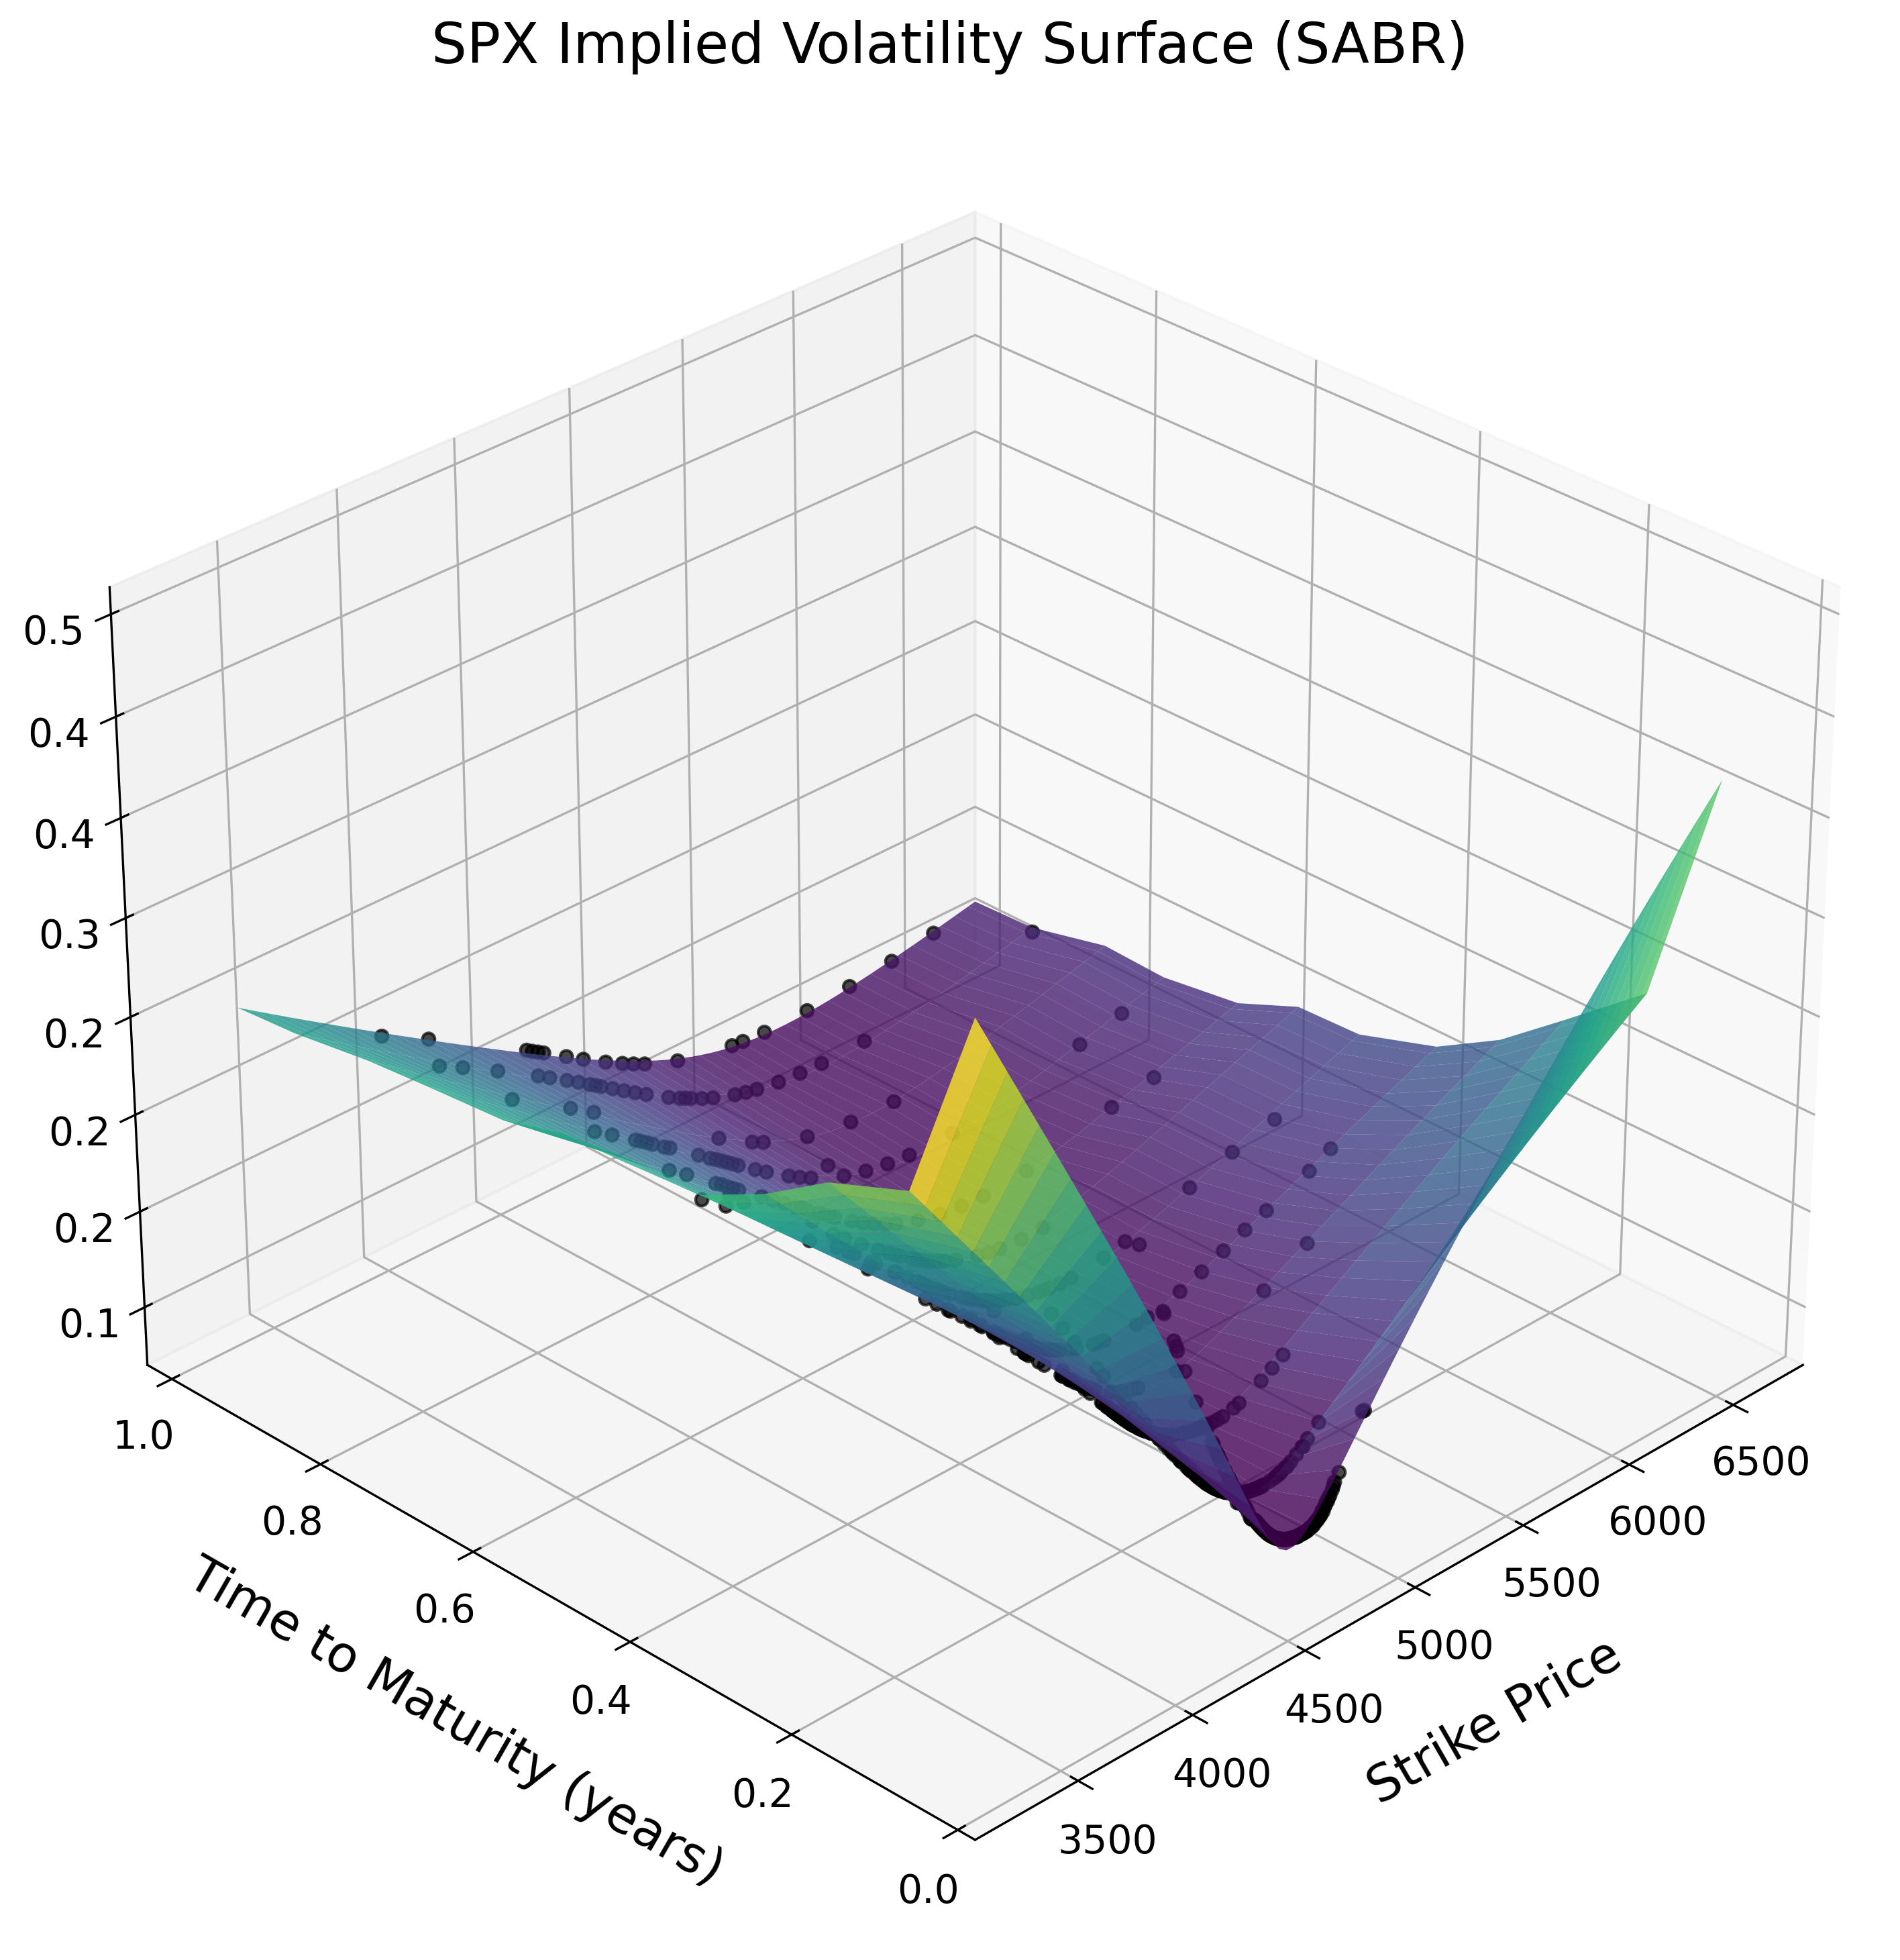
\includegraphics[width=\textwidth]{spx_iv_surface_3d_sabr.png} % Ensure this file exists
        \caption{SABR Interpolation}
        \label{fig:spx_surface_sabr_sub}
    \end{subfigure}
    \hfill % Add horizontal space
    \begin{subfigure}[b]{0.32\textwidth}
        \centering
        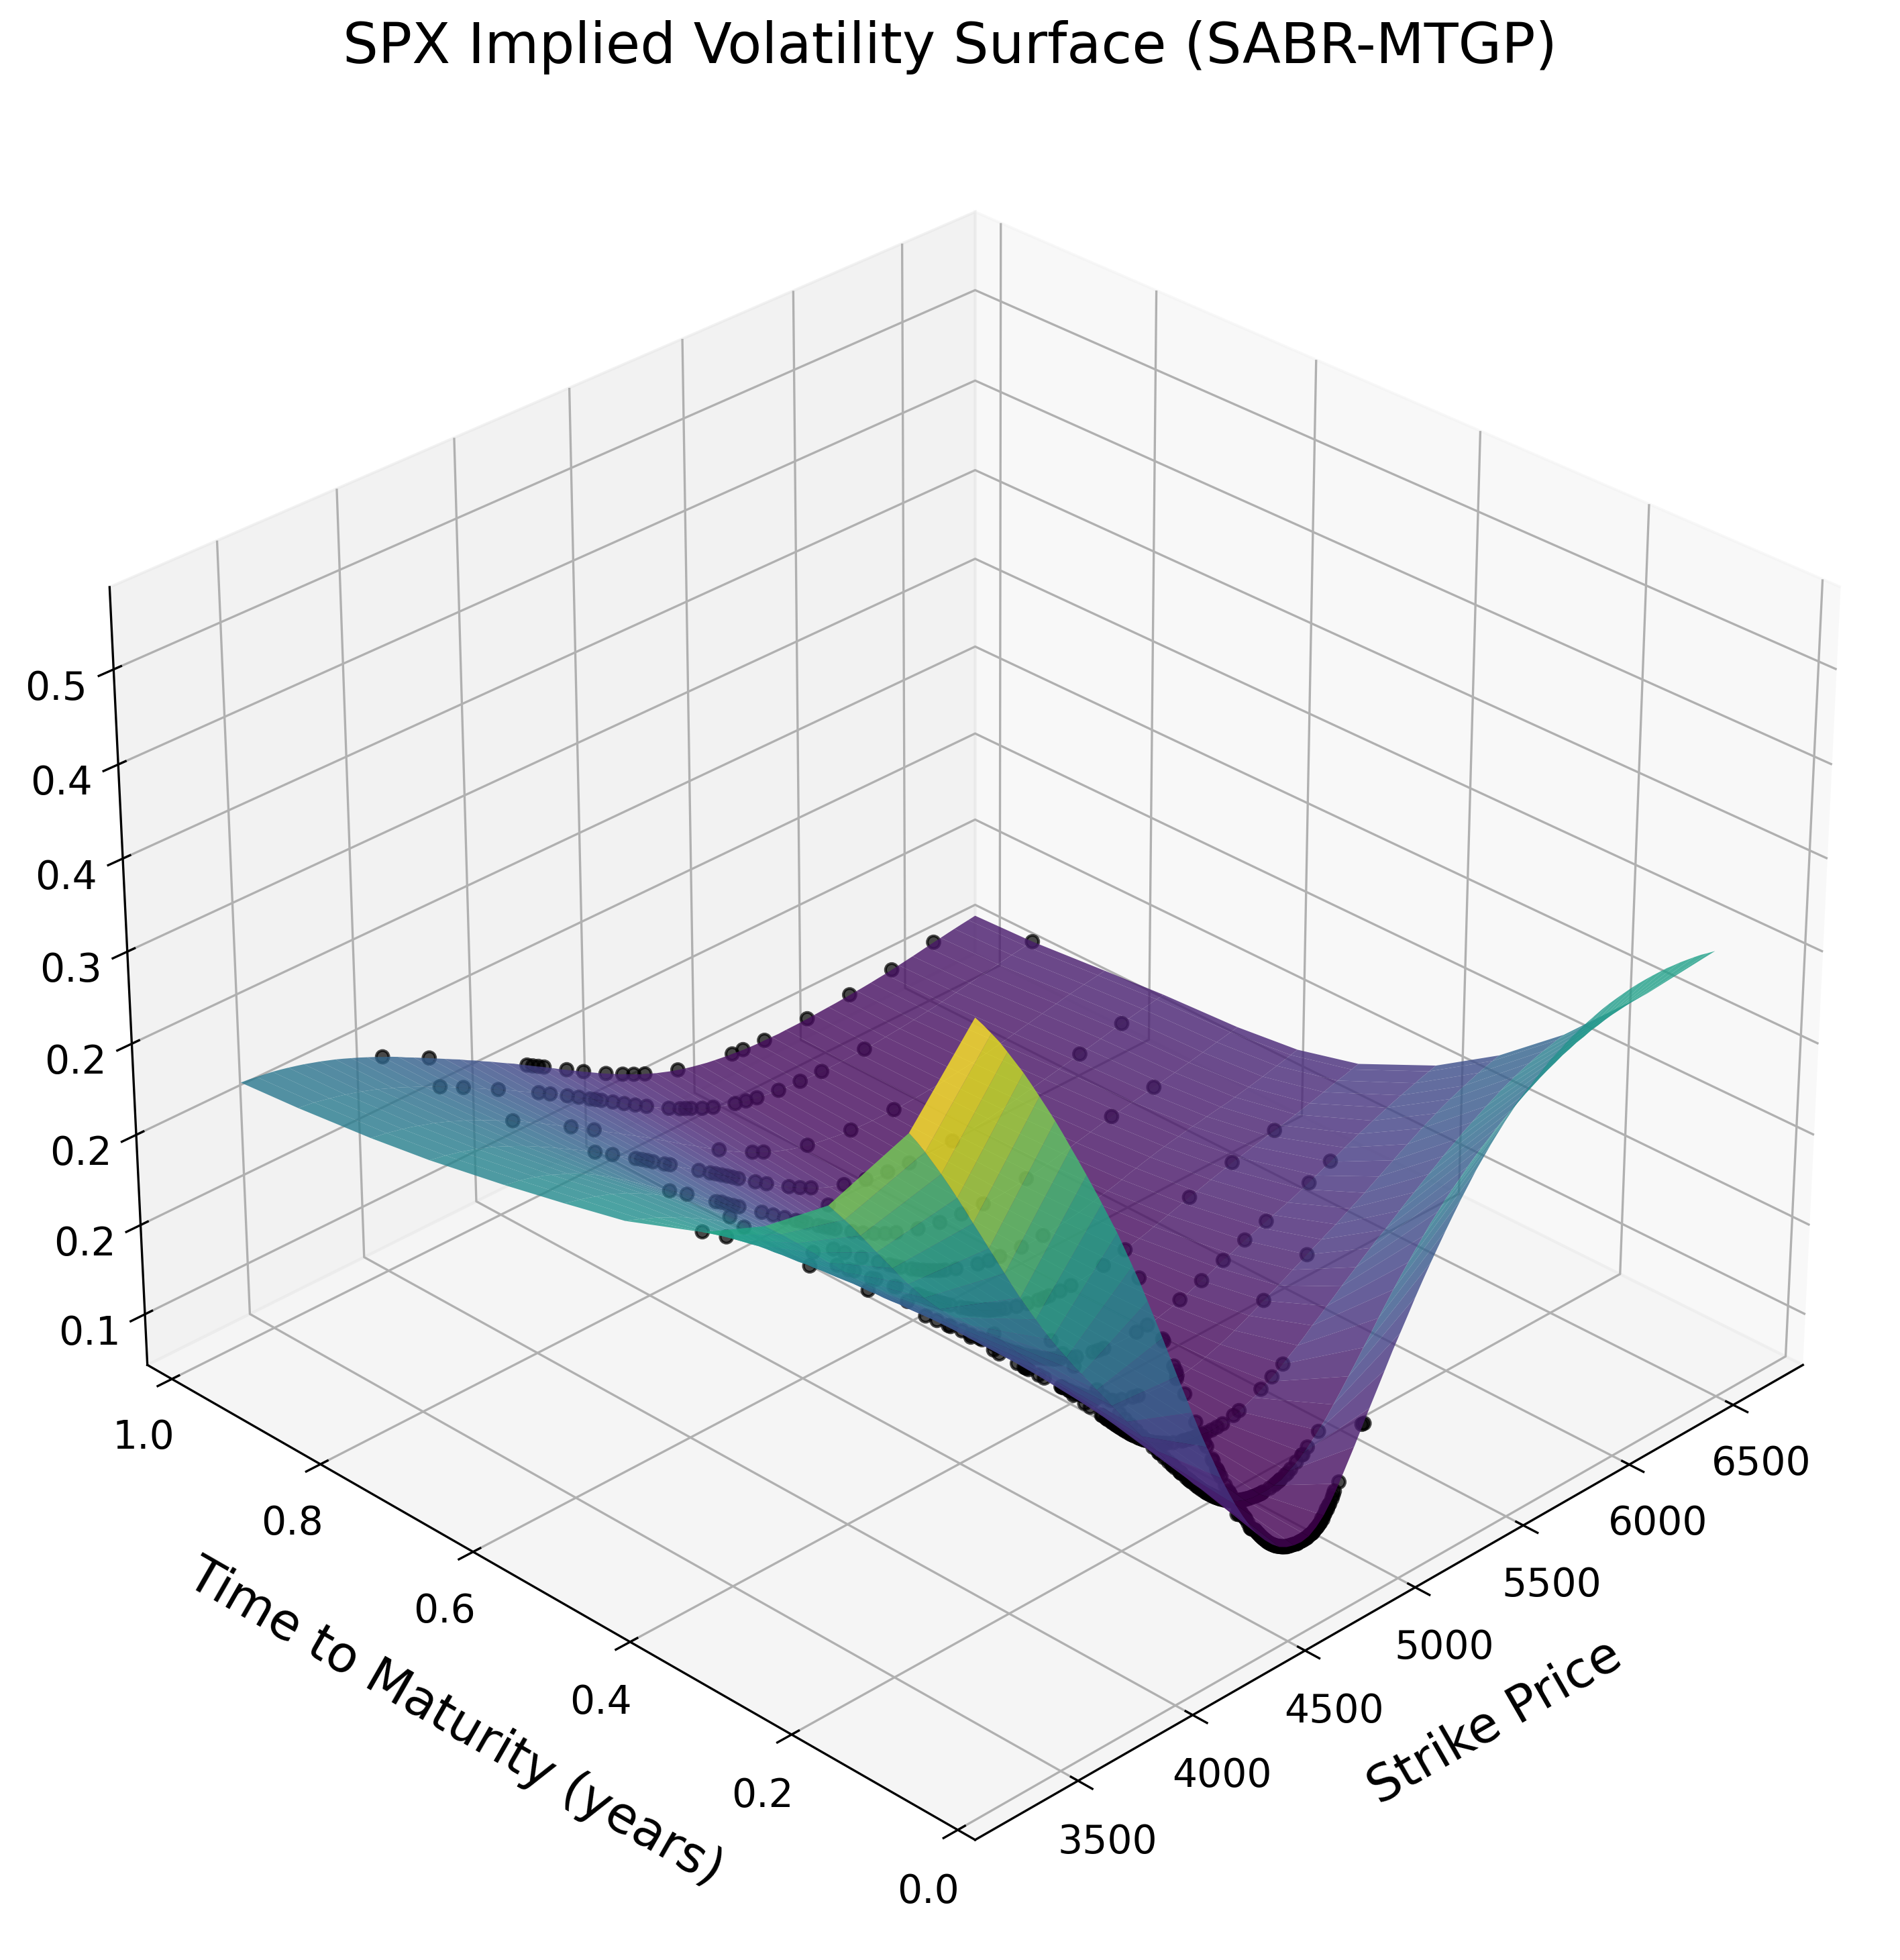
\includegraphics[width=\textwidth]{spx_iv_surface_3d_mtgp.png} % Ensure this file exists
        \caption{SABR-MTGP}
        \label{fig:spx_surface_mtgp_sub}
    \end{subfigure}
    \caption{SPX Implied Volatility Surfaces constructed using (a) GP, (b) SABR Interpolation, and (c) SABR-MTGP, based on market data from August 1, 2023. Black dots represent observed market implied volatilities.}
    \label{fig:spx_surfaces}
\end{figure}
The three plots (Figure~\ref{fig:spx_surfaces}) showed the different shapes of the implied volatility surfaces produced by the three models. The standard GP surface (Figure~\ref{fig:spx_surface_gp_sub}) matched the observed market data points very closely. However, in data-sparse regions, particularly for deep out-the-money options ($K$ is large), it showed some unusual patterns that were inconsistent with typical market behavior, such as a downward slope in volatility where an upward sloping skew is generally expected. The SABR surface (Figure~\ref{fig:spx_surface_sabr_sub}) was naturally smooth because it was based on a specific mathematical formula. But, because of this fixed structure, it might not have captured all the specific details or patterns seen in the market data. The SABR-MTGP surface (Figure~\ref{fig:spx_surface_mtgp_sub}) seemed to offer a good balance between the other two methods. It fitted the market data well, similar to the standard GP. And, it maintained a smoother and more economically consistent shape compared to the standard GP, especially when extending to areas with less data, such as longer times-to-maturity or strike prices far from the current price. This visual comparison suggested that the SABR-MTGP model successfully used the general structure of the SABR model to guide the construction of the surface, particularly where market data was sparse. This helped to create a more stable and realistic surface overall.


In summary, the application to real SPX market data showed the model's ability to integrate structural financial knowledge with sparse empirical observations. This led to well-behaved and plausible implied volatility surfaces suitable for practical applications.


\section{Conclusion}

In this paper, we proposed SABR-MTGP, an approach bridging structural and data-driven methods for IVS construction. The key idea is framing IVS construction as a multi-task learning problem where we used structural information from the SABR model to improve predictions from sparse market data.

Our approach offered several contributions. First, we show how to combine financial models with machine learning techniques. We used SABR as a complementary information source within our multi-task framework. Second, we developed a hierarchical Bayesian regularization for task embeddings that adaptively determined the level of information transfer. Third, our evaluation using Heston ground truth data showed this approach balanced structure and flexibility. It provided reliable predictions across market conditions and outperformed standard Gaussian process particularly in data-sparse regions. Improvements were notable for longer maturities and extreme strikes, where market data was limited. Finally, an application to real SPX market data further illustrated the model's ability to produce smooth, reliable IVS that respect market observations while benefiting from structural guidance.

Our work has practical implications for quantitative finance. SABR-MTGP provides a more reliable tool for IVS construction, crucial for derivative pricing, hedging, and risk management. By incorporating structural knowledge and empirical observations, it reduced model misspecification risk while maintaining adaptability to market realities. Future research could extend the multi-task framework to other structural models or multiple models simultaneously.
\bibliographystyle{elsarticle-num-names} 
\bibliography{reference}

\end{document}
